\documentclass[twoside]{book}

% Packages required by doxygen
\usepackage{fixltx2e}
\usepackage{calc}
\usepackage{doxygen}
\usepackage[export]{adjustbox} % also loads graphicx
\usepackage{graphicx}
\usepackage[utf8]{inputenc}
\usepackage{makeidx}
\usepackage{multicol}
\usepackage{multirow}
\PassOptionsToPackage{warn}{textcomp}
\usepackage{textcomp}
\usepackage[nointegrals]{wasysym}
\usepackage[table]{xcolor}

% Font selection
\usepackage[T1]{fontenc}
\usepackage[scaled=.90]{helvet}
\usepackage{courier}
\usepackage{amssymb}
\usepackage{sectsty}
\renewcommand{\familydefault}{\sfdefault}
\allsectionsfont{%
  \fontseries{bc}\selectfont%
  \color{darkgray}%
}
\renewcommand{\DoxyLabelFont}{%
  \fontseries{bc}\selectfont%
  \color{darkgray}%
}
\newcommand{\+}{\discretionary{\mbox{\scriptsize$\hookleftarrow$}}{}{}}

% Page & text layout
\usepackage{geometry}
\geometry{%
  a4paper,%
  top=2.5cm,%
  bottom=2.5cm,%
  left=2.5cm,%
  right=2.5cm%
}
\tolerance=750
\hfuzz=15pt
\hbadness=750
\setlength{\emergencystretch}{15pt}
\setlength{\parindent}{0cm}
\setlength{\parskip}{3ex plus 2ex minus 2ex}
\makeatletter
\renewcommand{\paragraph}{%
  \@startsection{paragraph}{4}{0ex}{-1.0ex}{1.0ex}{%
    \normalfont\normalsize\bfseries\SS@parafont%
  }%
}
\renewcommand{\subparagraph}{%
  \@startsection{subparagraph}{5}{0ex}{-1.0ex}{1.0ex}{%
    \normalfont\normalsize\bfseries\SS@subparafont%
  }%
}
\makeatother

% Headers & footers
\usepackage{fancyhdr}
\pagestyle{fancyplain}
\fancyhead[LE]{\fancyplain{}{\bfseries\thepage}}
\fancyhead[CE]{\fancyplain{}{}}
\fancyhead[RE]{\fancyplain{}{\bfseries\leftmark}}
\fancyhead[LO]{\fancyplain{}{\bfseries\rightmark}}
\fancyhead[CO]{\fancyplain{}{}}
\fancyhead[RO]{\fancyplain{}{\bfseries\thepage}}
\fancyfoot[LE]{\fancyplain{}{}}
\fancyfoot[CE]{\fancyplain{}{}}
\fancyfoot[RE]{\fancyplain{}{\bfseries\scriptsize Generated by Doxygen }}
\fancyfoot[LO]{\fancyplain{}{\bfseries\scriptsize Generated by Doxygen }}
\fancyfoot[CO]{\fancyplain{}{}}
\fancyfoot[RO]{\fancyplain{}{}}
\renewcommand{\footrulewidth}{0.4pt}
\renewcommand{\chaptermark}[1]{%
  \markboth{#1}{}%
}
\renewcommand{\sectionmark}[1]{%
  \markright{\thesection\ #1}%
}

% Indices & bibliography
\usepackage{natbib}
\usepackage[titles]{tocloft}
\setcounter{tocdepth}{3}
\setcounter{secnumdepth}{5}
\makeindex

% Hyperlinks (required, but should be loaded last)
\usepackage{ifpdf}
\ifpdf
  \usepackage[pdftex,pagebackref=true]{hyperref}
\else
  \usepackage[ps2pdf,pagebackref=true]{hyperref}
\fi
\hypersetup{%
  colorlinks=true,%
  linkcolor=blue,%
  citecolor=blue,%
  unicode%
}

% Custom commands
\newcommand{\clearemptydoublepage}{%
  \newpage{\pagestyle{empty}\cleardoublepage}%
}

\usepackage{caption}
\captionsetup{labelsep=space,justification=centering,font={bf},singlelinecheck=off,skip=4pt,position=top}

%===== C O N T E N T S =====

\begin{document}

% Titlepage & ToC
\hypersetup{pageanchor=false,
             bookmarksnumbered=true,
             pdfencoding=unicode
            }
\pagenumbering{roman}
\begin{titlepage}
\vspace*{7cm}
\begin{center}%
{\Large My Project }\\
\vspace*{1cm}
{\large Generated by Doxygen 1.8.11}\\
\end{center}
\end{titlepage}
\clearemptydoublepage
\tableofcontents
\clearemptydoublepage
\pagenumbering{arabic}
\hypersetup{pageanchor=true}

%--- Begin generated contents ---
\chapter{R\+E\+A\+D\+ME}
\label{md_README}
\hypertarget{md_README}{}
P\+PL Assignment by Indresh Attri(\+I\+I\+T2015121)~\newline
 To see documentation go to H\+T\+ML folder in Documentation and run annotated.\+html in browser. 
\chapter{Class Index}
\section{Class List}
Here are the classes, structs, unions and interfaces with brief descriptions\+:\begin{DoxyCompactList}
\item\contentsline{section}{\hyperlink{classBoy}{Boy} }{\pageref{classBoy}}{}
\item\contentsline{section}{\hyperlink{classcouple}{couple} }{\pageref{classcouple}}{}
\item\contentsline{section}{\hyperlink{classGift}{Gift} }{\pageref{classGift}}{}
\item\contentsline{section}{\hyperlink{classGirl}{Girl} }{\pageref{classGirl}}{}
\end{DoxyCompactList}

\chapter{File Index}
\section{File List}
Here is a list of all files with brief descriptions\+:\begin{DoxyCompactList}
\item\contentsline{section}{\hyperlink{boy_8cpp}{boy.\+cpp} }{\pageref{boy_8cpp}}{}
\item\contentsline{section}{\hyperlink{boy_8h}{boy.\+h} }{\pageref{boy_8h}}{}
\item\contentsline{section}{\hyperlink{couple_8cpp}{couple.\+cpp} }{\pageref{couple_8cpp}}{}
\item\contentsline{section}{\hyperlink{couple_8h}{couple.\+h} }{\pageref{couple_8h}}{}
\item\contentsline{section}{\hyperlink{gift_8cpp}{gift.\+cpp} }{\pageref{gift_8cpp}}{}
\item\contentsline{section}{\hyperlink{gift_8h}{gift.\+h} }{\pageref{gift_8h}}{}
\item\contentsline{section}{\hyperlink{girl_8cpp}{girl.\+cpp} }{\pageref{girl_8cpp}}{}
\item\contentsline{section}{\hyperlink{girl_8h}{girl.\+h} }{\pageref{girl_8h}}{}
\item\contentsline{section}{\hyperlink{Q1_8cpp}{Q1.\+cpp} }{\pageref{Q1_8cpp}}{}
\item\contentsline{section}{\hyperlink{Q2_8cpp}{Q2.\+cpp} }{\pageref{Q2_8cpp}}{}
\end{DoxyCompactList}

\chapter{Class Documentation}
\hypertarget{classBoy}{}\section{Boy Class Reference}
\label{classBoy}\index{Boy@{Boy}}


{\ttfamily \#include $<$boy.\+h$>$}

\subsection*{Public Member Functions}
\begin{DoxyCompactItemize}
\item 
void \hyperlink{classBoy_aa6d16a472a01b4e7da0817fe94d9a2bd}{init} (std\+::string boyname, std\+::string boytype, int boyattr, int boyintelli, int boybud)
\item 
int \hyperlink{classBoy_a72ac2c3f82b5dbd6ec97bf46dfd62681}{get\+Status} ()
\item 
void \hyperlink{classBoy_a2a8cc82d9332c07eb475198e46028d52}{change\+Status} ()
\item 
void \hyperlink{classBoy_a1ffc629e12e8a14b48c5b65133af9809}{change\+Budget} (int price)
\item 
int \hyperlink{classBoy_a05c48b12091ebcad44ba86ba88514ac5}{get\+Budget} ()
\item 
int \hyperlink{classBoy_adb7888ec543c4dcba1bcb1d7e32d7ed1}{get\+Intelli} ()
\item 
int \hyperlink{classBoy_a555fc2dfb930f29fdc384f5d7013759b}{get\+Attr} ()
\item 
std\+::string \hyperlink{classBoy_acf59fd0074a6ea3413751a95b2970303}{get\+Name} ()
\item 
std\+::string \hyperlink{classBoy_a04fcc2f16f9e3d569c64d23a73d9e258}{get\+Type} ()
\end{DoxyCompactItemize}


\subsection{Member Function Documentation}
\index{Boy@{Boy}!change\+Budget@{change\+Budget}}
\index{change\+Budget@{change\+Budget}!Boy@{Boy}}
\subsubsection[{\texorpdfstring{change\+Budget(int price)}{changeBudget(int price)}}]{\setlength{\rightskip}{0pt plus 5cm}void Boy\+::change\+Budget (
\begin{DoxyParamCaption}
\item[{int}]{price}
\end{DoxyParamCaption}
)}\hypertarget{classBoy_a1ffc629e12e8a14b48c5b65133af9809}{}\label{classBoy_a1ffc629e12e8a14b48c5b65133af9809}
\index{Boy@{Boy}!change\+Status@{change\+Status}}
\index{change\+Status@{change\+Status}!Boy@{Boy}}
\subsubsection[{\texorpdfstring{change\+Status()}{changeStatus()}}]{\setlength{\rightskip}{0pt plus 5cm}void Boy\+::change\+Status (
\begin{DoxyParamCaption}
{}
\end{DoxyParamCaption}
)}\hypertarget{classBoy_a2a8cc82d9332c07eb475198e46028d52}{}\label{classBoy_a2a8cc82d9332c07eb475198e46028d52}
\index{Boy@{Boy}!get\+Attr@{get\+Attr}}
\index{get\+Attr@{get\+Attr}!Boy@{Boy}}
\subsubsection[{\texorpdfstring{get\+Attr()}{getAttr()}}]{\setlength{\rightskip}{0pt plus 5cm}int Boy\+::get\+Attr (
\begin{DoxyParamCaption}
{}
\end{DoxyParamCaption}
)}\hypertarget{classBoy_a555fc2dfb930f29fdc384f5d7013759b}{}\label{classBoy_a555fc2dfb930f29fdc384f5d7013759b}
\index{Boy@{Boy}!get\+Budget@{get\+Budget}}
\index{get\+Budget@{get\+Budget}!Boy@{Boy}}
\subsubsection[{\texorpdfstring{get\+Budget()}{getBudget()}}]{\setlength{\rightskip}{0pt plus 5cm}int Boy\+::get\+Budget (
\begin{DoxyParamCaption}
{}
\end{DoxyParamCaption}
)}\hypertarget{classBoy_a05c48b12091ebcad44ba86ba88514ac5}{}\label{classBoy_a05c48b12091ebcad44ba86ba88514ac5}
\index{Boy@{Boy}!get\+Intelli@{get\+Intelli}}
\index{get\+Intelli@{get\+Intelli}!Boy@{Boy}}
\subsubsection[{\texorpdfstring{get\+Intelli()}{getIntelli()}}]{\setlength{\rightskip}{0pt plus 5cm}int Boy\+::get\+Intelli (
\begin{DoxyParamCaption}
{}
\end{DoxyParamCaption}
)}\hypertarget{classBoy_adb7888ec543c4dcba1bcb1d7e32d7ed1}{}\label{classBoy_adb7888ec543c4dcba1bcb1d7e32d7ed1}
\index{Boy@{Boy}!get\+Name@{get\+Name}}
\index{get\+Name@{get\+Name}!Boy@{Boy}}
\subsubsection[{\texorpdfstring{get\+Name()}{getName()}}]{\setlength{\rightskip}{0pt plus 5cm}std\+::string Boy\+::get\+Name (
\begin{DoxyParamCaption}
{}
\end{DoxyParamCaption}
)}\hypertarget{classBoy_acf59fd0074a6ea3413751a95b2970303}{}\label{classBoy_acf59fd0074a6ea3413751a95b2970303}
\index{Boy@{Boy}!get\+Status@{get\+Status}}
\index{get\+Status@{get\+Status}!Boy@{Boy}}
\subsubsection[{\texorpdfstring{get\+Status()}{getStatus()}}]{\setlength{\rightskip}{0pt plus 5cm}int Boy\+::get\+Status (
\begin{DoxyParamCaption}
{}
\end{DoxyParamCaption}
)}\hypertarget{classBoy_a72ac2c3f82b5dbd6ec97bf46dfd62681}{}\label{classBoy_a72ac2c3f82b5dbd6ec97bf46dfd62681}
\index{Boy@{Boy}!get\+Type@{get\+Type}}
\index{get\+Type@{get\+Type}!Boy@{Boy}}
\subsubsection[{\texorpdfstring{get\+Type()}{getType()}}]{\setlength{\rightskip}{0pt plus 5cm}std\+::string Boy\+::get\+Type (
\begin{DoxyParamCaption}
{}
\end{DoxyParamCaption}
)}\hypertarget{classBoy_a04fcc2f16f9e3d569c64d23a73d9e258}{}\label{classBoy_a04fcc2f16f9e3d569c64d23a73d9e258}
\index{Boy@{Boy}!init@{init}}
\index{init@{init}!Boy@{Boy}}
\subsubsection[{\texorpdfstring{init(std\+::string boyname, std\+::string boytype, int boyattr, int boyintelli, int boybud)}{init(std::string boyname, std::string boytype, int boyattr, int boyintelli, int boybud)}}]{\setlength{\rightskip}{0pt plus 5cm}void Boy\+::init (
\begin{DoxyParamCaption}
\item[{std\+::string}]{boyname, }
\item[{std\+::string}]{boytype, }
\item[{int}]{boyattr, }
\item[{int}]{boyintelli, }
\item[{int}]{boybud}
\end{DoxyParamCaption}
)}\hypertarget{classBoy_aa6d16a472a01b4e7da0817fe94d9a2bd}{}\label{classBoy_aa6d16a472a01b4e7da0817fe94d9a2bd}


The documentation for this class was generated from the following files\+:\begin{DoxyCompactItemize}
\item 
\hyperlink{boy_8h}{boy.\+h}\item 
\hyperlink{boy_8cpp}{boy.\+cpp}\end{DoxyCompactItemize}

\hypertarget{classcouple}{}\section{couple Class Reference}
\label{classcouple}\index{couple@{couple}}


{\ttfamily \#include $<$couple.\+h$>$}

\subsection*{Public Member Functions}
\begin{DoxyCompactItemize}
\item 
void \hyperlink{classcouple_aaaadc39a9f265907581925ef579c7214}{set\+Happiness} ()
\item 
void \hyperlink{classcouple_a91bc77488fe8b5d30643b9ff0a56d359}{set\+Compatibility} ()
\item 
int \hyperlink{classcouple_a43d2852ce692307280ba9ab2366c16eb}{get\+Compatibility} ()
\item 
int \hyperlink{classcouple_a31d0a1c8acff06a64ebc2e2f6d9a68b1}{get\+Happiness} ()
\item 
void \hyperlink{classcouple_a3ee36a530603865ff58470bae84da220}{init} (std\+::string boy, std\+::string type, std\+::string girl, int bud, int maint, int boyattr, int girlattr, int boyintelli, int girlintelli)
\item 
int \hyperlink{classcouple_a92496b42f9d1392013c4d7456318ad70}{get\+Budget} ()
\item 
std\+::string \hyperlink{classcouple_afe07f86e775d20508e6cd139488af366}{get\+Boyname} ()
\item 
std\+::string \hyperlink{classcouple_a7897320b780dbeaa85380c71803de9c2}{get\+Girlname} ()
\item 
void \hyperlink{classcouple_a50a890cb7ffd3a44f0201b8e0d84f744}{set\+Boy\+Happiness} (int hap)
\item 
void \hyperlink{classcouple_a526f48a752f261212d111a630f5730f4}{set\+Girl\+Happiness} (int hap)
\item 
int \hyperlink{classcouple_ada2f9b79cede186a0e9bcd6b48bec804}{get\+Girl\+Happiness} ()
\item 
void \hyperlink{classcouple_afa9889ca750dd53ffd06daf78cbee326}{change\+Curr\+Budget} (int val)
\item 
int \hyperlink{classcouple_af4b090a72111d7ba566747e4e305a6ec}{get\+Curr\+Budget} ()
\item 
int \hyperlink{classcouple_a5f31ac8019f5db29694dc36cdba958b8}{get\+Cost} ()
\item 
std\+::string \hyperlink{classcouple_a687986a266cc984fa5d2114c888f52cf}{get\+Boy\+Type} ()
\end{DoxyCompactItemize}


\subsection{Member Function Documentation}
\index{couple@{couple}!change\+Curr\+Budget@{change\+Curr\+Budget}}
\index{change\+Curr\+Budget@{change\+Curr\+Budget}!couple@{couple}}
\subsubsection[{\texorpdfstring{change\+Curr\+Budget(int val)}{changeCurrBudget(int val)}}]{\setlength{\rightskip}{0pt plus 5cm}void couple\+::change\+Curr\+Budget (
\begin{DoxyParamCaption}
\item[{int}]{val}
\end{DoxyParamCaption}
)}\hypertarget{classcouple_afa9889ca750dd53ffd06daf78cbee326}{}\label{classcouple_afa9889ca750dd53ffd06daf78cbee326}

\begin{DoxyCode}
23                                       \{
24     curBudget = curBudget - val;
25     giftPrice += val;
26 \}
\end{DoxyCode}
\index{couple@{couple}!get\+Boyname@{get\+Boyname}}
\index{get\+Boyname@{get\+Boyname}!couple@{couple}}
\subsubsection[{\texorpdfstring{get\+Boyname()}{getBoyname()}}]{\setlength{\rightskip}{0pt plus 5cm}std\+::string couple\+::get\+Boyname (
\begin{DoxyParamCaption}
{}
\end{DoxyParamCaption}
)}\hypertarget{classcouple_afe07f86e775d20508e6cd139488af366}{}\label{classcouple_afe07f86e775d20508e6cd139488af366}

\begin{DoxyCode}
40                                \{
41     \textcolor{keywordflow}{return} boyname;
42 \}
\end{DoxyCode}
\index{couple@{couple}!get\+Boy\+Type@{get\+Boy\+Type}}
\index{get\+Boy\+Type@{get\+Boy\+Type}!couple@{couple}}
\subsubsection[{\texorpdfstring{get\+Boy\+Type()}{getBoyType()}}]{\setlength{\rightskip}{0pt plus 5cm}std\+::string couple\+::get\+Boy\+Type (
\begin{DoxyParamCaption}
{}
\end{DoxyParamCaption}
)}\hypertarget{classcouple_a687986a266cc984fa5d2114c888f52cf}{}\label{classcouple_a687986a266cc984fa5d2114c888f52cf}

\begin{DoxyCode}
32                               \{
33     \textcolor{keywordflow}{return} boyType;
34 \}
\end{DoxyCode}
\index{couple@{couple}!get\+Budget@{get\+Budget}}
\index{get\+Budget@{get\+Budget}!couple@{couple}}
\subsubsection[{\texorpdfstring{get\+Budget()}{getBudget()}}]{\setlength{\rightskip}{0pt plus 5cm}int couple\+::get\+Budget (
\begin{DoxyParamCaption}
{}
\end{DoxyParamCaption}
)}\hypertarget{classcouple_a92496b42f9d1392013c4d7456318ad70}{}\label{classcouple_a92496b42f9d1392013c4d7456318ad70}

\begin{DoxyCode}
36                       \{
37     \textcolor{keywordflow}{return} boybudget;
38 \}
\end{DoxyCode}
\index{couple@{couple}!get\+Compatibility@{get\+Compatibility}}
\index{get\+Compatibility@{get\+Compatibility}!couple@{couple}}
\subsubsection[{\texorpdfstring{get\+Compatibility()}{getCompatibility()}}]{\setlength{\rightskip}{0pt plus 5cm}int couple\+::get\+Compatibility (
\begin{DoxyParamCaption}
{}
\end{DoxyParamCaption}
)}\hypertarget{classcouple_a43d2852ce692307280ba9ab2366c16eb}{}\label{classcouple_a43d2852ce692307280ba9ab2366c16eb}

\begin{DoxyCode}
72                               \{
73     \textcolor{keywordflow}{return} compatibility;
74 \}\end{DoxyCode}
\index{couple@{couple}!get\+Cost@{get\+Cost}}
\index{get\+Cost@{get\+Cost}!couple@{couple}}
\subsubsection[{\texorpdfstring{get\+Cost()}{getCost()}}]{\setlength{\rightskip}{0pt plus 5cm}int couple\+::get\+Cost (
\begin{DoxyParamCaption}
{}
\end{DoxyParamCaption}
)}\hypertarget{classcouple_a5f31ac8019f5db29694dc36cdba958b8}{}\label{classcouple_a5f31ac8019f5db29694dc36cdba958b8}

\begin{DoxyCode}
28                      \{
29     \textcolor{keywordflow}{return} giftPrice;
30 \}
\end{DoxyCode}
\index{couple@{couple}!get\+Curr\+Budget@{get\+Curr\+Budget}}
\index{get\+Curr\+Budget@{get\+Curr\+Budget}!couple@{couple}}
\subsubsection[{\texorpdfstring{get\+Curr\+Budget()}{getCurrBudget()}}]{\setlength{\rightskip}{0pt plus 5cm}int couple\+::get\+Curr\+Budget (
\begin{DoxyParamCaption}
{}
\end{DoxyParamCaption}
)}\hypertarget{classcouple_af4b090a72111d7ba566747e4e305a6ec}{}\label{classcouple_af4b090a72111d7ba566747e4e305a6ec}

\begin{DoxyCode}
19                            \{
20     \textcolor{keywordflow}{return} curBudget;
21 \}
\end{DoxyCode}
\index{couple@{couple}!get\+Girl\+Happiness@{get\+Girl\+Happiness}}
\index{get\+Girl\+Happiness@{get\+Girl\+Happiness}!couple@{couple}}
\subsubsection[{\texorpdfstring{get\+Girl\+Happiness()}{getGirlHappiness()}}]{\setlength{\rightskip}{0pt plus 5cm}int couple\+::get\+Girl\+Happiness (
\begin{DoxyParamCaption}
{}
\end{DoxyParamCaption}
)}\hypertarget{classcouple_ada2f9b79cede186a0e9bcd6b48bec804}{}\label{classcouple_ada2f9b79cede186a0e9bcd6b48bec804}

\begin{DoxyCode}
56                               \{
57     \textcolor{keywordflow}{return} girlHappiness;
58 \}
\end{DoxyCode}
\index{couple@{couple}!get\+Girlname@{get\+Girlname}}
\index{get\+Girlname@{get\+Girlname}!couple@{couple}}
\subsubsection[{\texorpdfstring{get\+Girlname()}{getGirlname()}}]{\setlength{\rightskip}{0pt plus 5cm}std\+::string couple\+::get\+Girlname (
\begin{DoxyParamCaption}
{}
\end{DoxyParamCaption}
)}\hypertarget{classcouple_a7897320b780dbeaa85380c71803de9c2}{}\label{classcouple_a7897320b780dbeaa85380c71803de9c2}

\begin{DoxyCode}
44                                \{
45     \textcolor{keywordflow}{return} girlname;
46 \}
\end{DoxyCode}
\index{couple@{couple}!get\+Happiness@{get\+Happiness}}
\index{get\+Happiness@{get\+Happiness}!couple@{couple}}
\subsubsection[{\texorpdfstring{get\+Happiness()}{getHappiness()}}]{\setlength{\rightskip}{0pt plus 5cm}int couple\+::get\+Happiness (
\begin{DoxyParamCaption}
{}
\end{DoxyParamCaption}
)}\hypertarget{classcouple_a31d0a1c8acff06a64ebc2e2f6d9a68b1}{}\label{classcouple_a31d0a1c8acff06a64ebc2e2f6d9a68b1}

\begin{DoxyCode}
60                           \{
61     \textcolor{keywordflow}{return} happiness;
62 \}
\end{DoxyCode}
\index{couple@{couple}!init@{init}}
\index{init@{init}!couple@{couple}}
\subsubsection[{\texorpdfstring{init(std\+::string boy, std\+::string type, std\+::string girl, int bud, int maint, int boyattr, int girlattr, int boyintelli, int girlintelli)}{init(std::string boy, std::string type, std::string girl, int bud, int maint, int boyattr, int girlattr, int boyintelli, int girlintelli)}}]{\setlength{\rightskip}{0pt plus 5cm}void couple\+::init (
\begin{DoxyParamCaption}
\item[{std\+::string}]{boy, }
\item[{std\+::string}]{type, }
\item[{std\+::string}]{girl, }
\item[{int}]{bud, }
\item[{int}]{maint, }
\item[{int}]{boyattr, }
\item[{int}]{girlattr, }
\item[{int}]{boyintelli, }
\item[{int}]{girlintelli}
\end{DoxyParamCaption}
)}\hypertarget{classcouple_a3ee36a530603865ff58470bae84da220}{}\label{classcouple_a3ee36a530603865ff58470bae84da220}

\begin{DoxyCode}
5                                                                                                            
                                              \{
6     boyname = boy;
7     girlname = girl;
8     boybudget = bud;
9     girlmaint = maint;
10     curBudget = bud;
11     giftPrice = 0;
12     boyattr = boyattr;
13     boyintelli = boyintelli;
14     girlattr = girlattr;
15     girlintelli = girlintelli;
16     boyType = type;
17 \}
\end{DoxyCode}
\index{couple@{couple}!set\+Boy\+Happiness@{set\+Boy\+Happiness}}
\index{set\+Boy\+Happiness@{set\+Boy\+Happiness}!couple@{couple}}
\subsubsection[{\texorpdfstring{set\+Boy\+Happiness(int hap)}{setBoyHappiness(int hap)}}]{\setlength{\rightskip}{0pt plus 5cm}void couple\+::set\+Boy\+Happiness (
\begin{DoxyParamCaption}
\item[{int}]{hap}
\end{DoxyParamCaption}
)}\hypertarget{classcouple_a50a890cb7ffd3a44f0201b8e0d84f744}{}\label{classcouple_a50a890cb7ffd3a44f0201b8e0d84f744}

\begin{DoxyCode}
48                                      \{
49     boyHappiness = hap;
50 \}
\end{DoxyCode}
\index{couple@{couple}!set\+Compatibility@{set\+Compatibility}}
\index{set\+Compatibility@{set\+Compatibility}!couple@{couple}}
\subsubsection[{\texorpdfstring{set\+Compatibility()}{setCompatibility()}}]{\setlength{\rightskip}{0pt plus 5cm}void couple\+::set\+Compatibility (
\begin{DoxyParamCaption}
{}
\end{DoxyParamCaption}
)}\hypertarget{classcouple_a91bc77488fe8b5d30643b9ff0a56d359}{}\label{classcouple_a91bc77488fe8b5d30643b9ff0a56d359}

\begin{DoxyCode}
68                                \{
69     compatibility = std::abs(boybudget - girlmaint) + std::abs(girlattr - boyattr) + std::abs(girlintelli -
       boyintelli);
70 \}
\end{DoxyCode}
\index{couple@{couple}!set\+Girl\+Happiness@{set\+Girl\+Happiness}}
\index{set\+Girl\+Happiness@{set\+Girl\+Happiness}!couple@{couple}}
\subsubsection[{\texorpdfstring{set\+Girl\+Happiness(int hap)}{setGirlHappiness(int hap)}}]{\setlength{\rightskip}{0pt plus 5cm}void couple\+::set\+Girl\+Happiness (
\begin{DoxyParamCaption}
\item[{int}]{hap}
\end{DoxyParamCaption}
)}\hypertarget{classcouple_a526f48a752f261212d111a630f5730f4}{}\label{classcouple_a526f48a752f261212d111a630f5730f4}

\begin{DoxyCode}
52                                       \{
53     girlHappiness = hap;
54 \}
\end{DoxyCode}
\index{couple@{couple}!set\+Happiness@{set\+Happiness}}
\index{set\+Happiness@{set\+Happiness}!couple@{couple}}
\subsubsection[{\texorpdfstring{set\+Happiness()}{setHappiness()}}]{\setlength{\rightskip}{0pt plus 5cm}void couple\+::set\+Happiness (
\begin{DoxyParamCaption}
{}
\end{DoxyParamCaption}
)}\hypertarget{classcouple_aaaadc39a9f265907581925ef579c7214}{}\label{classcouple_aaaadc39a9f265907581925ef579c7214}

\begin{DoxyCode}
64                            \{
65     happiness = girlHappiness + boyHappiness;
66 \}
\end{DoxyCode}


The documentation for this class was generated from the following files\+:\begin{DoxyCompactItemize}
\item 
\hyperlink{couple_8h}{couple.\+h}\item 
\hyperlink{couple_8cpp}{couple.\+cpp}\end{DoxyCompactItemize}

\hypertarget{classGift}{}\section{Gift Class Reference}
\label{classGift}\index{Gift@{Gift}}


{\ttfamily \#include $<$gift.\+h$>$}

\subsection*{Public Member Functions}
\begin{DoxyCompactItemize}
\item 
void \hyperlink{classGift_aee7c5672f4d1ee738a7dbeb6f952fe1f}{init} (int val, int pr, std\+::string ty)
\item 
int \hyperlink{classGift_aa114ca9629b5f02e4df6731d33c69373}{get\+Price} ()
\end{DoxyCompactItemize}


\subsection{Member Function Documentation}
\index{Gift@{Gift}!get\+Price@{get\+Price}}
\index{get\+Price@{get\+Price}!Gift@{Gift}}
\subsubsection[{\texorpdfstring{get\+Price()}{getPrice()}}]{\setlength{\rightskip}{0pt plus 5cm}int Gift\+::get\+Price (
\begin{DoxyParamCaption}
{}
\end{DoxyParamCaption}
)}\hypertarget{classGift_aa114ca9629b5f02e4df6731d33c69373}{}\label{classGift_aa114ca9629b5f02e4df6731d33c69373}
\index{Gift@{Gift}!init@{init}}
\index{init@{init}!Gift@{Gift}}
\subsubsection[{\texorpdfstring{init(int val, int pr, std\+::string ty)}{init(int val, int pr, std::string ty)}}]{\setlength{\rightskip}{0pt plus 5cm}void Gift\+::init (
\begin{DoxyParamCaption}
\item[{int}]{val, }
\item[{int}]{pr, }
\item[{std\+::string}]{ty}
\end{DoxyParamCaption}
)}\hypertarget{classGift_aee7c5672f4d1ee738a7dbeb6f952fe1f}{}\label{classGift_aee7c5672f4d1ee738a7dbeb6f952fe1f}


The documentation for this class was generated from the following files\+:\begin{DoxyCompactItemize}
\item 
\hyperlink{gift_8h}{gift.\+h}\item 
\hyperlink{gift_8cpp}{gift.\+cpp}\end{DoxyCompactItemize}

\hypertarget{classGirl}{}\section{Girl Class Reference}
\label{classGirl}\index{Girl@{Girl}}


{\ttfamily \#include $<$girl.\+h$>$}

\subsection*{Public Member Functions}
\begin{DoxyCompactItemize}
\item 
void \hyperlink{classGirl_aba849734c908a23bde2e5bd9c335c450}{init} (std\+::string girlname, std\+::string girltype, int girlattr, int girlintelli, int girlmaint)
\item 
int \hyperlink{classGirl_af8412c80e48e58d5e19f85f30300f8cf}{get\+Status} ()
\item 
int \hyperlink{classGirl_afe73c4c4f180aa8f5e0bc4f87455ec0b}{get\+Intelligence} ()
\item 
void \hyperlink{classGirl_ac4e040efdf40d12044bda1b647e0d2da}{change\+Status} ()
\item 
int \hyperlink{classGirl_ac23543169a5e339a3c93fbd8aeb977ca}{get\+Maint} ()
\item 
int \hyperlink{classGirl_abd8da71b97ba687e49f8d3dcd15a2cc5}{get\+Intelli} ()
\item 
int \hyperlink{classGirl_aa86bcd99f1fbcd2359a12b9a94e32486}{get\+Attr} ()
\item 
std\+::string \hyperlink{classGirl_a27a705fb94b92dfd6929d0bf4bcaf5e1}{get\+Name} ()
\item 
std\+::string \hyperlink{classGirl_a2b5bbd35287b7aa074f39702b564bc97}{get\+Type} ()
\end{DoxyCompactItemize}


\subsection{Member Function Documentation}
\index{Girl@{Girl}!change\+Status@{change\+Status}}
\index{change\+Status@{change\+Status}!Girl@{Girl}}
\subsubsection[{\texorpdfstring{change\+Status()}{changeStatus()}}]{\setlength{\rightskip}{0pt plus 5cm}void Girl\+::change\+Status (
\begin{DoxyParamCaption}
{}
\end{DoxyParamCaption}
)}\hypertarget{classGirl_ac4e040efdf40d12044bda1b647e0d2da}{}\label{classGirl_ac4e040efdf40d12044bda1b647e0d2da}
\index{Girl@{Girl}!get\+Attr@{get\+Attr}}
\index{get\+Attr@{get\+Attr}!Girl@{Girl}}
\subsubsection[{\texorpdfstring{get\+Attr()}{getAttr()}}]{\setlength{\rightskip}{0pt plus 5cm}int Girl\+::get\+Attr (
\begin{DoxyParamCaption}
{}
\end{DoxyParamCaption}
)}\hypertarget{classGirl_aa86bcd99f1fbcd2359a12b9a94e32486}{}\label{classGirl_aa86bcd99f1fbcd2359a12b9a94e32486}
\index{Girl@{Girl}!get\+Intelli@{get\+Intelli}}
\index{get\+Intelli@{get\+Intelli}!Girl@{Girl}}
\subsubsection[{\texorpdfstring{get\+Intelli()}{getIntelli()}}]{\setlength{\rightskip}{0pt plus 5cm}int Girl\+::get\+Intelli (
\begin{DoxyParamCaption}
{}
\end{DoxyParamCaption}
)}\hypertarget{classGirl_abd8da71b97ba687e49f8d3dcd15a2cc5}{}\label{classGirl_abd8da71b97ba687e49f8d3dcd15a2cc5}
\index{Girl@{Girl}!get\+Intelligence@{get\+Intelligence}}
\index{get\+Intelligence@{get\+Intelligence}!Girl@{Girl}}
\subsubsection[{\texorpdfstring{get\+Intelligence()}{getIntelligence()}}]{\setlength{\rightskip}{0pt plus 5cm}int Girl\+::get\+Intelligence (
\begin{DoxyParamCaption}
{}
\end{DoxyParamCaption}
)}\hypertarget{classGirl_afe73c4c4f180aa8f5e0bc4f87455ec0b}{}\label{classGirl_afe73c4c4f180aa8f5e0bc4f87455ec0b}
\index{Girl@{Girl}!get\+Maint@{get\+Maint}}
\index{get\+Maint@{get\+Maint}!Girl@{Girl}}
\subsubsection[{\texorpdfstring{get\+Maint()}{getMaint()}}]{\setlength{\rightskip}{0pt plus 5cm}int Girl\+::get\+Maint (
\begin{DoxyParamCaption}
{}
\end{DoxyParamCaption}
)}\hypertarget{classGirl_ac23543169a5e339a3c93fbd8aeb977ca}{}\label{classGirl_ac23543169a5e339a3c93fbd8aeb977ca}
\index{Girl@{Girl}!get\+Name@{get\+Name}}
\index{get\+Name@{get\+Name}!Girl@{Girl}}
\subsubsection[{\texorpdfstring{get\+Name()}{getName()}}]{\setlength{\rightskip}{0pt plus 5cm}std\+::string Girl\+::get\+Name (
\begin{DoxyParamCaption}
{}
\end{DoxyParamCaption}
)}\hypertarget{classGirl_a27a705fb94b92dfd6929d0bf4bcaf5e1}{}\label{classGirl_a27a705fb94b92dfd6929d0bf4bcaf5e1}
\index{Girl@{Girl}!get\+Status@{get\+Status}}
\index{get\+Status@{get\+Status}!Girl@{Girl}}
\subsubsection[{\texorpdfstring{get\+Status()}{getStatus()}}]{\setlength{\rightskip}{0pt plus 5cm}int Girl\+::get\+Status (
\begin{DoxyParamCaption}
{}
\end{DoxyParamCaption}
)}\hypertarget{classGirl_af8412c80e48e58d5e19f85f30300f8cf}{}\label{classGirl_af8412c80e48e58d5e19f85f30300f8cf}
\index{Girl@{Girl}!get\+Type@{get\+Type}}
\index{get\+Type@{get\+Type}!Girl@{Girl}}
\subsubsection[{\texorpdfstring{get\+Type()}{getType()}}]{\setlength{\rightskip}{0pt plus 5cm}std\+::string Girl\+::get\+Type (
\begin{DoxyParamCaption}
{}
\end{DoxyParamCaption}
)}\hypertarget{classGirl_a2b5bbd35287b7aa074f39702b564bc97}{}\label{classGirl_a2b5bbd35287b7aa074f39702b564bc97}
\index{Girl@{Girl}!init@{init}}
\index{init@{init}!Girl@{Girl}}
\subsubsection[{\texorpdfstring{init(std\+::string girlname, std\+::string girltype, int girlattr, int girlintelli, int girlmaint)}{init(std::string girlname, std::string girltype, int girlattr, int girlintelli, int girlmaint)}}]{\setlength{\rightskip}{0pt plus 5cm}void Girl\+::init (
\begin{DoxyParamCaption}
\item[{std\+::string}]{girlname, }
\item[{std\+::string}]{girltype, }
\item[{int}]{girlattr, }
\item[{int}]{girlintelli, }
\item[{int}]{girlmaint}
\end{DoxyParamCaption}
)}\hypertarget{classGirl_aba849734c908a23bde2e5bd9c335c450}{}\label{classGirl_aba849734c908a23bde2e5bd9c335c450}


The documentation for this class was generated from the following files\+:\begin{DoxyCompactItemize}
\item 
\hyperlink{girl_8h}{girl.\+h}\item 
\hyperlink{girl_8cpp}{girl.\+cpp}\end{DoxyCompactItemize}

\hypertarget{classLibrary}{}\section{Library Class Reference}
\label{classLibrary}\index{Library@{Library}}


{\ttfamily \#include $<$lib7.\+h$>$}



Collaboration diagram for Library\+:
\nopagebreak
\begin{figure}[H]
\begin{center}
\leavevmode
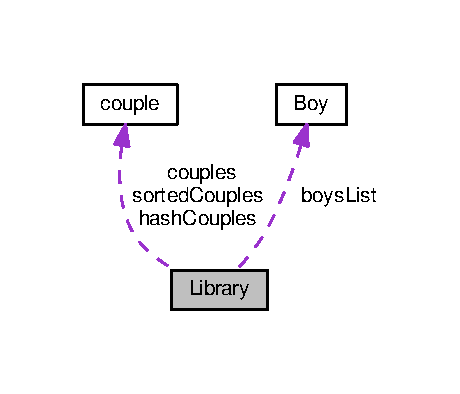
\includegraphics[width=221pt]{classLibrary__coll__graph}
\end{center}
\end{figure}
\subsection*{Public Member Functions}
\begin{DoxyCompactItemize}
\item 
void \hyperlink{classLibrary_af9853cceb7af37b77091c3330b532b2f}{search\+Arr} ()
\item 
void \hyperlink{classLibrary_a835ea2c0b31c569aac4a406843c55254}{search\+Sorted\+Arr} ()
\item 
void \hyperlink{classLibrary_ad14b4301aa6279c13408ff948ca4fd6a}{search\+Hash} ()
\end{DoxyCompactItemize}
\subsection*{Public Attributes}
\begin{DoxyCompactItemize}
\item 
\hyperlink{classcouple}{couple} $\ast$ \hyperlink{classLibrary_a6c32f4296982c3281d61d12b1add0ede}{couples}
\item 
\hyperlink{classcouple}{couple} $\ast$ \hyperlink{classLibrary_a30e860e047d63ab63b40ac42e9660f25}{sorted\+Couples}
\item 
\hyperlink{classcouple}{couple} \hyperlink{classLibrary_ac6f3af3c59edb37adb8d0becda498b42}{hash\+Couples} \mbox{[}6\mbox{]}
\item 
\hyperlink{classBoy}{Boy} \hyperlink{classLibrary_a0da9d216b9e07af39f5f0f3241a0a45c}{boys\+List} \mbox{[}9\mbox{]}
\item 
ofstream \hyperlink{classLibrary_ad8fbb4e17a98e57b3cffe8257710045d}{log\+File}
\end{DoxyCompactItemize}


\subsection{Member Function Documentation}
\index{Library@{Library}!search\+Arr@{search\+Arr}}
\index{search\+Arr@{search\+Arr}!Library@{Library}}
\subsubsection[{\texorpdfstring{search\+Arr()}{searchArr()}}]{\setlength{\rightskip}{0pt plus 5cm}void Library\+::search\+Arr (
\begin{DoxyParamCaption}
{}
\end{DoxyParamCaption}
)}\hypertarget{classLibrary_af9853cceb7af37b77091c3330b532b2f}{}\label{classLibrary_af9853cceb7af37b77091c3330b532b2f}

\begin{DoxyCode}
4 \{   
5 
6     fstream \hyperlink{classLibrary_ad8fbb4e17a98e57b3cffe8257710045d}{logFile}(\textcolor{stringliteral}{"logFile7.dat"}, std::fstream::in | std::fstream::out | std::fstream::app);
7     \hyperlink{classLibrary_ad8fbb4e17a98e57b3cffe8257710045d}{logFile}<<\textcolor{stringliteral}{"\(\backslash\)n----------You selected Linear search------------\(\backslash\)n\(\backslash\)n"};
8     \textcolor{keywordflow}{for}(\textcolor{keywordtype}{int} j = 0; j < \hyperlink{lib7_8h_a20a0f494ca2c397f664e1911db5e084b}{S}; j++) \{
9         \textcolor{keywordtype}{int} flag = 0;
10         \textcolor{keywordtype}{int} ind;
11         \textcolor{keywordflow}{for}(\textcolor{keywordtype}{int} i = 0; i < \hyperlink{lib7_8h_a5464533d23b59ba11030432e73528730}{C}; i++) \{
12 
13             \textcolor{keywordflow}{if}(\hyperlink{classLibrary_a6c32f4296982c3281d61d12b1add0ede}{couples}[i].getBoyname()[0] == \hyperlink{classLibrary_a0da9d216b9e07af39f5f0f3241a0a45c}{boysList}[j].getName()[0])\{
14 
15                 flag == 1;
16                 ind = i;        
17                 \hyperlink{classLibrary_ad8fbb4e17a98e57b3cffe8257710045d}{logFile}<<\textcolor{stringliteral}{"Boy b"}<<\hyperlink{classLibrary_a0da9d216b9e07af39f5f0f3241a0a45c}{boysList}[j].\hyperlink{classBoy_acf59fd0074a6ea3413751a95b2970303}{getName}()<<\textcolor{stringliteral}{" is commited with Girl g"}<<
      \hyperlink{classLibrary_a6c32f4296982c3281d61d12b1add0ede}{couples}[ind].\hyperlink{classcouple_a7897320b780dbeaa85380c71803de9c2}{getGirlname}()<<endl; 
18             \} 
19         \}
20     \}
21 
22 \}
\end{DoxyCode}
\index{Library@{Library}!search\+Hash@{search\+Hash}}
\index{search\+Hash@{search\+Hash}!Library@{Library}}
\subsubsection[{\texorpdfstring{search\+Hash()}{searchHash()}}]{\setlength{\rightskip}{0pt plus 5cm}void Library\+::search\+Hash (
\begin{DoxyParamCaption}
{}
\end{DoxyParamCaption}
)}\hypertarget{classLibrary_ad14b4301aa6279c13408ff948ca4fd6a}{}\label{classLibrary_ad14b4301aa6279c13408ff948ca4fd6a}

\begin{DoxyCode}
42 \{
43     fstream \hyperlink{classLibrary_ad8fbb4e17a98e57b3cffe8257710045d}{logFile}(\textcolor{stringliteral}{"logFile7.dat"}, std::fstream::in | std::fstream::out | std::fstream::app);
44     \hyperlink{classLibrary_ad8fbb4e17a98e57b3cffe8257710045d}{logFile}<<\textcolor{stringliteral}{"\(\backslash\)n-----------You selected Hash algorith-----------\(\backslash\)n\(\backslash\)n"};
45     \textcolor{keywordflow}{for}(\textcolor{keywordtype}{int} j = 0; j < \hyperlink{lib7_8h_a20a0f494ca2c397f664e1911db5e084b}{S}; j++) \{
46         \textcolor{keywordtype}{int} flag = 0;
47         \textcolor{keywordtype}{int} ind;
48         \textcolor{keywordflow}{for}(\textcolor{keywordtype}{int} i = 0; i < \hyperlink{lib7_8h_a5464533d23b59ba11030432e73528730}{C}; i++) \{
49 
50             \textcolor{keywordflow}{if}(\hyperlink{classLibrary_ac6f3af3c59edb37adb8d0becda498b42}{hashCouples}[i].getBoyname()[0] == \hyperlink{classLibrary_a0da9d216b9e07af39f5f0f3241a0a45c}{boysList}[j].getName()[0])\{
51 
52                 flag == 1;
53                 ind = i;        
54                 \hyperlink{classLibrary_ad8fbb4e17a98e57b3cffe8257710045d}{logFile}<<\textcolor{stringliteral}{"Boy b"}<<\hyperlink{classLibrary_a0da9d216b9e07af39f5f0f3241a0a45c}{boysList}[j].\hyperlink{classBoy_acf59fd0074a6ea3413751a95b2970303}{getName}()<<\textcolor{stringliteral}{" is commited with Girl g"}<<
      \hyperlink{classLibrary_ac6f3af3c59edb37adb8d0becda498b42}{hashCouples}[ind].\hyperlink{classcouple_a7897320b780dbeaa85380c71803de9c2}{getGirlname}()<<endl; 
55             \} 
56         \}
57     \}
58 \}
\end{DoxyCode}
\index{Library@{Library}!search\+Sorted\+Arr@{search\+Sorted\+Arr}}
\index{search\+Sorted\+Arr@{search\+Sorted\+Arr}!Library@{Library}}
\subsubsection[{\texorpdfstring{search\+Sorted\+Arr()}{searchSortedArr()}}]{\setlength{\rightskip}{0pt plus 5cm}void Library\+::search\+Sorted\+Arr (
\begin{DoxyParamCaption}
{}
\end{DoxyParamCaption}
)}\hypertarget{classLibrary_a835ea2c0b31c569aac4a406843c55254}{}\label{classLibrary_a835ea2c0b31c569aac4a406843c55254}

\begin{DoxyCode}
24 \{
25     fstream \hyperlink{classLibrary_ad8fbb4e17a98e57b3cffe8257710045d}{logFile}(\textcolor{stringliteral}{"logFile7.dat"}, std::fstream::in | std::fstream::out | std::fstream::app);
26     \hyperlink{classLibrary_ad8fbb4e17a98e57b3cffe8257710045d}{logFile}<<\textcolor{stringliteral}{"\(\backslash\)n--------You selected Binary Search in sorted Array---------\(\backslash\)n\(\backslash\)n"};
27     \textcolor{keywordflow}{for}(\textcolor{keywordtype}{int} j = 0; j < \hyperlink{lib7_8h_a20a0f494ca2c397f664e1911db5e084b}{S}; j++) \{
28         \textcolor{keywordtype}{int} flag = 0;
29         \textcolor{keywordtype}{int} ind;
30         \textcolor{keywordflow}{for}(\textcolor{keywordtype}{int} i = 0; i < \hyperlink{lib7_8h_a5464533d23b59ba11030432e73528730}{C}; i++) \{
31 
32             \textcolor{keywordflow}{if}(\hyperlink{classLibrary_a30e860e047d63ab63b40ac42e9660f25}{sortedCouples}[i].getBoyname()[0] == \hyperlink{classLibrary_a0da9d216b9e07af39f5f0f3241a0a45c}{boysList}[j].getName()[0])\{
33 
34                 flag == 1;
35                 ind = i;        
36                 \hyperlink{classLibrary_ad8fbb4e17a98e57b3cffe8257710045d}{logFile}<<\textcolor{stringliteral}{"Boy b"}<<\hyperlink{classLibrary_a0da9d216b9e07af39f5f0f3241a0a45c}{boysList}[j].\hyperlink{classBoy_acf59fd0074a6ea3413751a95b2970303}{getName}()<<\textcolor{stringliteral}{" is commited with Girl g"}<<
      \hyperlink{classLibrary_a30e860e047d63ab63b40ac42e9660f25}{sortedCouples}[ind].\hyperlink{classcouple_a7897320b780dbeaa85380c71803de9c2}{getGirlname}()<<endl; 
37             \} 
38         \}
39     \}
40 \}
\end{DoxyCode}


\subsection{Member Data Documentation}
\index{Library@{Library}!boys\+List@{boys\+List}}
\index{boys\+List@{boys\+List}!Library@{Library}}
\subsubsection[{\texorpdfstring{boys\+List}{boysList}}]{\setlength{\rightskip}{0pt plus 5cm}{\bf Boy} Library\+::boys\+List\mbox{[}9\mbox{]}}\hypertarget{classLibrary_a0da9d216b9e07af39f5f0f3241a0a45c}{}\label{classLibrary_a0da9d216b9e07af39f5f0f3241a0a45c}
\index{Library@{Library}!couples@{couples}}
\index{couples@{couples}!Library@{Library}}
\subsubsection[{\texorpdfstring{couples}{couples}}]{\setlength{\rightskip}{0pt plus 5cm}{\bf couple}$\ast$ Library\+::couples}\hypertarget{classLibrary_a6c32f4296982c3281d61d12b1add0ede}{}\label{classLibrary_a6c32f4296982c3281d61d12b1add0ede}
\index{Library@{Library}!hash\+Couples@{hash\+Couples}}
\index{hash\+Couples@{hash\+Couples}!Library@{Library}}
\subsubsection[{\texorpdfstring{hash\+Couples}{hashCouples}}]{\setlength{\rightskip}{0pt plus 5cm}{\bf couple} Library\+::hash\+Couples\mbox{[}6\mbox{]}}\hypertarget{classLibrary_ac6f3af3c59edb37adb8d0becda498b42}{}\label{classLibrary_ac6f3af3c59edb37adb8d0becda498b42}
\index{Library@{Library}!log\+File@{log\+File}}
\index{log\+File@{log\+File}!Library@{Library}}
\subsubsection[{\texorpdfstring{log\+File}{logFile}}]{\setlength{\rightskip}{0pt plus 5cm}ofstream Library\+::log\+File}\hypertarget{classLibrary_ad8fbb4e17a98e57b3cffe8257710045d}{}\label{classLibrary_ad8fbb4e17a98e57b3cffe8257710045d}
\index{Library@{Library}!sorted\+Couples@{sorted\+Couples}}
\index{sorted\+Couples@{sorted\+Couples}!Library@{Library}}
\subsubsection[{\texorpdfstring{sorted\+Couples}{sortedCouples}}]{\setlength{\rightskip}{0pt plus 5cm}{\bf couple}$\ast$ Library\+::sorted\+Couples}\hypertarget{classLibrary_a30e860e047d63ab63b40ac42e9660f25}{}\label{classLibrary_a30e860e047d63ab63b40ac42e9660f25}


The documentation for this class was generated from the following files\+:\begin{DoxyCompactItemize}
\item 
\hyperlink{lib7_8h}{lib7.\+h}\item 
\hyperlink{lib7_8cpp}{lib7.\+cpp}\end{DoxyCompactItemize}

\chapter{File Documentation}
\hypertarget{boy_8cpp}{}\section{boy.\+cpp File Reference}
\label{boy_8cpp}\index{boy.\+cpp@{boy.\+cpp}}
{\ttfamily \#include \char`\"{}boy.\+h\char`\"{}}\\*
{\ttfamily \#include $<$string$>$}\\*
Include dependency graph for boy.\+cpp\+:
\nopagebreak
\begin{figure}[H]
\begin{center}
\leavevmode
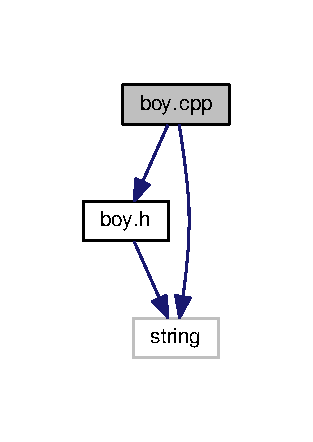
\includegraphics[width=150pt]{boy_8cpp__incl}
\end{center}
\end{figure}

\hypertarget{boy_8h}{}\section{boy.\+h File Reference}
\label{boy_8h}\index{boy.\+h@{boy.\+h}}
{\ttfamily \#include $<$string$>$}\\*
Include dependency graph for boy.\+h\+:
\nopagebreak
\begin{figure}[H]
\begin{center}
\leavevmode
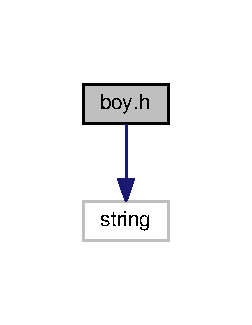
\includegraphics[width=121pt]{boy_8h__incl}
\end{center}
\end{figure}
This graph shows which files directly or indirectly include this file\+:
\nopagebreak
\begin{figure}[H]
\begin{center}
\leavevmode
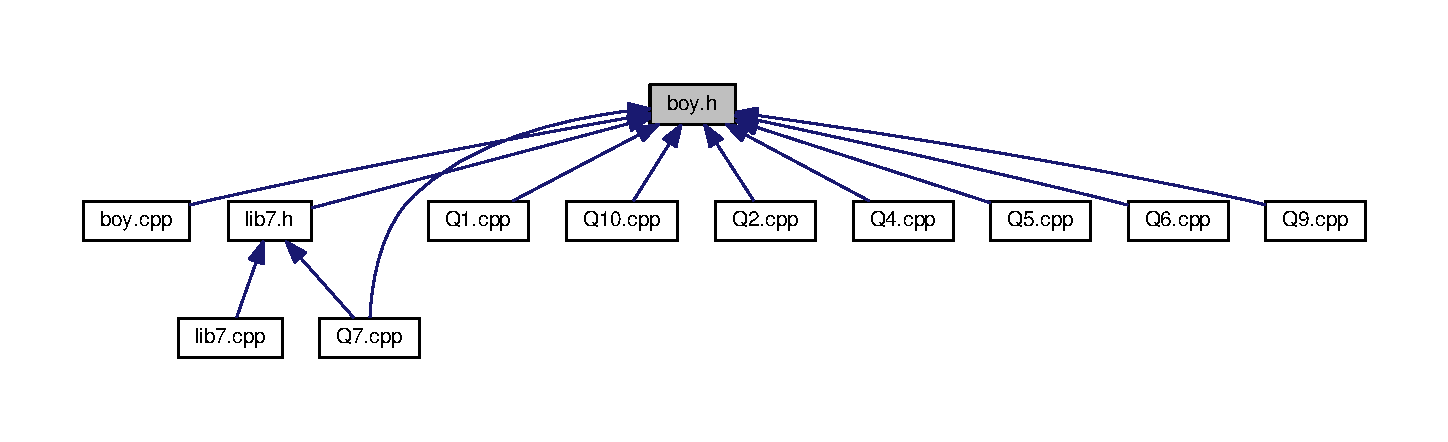
\includegraphics[width=263pt]{boy_8h__dep__incl}
\end{center}
\end{figure}
\subsection*{Classes}
\begin{DoxyCompactItemize}
\item 
class \hyperlink{classBoy}{Boy}
\end{DoxyCompactItemize}

\hypertarget{boyrec_8txt}{}\section{boyrec.\+txt File Reference}
\label{boyrec_8txt}\index{boyrec.\+txt@{boyrec.\+txt}}

\hypertarget{breakup_8txt}{}\section{breakup.\+txt File Reference}
\label{breakup_8txt}\index{breakup.\+txt@{breakup.\+txt}}

\hypertarget{couple_8cpp}{}\section{couple.\+cpp File Reference}
\label{couple_8cpp}\index{couple.\+cpp@{couple.\+cpp}}
{\ttfamily \#include \char`\"{}couple.\+h\char`\"{}}\\*
{\ttfamily \#include $<$string$>$}\\*
{\ttfamily \#include $<$cmath$>$}\\*
Include dependency graph for couple.\+cpp\+:
\nopagebreak
\begin{figure}[H]
\begin{center}
\leavevmode
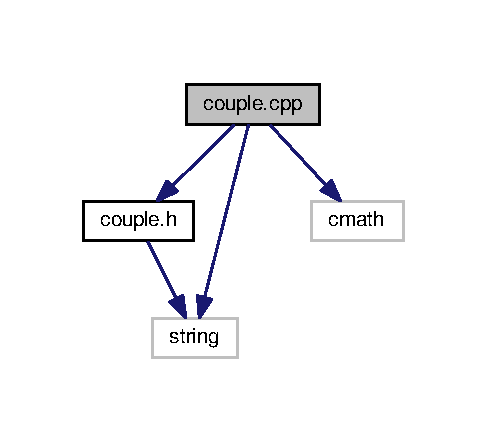
\includegraphics[width=233pt]{couple_8cpp__incl}
\end{center}
\end{figure}

\hypertarget{couple_8h}{}\section{couple.\+h File Reference}
\label{couple_8h}\index{couple.\+h@{couple.\+h}}
{\ttfamily \#include $<$string$>$}\\*
Include dependency graph for couple.\+h\+:
\nopagebreak
\begin{figure}[H]
\begin{center}
\leavevmode
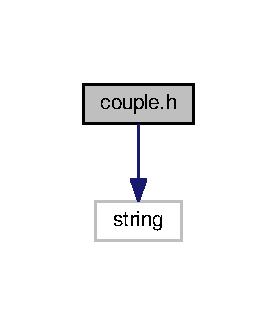
\includegraphics[width=133pt]{couple_8h__incl}
\end{center}
\end{figure}
This graph shows which files directly or indirectly include this file\+:
\nopagebreak
\begin{figure}[H]
\begin{center}
\leavevmode
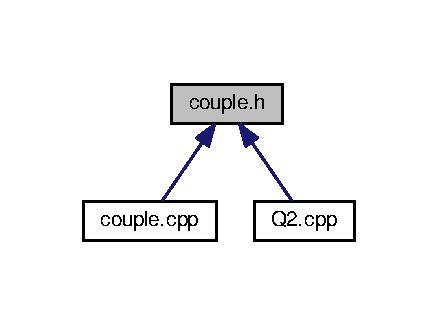
\includegraphics[width=350pt]{couple_8h__dep__incl}
\end{center}
\end{figure}
\subsection*{Classes}
\begin{DoxyCompactItemize}
\item 
class \hyperlink{classcouple}{couple}
\end{DoxyCompactItemize}

\hypertarget{couples_8txt}{}\section{couples.\+txt File Reference}
\label{couples_8txt}\index{couples.\+txt@{couples.\+txt}}

\hypertarget{gift_8cpp}{}\section{gift.\+cpp File Reference}
\label{gift_8cpp}\index{gift.\+cpp@{gift.\+cpp}}
{\ttfamily \#include \char`\"{}gift.\+h\char`\"{}}\\*
{\ttfamily \#include $<$string$>$}\\*
Include dependency graph for gift.\+cpp\+:
\nopagebreak
\begin{figure}[H]
\begin{center}
\leavevmode
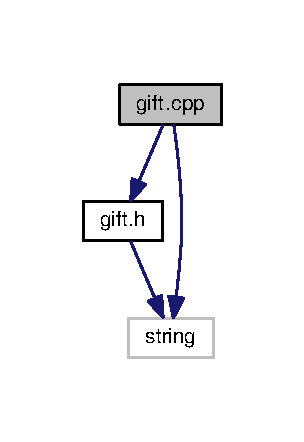
\includegraphics[width=146pt]{gift_8cpp__incl}
\end{center}
\end{figure}

\hypertarget{gift_8h}{}\section{gift.\+h File Reference}
\label{gift_8h}\index{gift.\+h@{gift.\+h}}
{\ttfamily \#include $<$string$>$}\\*
Include dependency graph for gift.\+h\+:
\nopagebreak
\begin{figure}[H]
\begin{center}
\leavevmode
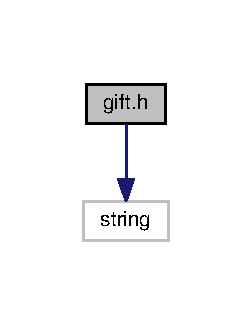
\includegraphics[width=121pt]{gift_8h__incl}
\end{center}
\end{figure}
This graph shows which files directly or indirectly include this file\+:
\nopagebreak
\begin{figure}[H]
\begin{center}
\leavevmode
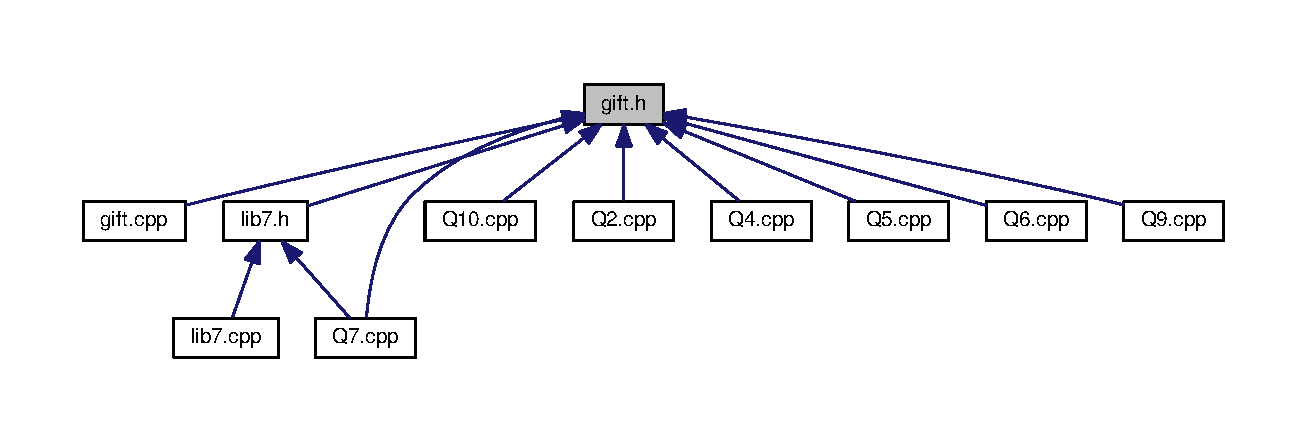
\includegraphics[width=195pt]{gift_8h__dep__incl}
\end{center}
\end{figure}
\subsection*{Classes}
\begin{DoxyCompactItemize}
\item 
class \hyperlink{classGift}{Gift}
\end{DoxyCompactItemize}

\hypertarget{gifts_8txt}{}\section{gifts.\+txt File Reference}
\label{gifts_8txt}\index{gifts.\+txt@{gifts.\+txt}}

\hypertarget{giftslog_8txt}{}\section{giftslog.\+txt File Reference}
\label{giftslog_8txt}\index{giftslog.\+txt@{giftslog.\+txt}}

\hypertarget{girl_8cpp}{}\section{girl.\+cpp File Reference}
\label{girl_8cpp}\index{girl.\+cpp@{girl.\+cpp}}
{\ttfamily \#include \char`\"{}girl.\+h\char`\"{}}\\*
{\ttfamily \#include $<$string$>$}\\*
Include dependency graph for girl.\+cpp\+:
\nopagebreak
\begin{figure}[H]
\begin{center}
\leavevmode
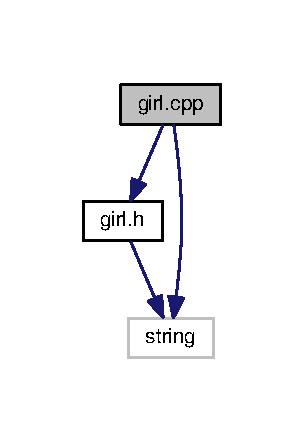
\includegraphics[width=146pt]{girl_8cpp__incl}
\end{center}
\end{figure}

\hypertarget{girl_8h}{}\section{girl.\+h File Reference}
\label{girl_8h}\index{girl.\+h@{girl.\+h}}
{\ttfamily \#include $<$string$>$}\\*
Include dependency graph for girl.\+h\+:
\nopagebreak
\begin{figure}[H]
\begin{center}
\leavevmode
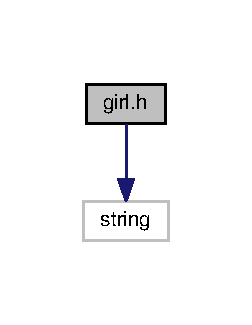
\includegraphics[width=121pt]{girl_8h__incl}
\end{center}
\end{figure}
This graph shows which files directly or indirectly include this file\+:
\nopagebreak
\begin{figure}[H]
\begin{center}
\leavevmode
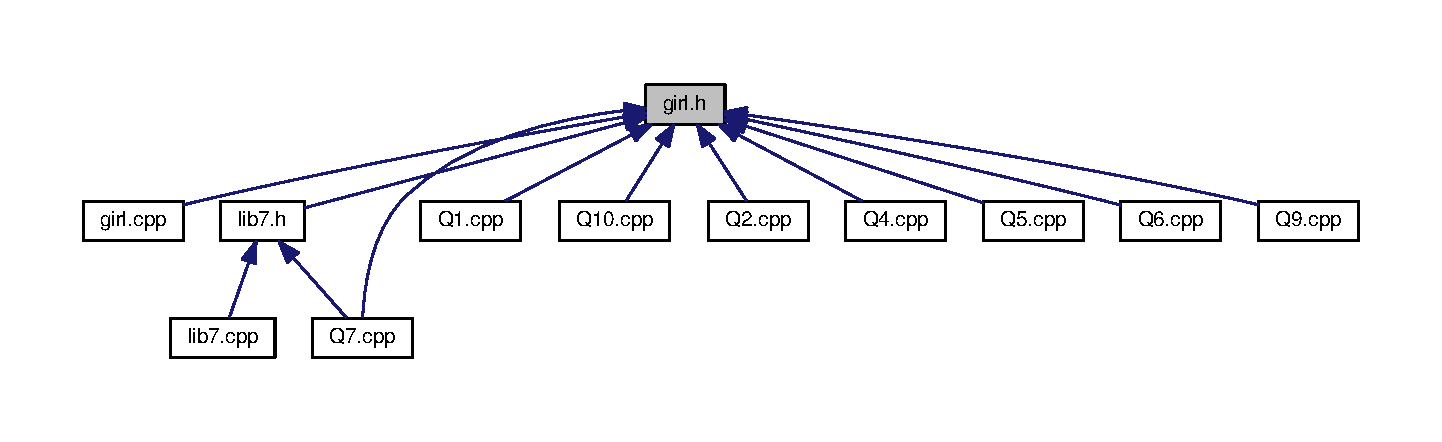
\includegraphics[width=350pt]{girl_8h__dep__incl}
\end{center}
\end{figure}
\subsection*{Classes}
\begin{DoxyCompactItemize}
\item 
class \hyperlink{classGirl}{Girl}
\end{DoxyCompactItemize}

\hypertarget{girlrec_8txt}{}\section{girlrec.\+txt File Reference}
\label{girlrec_8txt}\index{girlrec.\+txt@{girlrec.\+txt}}

\hypertarget{lib7_8cpp}{}\section{lib7.\+cpp File Reference}
\label{lib7_8cpp}\index{lib7.\+cpp@{lib7.\+cpp}}
{\ttfamily \#include \char`\"{}lib7.\+h\char`\"{}}\\*
Include dependency graph for lib7.\+cpp\+:
\nopagebreak
\begin{figure}[H]
\begin{center}
\leavevmode
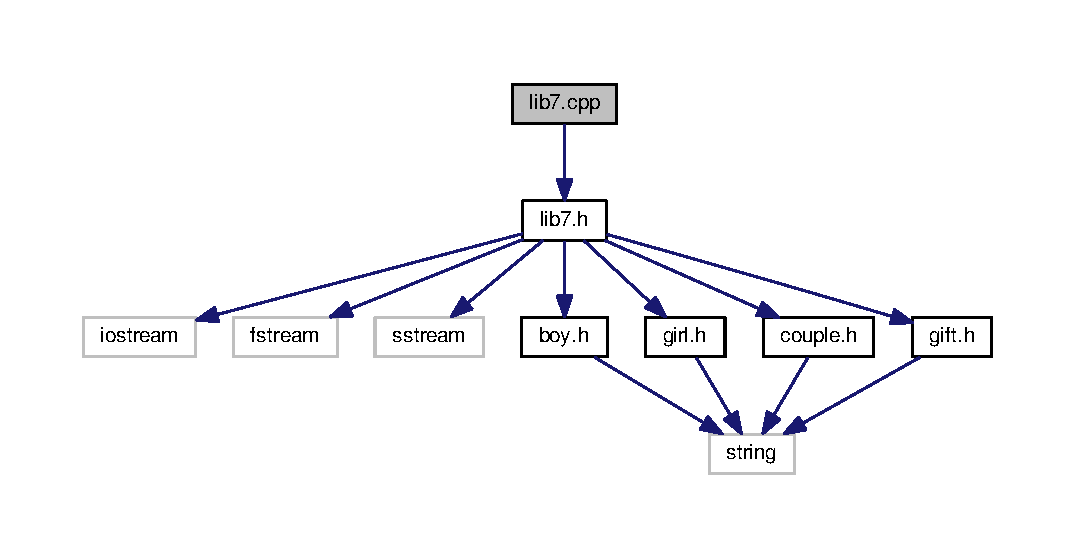
\includegraphics[width=350pt]{lib7_8cpp__incl}
\end{center}
\end{figure}

\hypertarget{lib7_8h}{}\section{lib7.\+h File Reference}
\label{lib7_8h}\index{lib7.\+h@{lib7.\+h}}
{\ttfamily \#include $<$iostream$>$}\\*
{\ttfamily \#include $<$fstream$>$}\\*
{\ttfamily \#include $<$sstream$>$}\\*
{\ttfamily \#include \char`\"{}boy.\+h\char`\"{}}\\*
{\ttfamily \#include \char`\"{}girl.\+h\char`\"{}}\\*
{\ttfamily \#include \char`\"{}couple.\+h\char`\"{}}\\*
{\ttfamily \#include \char`\"{}gift.\+h\char`\"{}}\\*
Include dependency graph for lib7.\+h\+:
\nopagebreak
\begin{figure}[H]
\begin{center}
\leavevmode
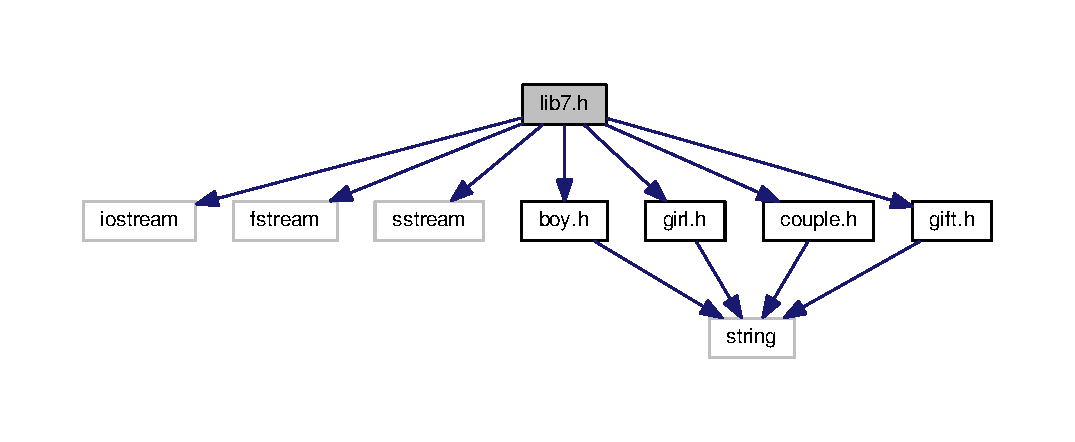
\includegraphics[width=350pt]{lib7_8h__incl}
\end{center}
\end{figure}
This graph shows which files directly or indirectly include this file\+:
\nopagebreak
\begin{figure}[H]
\begin{center}
\leavevmode
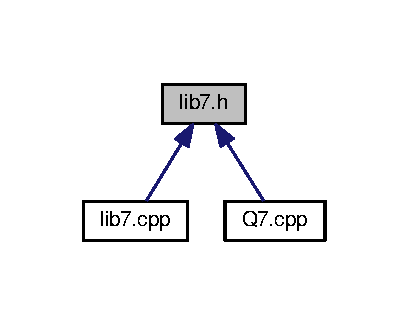
\includegraphics[width=196pt]{lib7_8h__dep__incl}
\end{center}
\end{figure}
\subsection*{Classes}
\begin{DoxyCompactItemize}
\item 
class \hyperlink{classLibrary}{Library}
\end{DoxyCompactItemize}
\subsection*{Variables}
\begin{DoxyCompactItemize}
\item 
int \hyperlink{lib7_8h_aeee5e31bf47987f4c471a1649ec9e43f}{no\+Boys} = 9
\item 
int \hyperlink{lib7_8h_afbf77341ebcfec44fd5ed146e13668bf}{no\+Girls} = 6
\item 
int \hyperlink{lib7_8h_a20a0f494ca2c397f664e1911db5e084b}{S} = 9
\item 
int \hyperlink{lib7_8h_a5464533d23b59ba11030432e73528730}{C} = 6
\end{DoxyCompactItemize}


\subsection{Variable Documentation}
\index{lib7.\+h@{lib7.\+h}!C@{C}}
\index{C@{C}!lib7.\+h@{lib7.\+h}}
\subsubsection[{\texorpdfstring{C}{C}}]{\setlength{\rightskip}{0pt plus 5cm}int C = 6}\hypertarget{lib7_8h_a5464533d23b59ba11030432e73528730}{}\label{lib7_8h_a5464533d23b59ba11030432e73528730}
\index{lib7.\+h@{lib7.\+h}!no\+Boys@{no\+Boys}}
\index{no\+Boys@{no\+Boys}!lib7.\+h@{lib7.\+h}}
\subsubsection[{\texorpdfstring{no\+Boys}{noBoys}}]{\setlength{\rightskip}{0pt plus 5cm}int no\+Boys = 9}\hypertarget{lib7_8h_aeee5e31bf47987f4c471a1649ec9e43f}{}\label{lib7_8h_aeee5e31bf47987f4c471a1649ec9e43f}
\index{lib7.\+h@{lib7.\+h}!no\+Girls@{no\+Girls}}
\index{no\+Girls@{no\+Girls}!lib7.\+h@{lib7.\+h}}
\subsubsection[{\texorpdfstring{no\+Girls}{noGirls}}]{\setlength{\rightskip}{0pt plus 5cm}int no\+Girls = 6}\hypertarget{lib7_8h_afbf77341ebcfec44fd5ed146e13668bf}{}\label{lib7_8h_afbf77341ebcfec44fd5ed146e13668bf}
\index{lib7.\+h@{lib7.\+h}!S@{S}}
\index{S@{S}!lib7.\+h@{lib7.\+h}}
\subsubsection[{\texorpdfstring{S}{S}}]{\setlength{\rightskip}{0pt plus 5cm}int S = 9}\hypertarget{lib7_8h_a20a0f494ca2c397f664e1911db5e084b}{}\label{lib7_8h_a20a0f494ca2c397f664e1911db5e084b}

\hypertarget{logfile7_8txt}{}\section{logfile7.\+txt File Reference}
\label{logfile7_8txt}\index{logfile7.\+txt@{logfile7.\+txt}}

\hypertarget{logfile8_8txt}{}\section{logfile8.\+txt File Reference}
\label{logfile8_8txt}\index{logfile8.\+txt@{logfile8.\+txt}}

\hypertarget{output_8txt}{}\section{output.\+txt File Reference}
\label{output_8txt}\index{output.\+txt@{output.\+txt}}

\hypertarget{Q1_8cpp}{}\section{Q1.\+cpp File Reference}
\label{Q1_8cpp}\index{Q1.\+cpp@{Q1.\+cpp}}
{\ttfamily \#include $<$iostream$>$}\\*
{\ttfamily \#include $<$fstream$>$}\\*
{\ttfamily \#include $<$string$>$}\\*
{\ttfamily \#include \char`\"{}boy.\+h\char`\"{}}\\*
{\ttfamily \#include \char`\"{}girl.\+h\char`\"{}}\\*
Include dependency graph for Q1.\+cpp\+:
\nopagebreak
\begin{figure}[H]
\begin{center}
\leavevmode
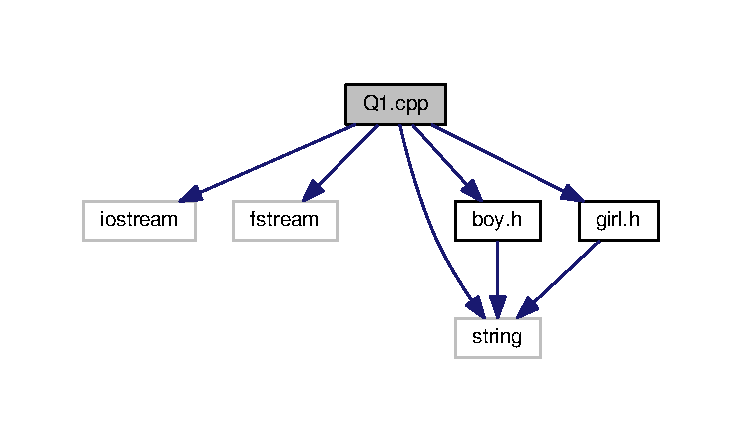
\includegraphics[width=350pt]{Q1_8cpp__incl}
\end{center}
\end{figure}
\subsection*{Functions}
\begin{DoxyCompactItemize}
\item 
int \hyperlink{Q1_8cpp_ae66f6b31b5ad750f1fe042a706a4e3d4}{main} ()
\end{DoxyCompactItemize}


\subsection{Function Documentation}
\index{Q1.\+cpp@{Q1.\+cpp}!main@{main}}
\index{main@{main}!Q1.\+cpp@{Q1.\+cpp}}
\subsubsection[{\texorpdfstring{main()}{main()}}]{\setlength{\rightskip}{0pt plus 5cm}int main (
\begin{DoxyParamCaption}
{}
\end{DoxyParamCaption}
)}\hypertarget{Q1_8cpp_ae66f6b31b5ad750f1fe042a706a4e3d4}{}\label{Q1_8cpp_ae66f6b31b5ad750f1fe042a706a4e3d4}
$<$ Read boys data

$<$ Make Couples 
\begin{DoxyCode}
10 \{
11     ifstream boyPtr(\textcolor{stringliteral}{"boyrec.txt"}, ios::in);
12     ifstream girlPtr(\textcolor{stringliteral}{"girlrec.txt"}, ios::in);
13     ofstream opPtr(\textcolor{stringliteral}{"output.txt"}, ios::out);
14     \textcolor{keywordtype}{int} \hyperlink{lib7_8h_aeee5e31bf47987f4c471a1649ec9e43f}{noBoys} = 7,\hyperlink{lib7_8h_afbf77341ebcfec44fd5ed146e13668bf}{noGirls} = 4;
15     \hyperlink{classBoy}{Boy} boy[\hyperlink{lib7_8h_aeee5e31bf47987f4c471a1649ec9e43f}{noBoys}];
16     \hyperlink{classGirl}{Girl} girl[\hyperlink{lib7_8h_afbf77341ebcfec44fd5ed146e13668bf}{noGirls}];
17     \textcolor{keywordtype}{int} maint, budget,intelli,attr,i;
18     \textcolor{keywordtype}{string} name,girlName,boyName,type;
19     
21     \textcolor{keywordflow}{for}( i = 0; i < \hyperlink{lib7_8h_aeee5e31bf47987f4c471a1649ec9e43f}{noBoys}; i++) \{
22         boyPtr >> name >> type >> attr >> intelli >> budget ;
23         boy[i].\hyperlink{classBoy_aa6d16a472a01b4e7da0817fe94d9a2bd}{init}(name,type,attr,intelli,budget);
24     \}
25 
27     \textcolor{keywordflow}{for}( i = 0; i < \hyperlink{lib7_8h_afbf77341ebcfec44fd5ed146e13668bf}{noGirls}; i++) \{
28         girlPtr >> name >> type >> attr >> intelli >> maint ;
29         girl[i].\hyperlink{classGirl_aba849734c908a23bde2e5bd9c335c450}{init}(name,type,attr,intelli,budget);
30     \}
31 
32     \textcolor{keywordtype}{int} j = 0,k = 0;
34     \textcolor{keywordflow}{for}( i = 0; i < \hyperlink{lib7_8h_afbf77341ebcfec44fd5ed146e13668bf}{noGirls}; i++) \{
35         maint = girl[i].\hyperlink{classGirl_ac23543169a5e339a3c93fbd8aeb977ca}{getMaint}();
36         girlName = girl[i].\hyperlink{classGirl_a27a705fb94b92dfd6929d0bf4bcaf5e1}{getName}();
37         \textcolor{keywordflow}{for}( j = k; j < \hyperlink{lib7_8h_aeee5e31bf47987f4c471a1649ec9e43f}{noBoys}; j++) \{
38             budget = boy[j].\hyperlink{classBoy_a05c48b12091ebcad44ba86ba88514ac5}{getBudget}();
39             boyName = boy[j].\hyperlink{classBoy_acf59fd0074a6ea3413751a95b2970303}{getName}();
40             \textcolor{keywordflow}{if}(maint < budget && !(girl[i].getStatus() ) && !(boy[j].getStatus() ) ) \{
41                     opPtr << girlName << \textcolor{stringliteral}{"        "} << boyName << endl;
42                     girl[i].\hyperlink{classGirl_ac4e040efdf40d12044bda1b647e0d2da}{changeStatus}();
43                     boy[j].\hyperlink{classBoy_a2a8cc82d9332c07eb475198e46028d52}{changeStatus}();
44                     k++;
45                     \textcolor{keywordflow}{break};
46             \} \textcolor{keywordflow}{else} \{
47                 j--;
48             \}
49         \}
50     \}
51 \}
\end{DoxyCode}

\hypertarget{Q10_8cpp}{}\section{Q10.\+cpp File Reference}
\label{Q10_8cpp}\index{Q10.\+cpp@{Q10.\+cpp}}
{\ttfamily \#include $<$iostream$>$}\\*
{\ttfamily \#include $<$fstream$>$}\\*
{\ttfamily \#include $<$sstream$>$}\\*
{\ttfamily \#include $<$cmath$>$}\\*
{\ttfamily \#include \char`\"{}boy.\+h\char`\"{}}\\*
{\ttfamily \#include \char`\"{}girl.\+h\char`\"{}}\\*
{\ttfamily \#include \char`\"{}couple.\+h\char`\"{}}\\*
{\ttfamily \#include \char`\"{}gift.\+h\char`\"{}}\\*
Include dependency graph for Q10.\+cpp\+:
\nopagebreak
\begin{figure}[H]
\begin{center}
\leavevmode
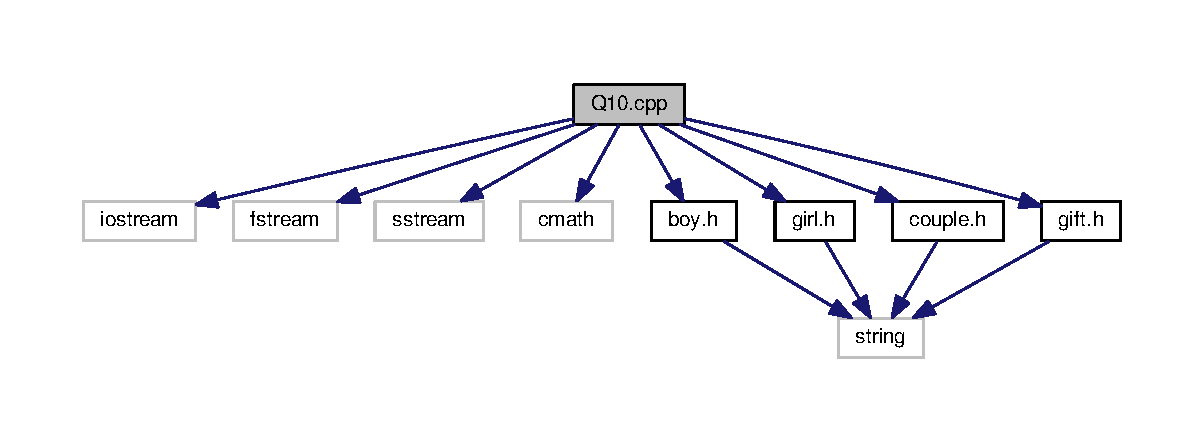
\includegraphics[width=350pt]{Q10_8cpp__incl}
\end{center}
\end{figure}
\subsection*{Macros}
\begin{DoxyCompactItemize}
\item 
\#define \hyperlink{Q10_8cpp_a111da81ae5883147168bbb8366377b10}{B}~9
\item 
\#define \hyperlink{Q10_8cpp_aed9ea78689ecce0b7264c02c7f8a9a54}{G}~5
\item 
\#define \hyperlink{Q10_8cpp_ac4cf4b2ab929bd23951a8676eeac086b}{C}~5
\item 
\#define \hyperlink{Q10_8cpp_a5e0c07e523d4e77a2cafca06feb836f6}{Gf}~15
\item 
\#define \hyperlink{Q10_8cpp_a97d832ae23af4f215e801e37e4f94254}{K}~2
\end{DoxyCompactItemize}
\subsection*{Functions}
\begin{DoxyCompactItemize}
\item 
void \hyperlink{Q10_8cpp_ac75f5851dc71925a5c837c0b35a51d26}{swap} (\hyperlink{classGift}{Gift} \&a, \hyperlink{classGift}{Gift} \&b)
\item 
void \hyperlink{Q10_8cpp_a9ed5e5ebda90f206f83cd424ebebe79d}{swapC} (Couple \&a, Couple \&b)
\item 
{\footnotesize template$<$class T $>$ }\\void \hyperlink{Q10_8cpp_afb2bbadfe7cfd2620d67ca6d0ccb2411}{sorting\+Datastructure} (\hyperlink{Q6_8cpp_a0acb682b8260ab1c60b918599864e2e5}{T} $\ast$arr, int n, int k, string s)
\item 
int \hyperlink{Q10_8cpp_ae66f6b31b5ad750f1fe042a706a4e3d4}{main} ()
\end{DoxyCompactItemize}


\subsection{Macro Definition Documentation}
\index{Q10.\+cpp@{Q10.\+cpp}!B@{B}}
\index{B@{B}!Q10.\+cpp@{Q10.\+cpp}}
\subsubsection[{\texorpdfstring{B}{B}}]{\setlength{\rightskip}{0pt plus 5cm}\#define B~9}\hypertarget{Q10_8cpp_a111da81ae5883147168bbb8366377b10}{}\label{Q10_8cpp_a111da81ae5883147168bbb8366377b10}
\index{Q10.\+cpp@{Q10.\+cpp}!C@{C}}
\index{C@{C}!Q10.\+cpp@{Q10.\+cpp}}
\subsubsection[{\texorpdfstring{C}{C}}]{\setlength{\rightskip}{0pt plus 5cm}\#define C~5}\hypertarget{Q10_8cpp_ac4cf4b2ab929bd23951a8676eeac086b}{}\label{Q10_8cpp_ac4cf4b2ab929bd23951a8676eeac086b}
\index{Q10.\+cpp@{Q10.\+cpp}!G@{G}}
\index{G@{G}!Q10.\+cpp@{Q10.\+cpp}}
\subsubsection[{\texorpdfstring{G}{G}}]{\setlength{\rightskip}{0pt plus 5cm}\#define G~5}\hypertarget{Q10_8cpp_aed9ea78689ecce0b7264c02c7f8a9a54}{}\label{Q10_8cpp_aed9ea78689ecce0b7264c02c7f8a9a54}
\index{Q10.\+cpp@{Q10.\+cpp}!Gf@{Gf}}
\index{Gf@{Gf}!Q10.\+cpp@{Q10.\+cpp}}
\subsubsection[{\texorpdfstring{Gf}{Gf}}]{\setlength{\rightskip}{0pt plus 5cm}\#define Gf~15}\hypertarget{Q10_8cpp_a5e0c07e523d4e77a2cafca06feb836f6}{}\label{Q10_8cpp_a5e0c07e523d4e77a2cafca06feb836f6}
\index{Q10.\+cpp@{Q10.\+cpp}!K@{K}}
\index{K@{K}!Q10.\+cpp@{Q10.\+cpp}}
\subsubsection[{\texorpdfstring{K}{K}}]{\setlength{\rightskip}{0pt plus 5cm}\#define K~2}\hypertarget{Q10_8cpp_a97d832ae23af4f215e801e37e4f94254}{}\label{Q10_8cpp_a97d832ae23af4f215e801e37e4f94254}


\subsection{Function Documentation}
\index{Q10.\+cpp@{Q10.\+cpp}!main@{main}}
\index{main@{main}!Q10.\+cpp@{Q10.\+cpp}}
\subsubsection[{\texorpdfstring{main()}{main()}}]{\setlength{\rightskip}{0pt plus 5cm}int main (
\begin{DoxyParamCaption}
{}
\end{DoxyParamCaption}
)}\hypertarget{Q10_8cpp_ae66f6b31b5ad750f1fe042a706a4e3d4}{}\label{Q10_8cpp_ae66f6b31b5ad750f1fe042a706a4e3d4}
$<$ Read boys data

$<$ Read the gifts

$<$ Sort couples according to their happiness

$<$ Print sorted couple in a file 
\begin{DoxyCode}
51 \{
52     ifstream boyPtr(\textcolor{stringliteral}{"boyrec.txt"}, ios::in);
53     ifstream girlPtr(\textcolor{stringliteral}{"girlrec.txt"}, ios::in);
54     ofstream opPtr(\textcolor{stringliteral}{"output.txt"}, ios::out);
55     ifstream giftPtr(\textcolor{stringliteral}{"gifts.txt"}, ios::in);
56     ofstream giftout(\textcolor{stringliteral}{"giftslog.txt"}, ios::out);
57 
58     \textcolor{keywordtype}{int} \hyperlink{lib7_8h_aeee5e31bf47987f4c471a1649ec9e43f}{noBoys} = 9,\hyperlink{lib7_8h_afbf77341ebcfec44fd5ed146e13668bf}{noGirls} = 6;
59     \hyperlink{classBoy}{Boy} boy[\hyperlink{lib7_8h_aeee5e31bf47987f4c471a1649ec9e43f}{noBoys}];
60     \hyperlink{classGirl}{Girl} girl[\hyperlink{lib7_8h_afbf77341ebcfec44fd5ed146e13668bf}{noGirls}];
61     \hyperlink{classcouple}{couple} \hyperlink{classcouple}{couple}[\hyperlink{lib7_8h_afbf77341ebcfec44fd5ed146e13668bf}{noGirls}];
62     \hyperlink{classGift}{Gift} gift[4*\hyperlink{lib7_8h_afbf77341ebcfec44fd5ed146e13668bf}{noGirls}];
63     \textcolor{keywordtype}{int} maint, budget,intelli,attr,i;
64     \textcolor{keywordtype}{string} name,girlName,boyName,type;
65     
67     \textcolor{keywordflow}{for}( i = 0; i < \hyperlink{lib7_8h_aeee5e31bf47987f4c471a1649ec9e43f}{noBoys}; i++) \{
68         boyPtr >> name >> type >>attr >> intelli >> budget ;
69         boy[i].\hyperlink{classBoy_aa6d16a472a01b4e7da0817fe94d9a2bd}{init}(name,type,attr,intelli,budget);
70     \}
71 
73     \textcolor{keywordflow}{for}( i = 0; i < \hyperlink{lib7_8h_afbf77341ebcfec44fd5ed146e13668bf}{noGirls}; i++) \{
74         girlPtr >> name >> type >> attr >> intelli >> maint ;
75         girl[i].\hyperlink{classGirl_aba849734c908a23bde2e5bd9c335c450}{init}(name,type,attr,intelli,budget);
76     \}
77 
79     \textcolor{keywordtype}{int} j = 0,k = 0,ind = 0;
80     \textcolor{keywordflow}{for}( i = 0; i < \hyperlink{lib7_8h_afbf77341ebcfec44fd5ed146e13668bf}{noGirls}; i++) \{
81         maint = girl[i].\hyperlink{classGirl_ac23543169a5e339a3c93fbd8aeb977ca}{getMaint}();
82         girlName = girl[i].\hyperlink{classGirl_a27a705fb94b92dfd6929d0bf4bcaf5e1}{getName}();
83         \textcolor{keywordflow}{for}( j = k; j < \hyperlink{lib7_8h_aeee5e31bf47987f4c471a1649ec9e43f}{noBoys}; j++) \{
84             budget = boy[j].\hyperlink{classBoy_a05c48b12091ebcad44ba86ba88514ac5}{getBudget}();
85             boyName = boy[j].\hyperlink{classBoy_acf59fd0074a6ea3413751a95b2970303}{getName}();
86             \textcolor{keywordflow}{if}(maint < budget && !(girl[i].getStatus() ) && !(boy[j].getStatus() ) ) \{
87                     opPtr << girlName << \textcolor{stringliteral}{"        "} << boyName << endl;
88                     couple[i].\hyperlink{classcouple_a3ee36a530603865ff58470bae84da220}{init}(boyName,boy[j].getType(), girlName,boy[j].getBudget(),girl[i].
      getMaint(),boy[j].getAttr(),girl[i].getAttr(),boy[j].getIntelli(),girl[i].getIntelli());
89                     girl[i].\hyperlink{classGirl_ac4e040efdf40d12044bda1b647e0d2da}{changeStatus}();
90                     boy[j].\hyperlink{classBoy_a2a8cc82d9332c07eb475198e46028d52}{changeStatus}();
91                     k++;
92                     \textcolor{keywordflow}{break};
93             \} \textcolor{keywordflow}{else} \{
94                 j--;
95             \}
96         \}
97     \}
98 
99     \textcolor{keywordtype}{int} val,pr;
100     std:: string ty;
102     \textcolor{keywordflow}{for}(i = 0; i < 14; i++) \{
103         giftPtr >> val >> pr >> ty;
104         gift[i].\hyperlink{classGift_aee7c5672f4d1ee738a7dbeb6f952fe1f}{init}(val,pr,ty);
105     \}
107     \textcolor{keywordtype}{int} currbud;
108     j = 0;
109     \textcolor{keywordflow}{for}(i = 0; i < \hyperlink{lib7_8h_afbf77341ebcfec44fd5ed146e13668bf}{noGirls}; i++) \{
110         currbud = couple[i].\hyperlink{classcouple_af4b090a72111d7ba566747e4e305a6ec}{getCurrBudget}() ;
111         \textcolor{keywordflow}{while}(currbud > gift[j].getPrice() && j < 14) \{
112             pr = gift[j].\hyperlink{classGift_aa114ca9629b5f02e4df6731d33c69373}{getPrice}();
113             giftout << couple[i].\hyperlink{classcouple_afe07f86e775d20508e6cd139488af366}{getBoyname}() << \textcolor{stringliteral}{"  "} << couple[i].
      \hyperlink{classcouple_a7897320b780dbeaa85380c71803de9c2}{getGirlname}() << \textcolor{stringliteral}{"  "} <<  pr << endl;
114             couple[i].\hyperlink{classcouple_afa9889ca750dd53ffd06daf78cbee326}{changeCurrBudget}(pr);
115             j++;
116             currbud = couple[i].\hyperlink{classcouple_af4b090a72111d7ba566747e4e305a6ec}{getCurrBudget}() ;
117         \}
118     \}
119     \textcolor{comment}{/*}
120 \textcolor{comment}{    * Calculate Happiness of Girls
}
121 \textcolor{comment}{    */}
122     \textcolor{keywordtype}{int} bh,gh,cost;
123     \textcolor{keywordflow}{for}( i = 0; i< \hyperlink{lib7_8h_afbf77341ebcfec44fd5ed146e13668bf}{noGirls}; i++) \{
124         type = girl[i].\hyperlink{classGirl_a2b5bbd35287b7aa074f39702b564bc97}{getType}();
125         cost = couple[i].\hyperlink{classcouple_a5f31ac8019f5db29694dc36cdba958b8}{getCost}();
126         \textcolor{keywordflow}{if}(type == \textcolor{stringliteral}{"Choosy"}) \{
127             gh = log10(cost / girl[i].getMaint());
128         \} \textcolor{keywordflow}{else} \textcolor{keywordflow}{if}(type == \textcolor{stringliteral}{"Normal"}) \{
129             gh = cost / girl[i].\hyperlink{classGirl_ac23543169a5e339a3c93fbd8aeb977ca}{getMaint}();
130         \} \textcolor{keywordflow}{else} \textcolor{keywordflow}{if}(type == \textcolor{stringliteral}{"Desperate"}) \{
131             gh = exp(cost / girl[i].getMaint());
132         \}
133         couple[i].\hyperlink{classcouple_a526f48a752f261212d111a630f5730f4}{setGirlHappiness}(gh);
134     \}
135  
137     \textcolor{keywordflow}{for}(i = 0; i < \hyperlink{lib7_8h_afbf77341ebcfec44fd5ed146e13668bf}{noGirls}; i++) \{
138         type = couple[i].\hyperlink{classcouple_a687986a266cc984fa5d2114c888f52cf}{getBoyType}();
139         cost = couple[i].\hyperlink{classcouple_a5f31ac8019f5db29694dc36cdba958b8}{getCost}();
140         \textcolor{keywordflow}{if}(type == \textcolor{stringliteral}{"Miser"}) \{
141             bh = couple[i].\hyperlink{classcouple_a92496b42f9d1392013c4d7456318ad70}{getBudget}() - cost;
142         \} \textcolor{keywordflow}{else} \textcolor{keywordflow}{if}(type == \textcolor{stringliteral}{"Generous"}) \{
143             bh = couple[i].\hyperlink{classcouple_ada2f9b79cede186a0e9bcd6b48bec804}{getGirlHappiness}();
144         \} \textcolor{keywordflow}{else} \{
145             bh = girl[i].\hyperlink{classGirl_afe73c4c4f180aa8f5e0bc4f87455ec0b}{getIntelligence}();
146         \}
147         couple[i].\hyperlink{classcouple_a50a890cb7ffd3a44f0201b8e0d84f744}{setBoyHappiness}(bh);
148         couple[i].\hyperlink{classcouple_aaaadc39a9f265907581925ef579c7214}{setHappiness}();
149     \}
150 
151     \textcolor{keywordtype}{int} h1,h2;
152 
153     k = 3;
155     \textcolor{keywordflow}{for}(i = 0; i < \hyperlink{lib7_8h_afbf77341ebcfec44fd5ed146e13668bf}{noGirls}; i++) \{
156         h1 = couple[i].\hyperlink{classcouple_a31d0a1c8acff06a64ebc2e2f6d9a68b1}{getHappiness}();
157         \textcolor{keywordflow}{for}(j = i+1; j < \hyperlink{lib7_8h_afbf77341ebcfec44fd5ed146e13668bf}{noGirls}; j++) \{
158             h2 = couple[j].\hyperlink{classcouple_a31d0a1c8acff06a64ebc2e2f6d9a68b1}{getHappiness}();
159             \textcolor{keywordflow}{if}(h1 > h2) \{
160                 \hyperlink{Q2_8cpp_a5a408068bacb1c7add72673eb9d96bbc}{swapCouple}(couple[i], couple[j]);
161             \}
162         \}
163     \}
164 
165     ofstream happiness(\textcolor{stringliteral}{"sortedHappiness.txt"}, ios::out);
166     ofstream compatibility(\textcolor{stringliteral}{"sortedComaptibility.txt"}, ios::out);
167 
169     \textcolor{keywordflow}{for}(i = 0; i< k; i++) \{
170         happiness << couple[i].\hyperlink{classcouple_afe07f86e775d20508e6cd139488af366}{getBoyname}() << \textcolor{stringliteral}{"  "} << couple[i].
      \hyperlink{classcouple_a7897320b780dbeaa85380c71803de9c2}{getGirlname}() <<  \textcolor{stringliteral}{"   "} << couple[i].\hyperlink{classcouple_a31d0a1c8acff06a64ebc2e2f6d9a68b1}{getHappiness}() << endl;
171     \}
172 
174     \textcolor{keywordflow}{for}( i = 0; i < \hyperlink{lib7_8h_afbf77341ebcfec44fd5ed146e13668bf}{noGirls}; i++) \{
175         couple[i].\hyperlink{classcouple_a91bc77488fe8b5d30643b9ff0a56d359}{setCompatibility}();
176     \}
177 
179     \textcolor{keywordflow}{for}(i = 0; i < \hyperlink{lib7_8h_afbf77341ebcfec44fd5ed146e13668bf}{noGirls}; i++) \{
180         h1 = couple[i].\hyperlink{classcouple_a43d2852ce692307280ba9ab2366c16eb}{getCompatibility}();
181         \textcolor{keywordflow}{for}(j = i+1; j < \hyperlink{lib7_8h_afbf77341ebcfec44fd5ed146e13668bf}{noGirls}; j++) \{
182             h2 = couple[j].\hyperlink{classcouple_a43d2852ce692307280ba9ab2366c16eb}{getCompatibility}();
183             \textcolor{keywordflow}{if}(h1 > h2) \{
184                 \hyperlink{Q10_8cpp_a9ed5e5ebda90f206f83cd424ebebe79d}{swapC}(couple[i],couple[j]);
185             \}
186         \}
187     \}
188 
190     \textcolor{keywordflow}{for}(i = 0; i< k; i++) \{
191         compatibility << couple[i].\hyperlink{classcouple_afe07f86e775d20508e6cd139488af366}{getBoyname}() << \textcolor{stringliteral}{"  "} << couple[i].
      \hyperlink{classcouple_a7897320b780dbeaa85380c71803de9c2}{getGirlname}() << endl;
192     \}
193 
194 \}
\end{DoxyCode}
\index{Q10.\+cpp@{Q10.\+cpp}!sorting\+Datastructure@{sorting\+Datastructure}}
\index{sorting\+Datastructure@{sorting\+Datastructure}!Q10.\+cpp@{Q10.\+cpp}}
\subsubsection[{\texorpdfstring{sorting\+Datastructure(\+T $\ast$arr, int n, int k, string s)}{sortingDatastructure(T *arr, int n, int k, string s)}}]{\setlength{\rightskip}{0pt plus 5cm}template$<$class T $>$ void sorting\+Datastructure (
\begin{DoxyParamCaption}
\item[{{\bf T} $\ast$}]{arr, }
\item[{int}]{n, }
\item[{int}]{k, }
\item[{string}]{s}
\end{DoxyParamCaption}
)}\hypertarget{Q10_8cpp_afb2bbadfe7cfd2620d67ca6d0ccb2411}{}\label{Q10_8cpp_afb2bbadfe7cfd2620d67ca6d0ccb2411}

\begin{DoxyCode}
37 \{
38     \textcolor{keywordflow}{for}(\textcolor{keywordtype}{int} i = 0  ; i< n-1; i++) \{
39         \textcolor{keywordflow}{for}(\textcolor{keywordtype}{int} j = i+1; j < n; j++) \{
40              \textcolor{keywordflow}{if}(s == \textcolor{stringliteral}{"attractiveness"}) \{
41                 \textcolor{keywordflow}{if}(arr[j].getAttractiveness() < arr[i].getAttractiveness()) \{
42                     \hyperlink{Q10_8cpp_ac75f5851dc71925a5c837c0b35a51d26}{swap}(arr[j],arr[i]);
43                 \}
44             \}
45         \}
46     \}
47 \}
\end{DoxyCode}
\index{Q10.\+cpp@{Q10.\+cpp}!swap@{swap}}
\index{swap@{swap}!Q10.\+cpp@{Q10.\+cpp}}
\subsubsection[{\texorpdfstring{swap(\+Gift \&a, Gift \&b)}{swap(Gift &a, Gift &b)}}]{\setlength{\rightskip}{0pt plus 5cm}void Gift\+Allocation\+::swap (
\begin{DoxyParamCaption}
\item[{{\bf Gift} \&}]{a, }
\item[{{\bf Gift} \&}]{b}
\end{DoxyParamCaption}
)}\hypertarget{Q10_8cpp_ac75f5851dc71925a5c837c0b35a51d26}{}\label{Q10_8cpp_ac75f5851dc71925a5c837c0b35a51d26}

\begin{DoxyCode}
21 \{
22     \hyperlink{classGift}{Gift} temp = a;
23     a = b;
24     b = temp;
25 \}
\end{DoxyCode}
\index{Q10.\+cpp@{Q10.\+cpp}!swapC@{swapC}}
\index{swapC@{swapC}!Q10.\+cpp@{Q10.\+cpp}}
\subsubsection[{\texorpdfstring{swap\+C(\+Couple \&a, Couple \&b)}{swapC(Couple &a, Couple &b)}}]{\setlength{\rightskip}{0pt plus 5cm}void swapC (
\begin{DoxyParamCaption}
\item[{Couple \&}]{a, }
\item[{Couple \&}]{b}
\end{DoxyParamCaption}
)}\hypertarget{Q10_8cpp_a9ed5e5ebda90f206f83cd424ebebe79d}{}\label{Q10_8cpp_a9ed5e5ebda90f206f83cd424ebebe79d}

\begin{DoxyCode}
28 \{
29     Couple temp = a;
30     a = b;
31     b = temp;
32 \}
\end{DoxyCode}

\hypertarget{Q2_8cpp}{}\section{Q2.\+cpp File Reference}
\label{Q2_8cpp}\index{Q2.\+cpp@{Q2.\+cpp}}
{\ttfamily \#include $<$iostream$>$}\\*
{\ttfamily \#include $<$fstream$>$}\\*
{\ttfamily \#include $<$string$>$}\\*
{\ttfamily \#include \char`\"{}boy.\+h\char`\"{}}\\*
{\ttfamily \#include \char`\"{}girl.\+h\char`\"{}}\\*
{\ttfamily \#include \char`\"{}couple.\+h\char`\"{}}\\*
{\ttfamily \#include \char`\"{}gift.\+h\char`\"{}}\\*
{\ttfamily \#include $<$cmath$>$}\\*
Include dependency graph for Q2.\+cpp\+:
\nopagebreak
\begin{figure}[H]
\begin{center}
\leavevmode
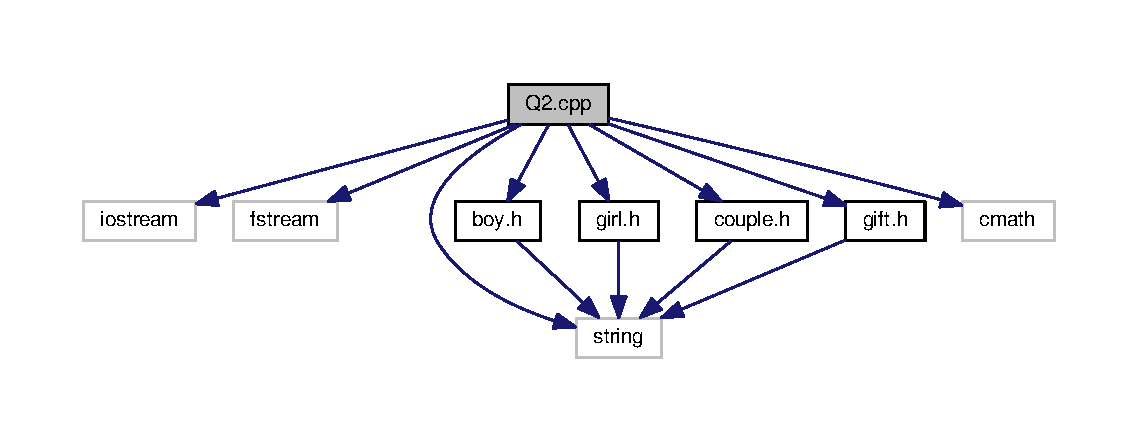
\includegraphics[width=350pt]{Q2_8cpp__incl}
\end{center}
\end{figure}
\subsection*{Functions}
\begin{DoxyCompactItemize}
\item 
void \hyperlink{Q2_8cpp_a5a408068bacb1c7add72673eb9d96bbc}{swap\+Couple} (\hyperlink{classcouple}{couple} \&a, \hyperlink{classcouple}{couple} \&b)
\item 
void \hyperlink{Q2_8cpp_ac5c65f5b5ec33f7b8ab8012de336fdb7}{swapC} (\hyperlink{classcouple}{couple} \&a, \hyperlink{classcouple}{couple} \&b)
\item 
int \hyperlink{Q2_8cpp_ae66f6b31b5ad750f1fe042a706a4e3d4}{main} ()
\end{DoxyCompactItemize}


\subsection{Function Documentation}
\index{Q2.\+cpp@{Q2.\+cpp}!main@{main}}
\index{main@{main}!Q2.\+cpp@{Q2.\+cpp}}
\subsubsection[{\texorpdfstring{main()}{main()}}]{\setlength{\rightskip}{0pt plus 5cm}int main (
\begin{DoxyParamCaption}
{}
\end{DoxyParamCaption}
)}\hypertarget{Q2_8cpp_ae66f6b31b5ad750f1fe042a706a4e3d4}{}\label{Q2_8cpp_ae66f6b31b5ad750f1fe042a706a4e3d4}
$<$ Read boys data

$<$ Read the gifts

$<$ Sort couples according to their happiness

$<$ Print sorted couple in a file \index{Q2.\+cpp@{Q2.\+cpp}!swapC@{swapC}}
\index{swapC@{swapC}!Q2.\+cpp@{Q2.\+cpp}}
\subsubsection[{\texorpdfstring{swap\+C(couple \&a, couple \&b)}{swapC(couple &a, couple &b)}}]{\setlength{\rightskip}{0pt plus 5cm}void swapC (
\begin{DoxyParamCaption}
\item[{{\bf couple} \&}]{a, }
\item[{{\bf couple} \&}]{b}
\end{DoxyParamCaption}
)}\hypertarget{Q2_8cpp_ac5c65f5b5ec33f7b8ab8012de336fdb7}{}\label{Q2_8cpp_ac5c65f5b5ec33f7b8ab8012de336fdb7}
\index{Q2.\+cpp@{Q2.\+cpp}!swap\+Couple@{swap\+Couple}}
\index{swap\+Couple@{swap\+Couple}!Q2.\+cpp@{Q2.\+cpp}}
\subsubsection[{\texorpdfstring{swap\+Couple(couple \&a, couple \&b)}{swapCouple(couple &a, couple &b)}}]{\setlength{\rightskip}{0pt plus 5cm}void swap\+Couple (
\begin{DoxyParamCaption}
\item[{{\bf couple} \&}]{a, }
\item[{{\bf couple} \&}]{b}
\end{DoxyParamCaption}
)}\hypertarget{Q2_8cpp_a5a408068bacb1c7add72673eb9d96bbc}{}\label{Q2_8cpp_a5a408068bacb1c7add72673eb9d96bbc}

\hypertarget{Q4_8cpp}{}\section{Q4.\+cpp File Reference}
\label{Q4_8cpp}\index{Q4.\+cpp@{Q4.\+cpp}}
{\ttfamily \#include $<$iostream$>$}\\*
{\ttfamily \#include $<$fstream$>$}\\*
{\ttfamily \#include $<$string$>$}\\*
{\ttfamily \#include \char`\"{}boy.\+h\char`\"{}}\\*
{\ttfamily \#include \char`\"{}girl.\+h\char`\"{}}\\*
{\ttfamily \#include \char`\"{}couple.\+h\char`\"{}}\\*
{\ttfamily \#include \char`\"{}gift.\+h\char`\"{}}\\*
{\ttfamily \#include $<$cmath$>$}\\*
Include dependency graph for Q4.\+cpp\+:
\nopagebreak
\begin{figure}[H]
\begin{center}
\leavevmode
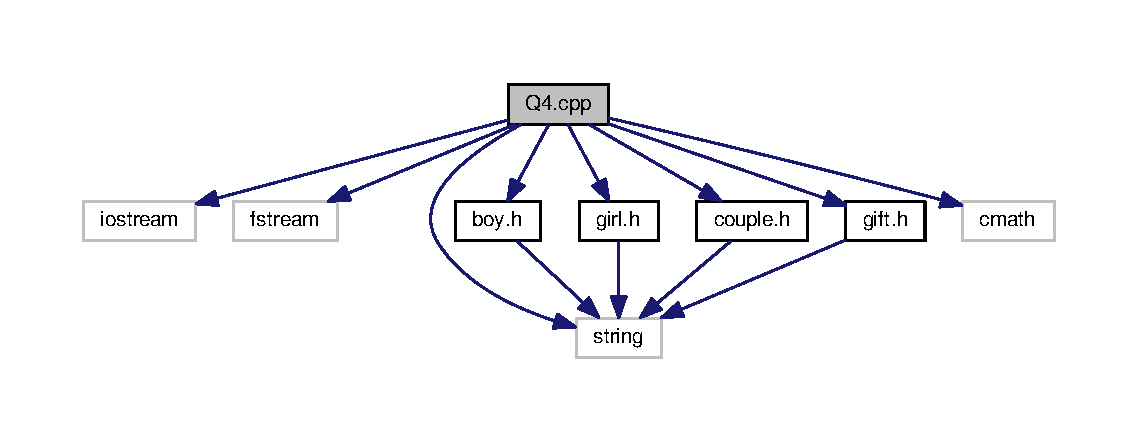
\includegraphics[width=350pt]{Q4_8cpp__incl}
\end{center}
\end{figure}
\subsection*{Functions}
\begin{DoxyCompactItemize}
\item 
void \hyperlink{Q4_8cpp_a5a408068bacb1c7add72673eb9d96bbc}{swap\+Couple} (\hyperlink{classcouple}{couple} \&a, \hyperlink{classcouple}{couple} \&b)
\item 
void \hyperlink{Q4_8cpp_ac5c65f5b5ec33f7b8ab8012de336fdb7}{swapC} (\hyperlink{classcouple}{couple} \&a, \hyperlink{classcouple}{couple} \&b)
\item 
int \hyperlink{Q4_8cpp_ae66f6b31b5ad750f1fe042a706a4e3d4}{main} ()
\end{DoxyCompactItemize}


\subsection{Function Documentation}
\index{Q4.\+cpp@{Q4.\+cpp}!main@{main}}
\index{main@{main}!Q4.\+cpp@{Q4.\+cpp}}
\subsubsection[{\texorpdfstring{main()}{main()}}]{\setlength{\rightskip}{0pt plus 5cm}int main (
\begin{DoxyParamCaption}
{}
\end{DoxyParamCaption}
)}\hypertarget{Q4_8cpp_ae66f6b31b5ad750f1fe042a706a4e3d4}{}\label{Q4_8cpp_ae66f6b31b5ad750f1fe042a706a4e3d4}
$<$ Read boys data

$<$ Read the gifts

$<$ Sort couples according to their happiness 
\begin{DoxyCode}
27 \{
28     ifstream boyPtr(\textcolor{stringliteral}{"boyrec.txt"}, ios::in);
29     ifstream girlPtr(\textcolor{stringliteral}{"girlrec.txt"}, ios::in);
30     ofstream opPtr(\textcolor{stringliteral}{"output.txt"}, ios::out);
31     ifstream giftPtr(\textcolor{stringliteral}{"gifts.txt"}, ios::in);
32     ofstream giftout(\textcolor{stringliteral}{"giftslog.txt"}, ios::out);
33     ofstream happiness(\textcolor{stringliteral}{"sortedHappiness.txt"}, ios::out);
34     ofstream compatibility(\textcolor{stringliteral}{"sortedComaptibility.txt"}, ios::out);
35     ofstream breakup(\textcolor{stringliteral}{"breakup.txt"}, ios::out);
36     ofstream newCouples(\textcolor{stringliteral}{"couples.txt"}, ios::out);
37 
38     \textcolor{keywordtype}{int} \hyperlink{lib7_8h_aeee5e31bf47987f4c471a1649ec9e43f}{noBoys} = 9,\hyperlink{lib7_8h_afbf77341ebcfec44fd5ed146e13668bf}{noGirls} = 6;
39     \hyperlink{classBoy}{Boy} boy[\hyperlink{lib7_8h_aeee5e31bf47987f4c471a1649ec9e43f}{noBoys}];
40     \hyperlink{classGirl}{Girl} girl[\hyperlink{lib7_8h_afbf77341ebcfec44fd5ed146e13668bf}{noGirls}];
41     \hyperlink{classcouple}{couple} \hyperlink{classcouple}{couple}[\hyperlink{lib7_8h_afbf77341ebcfec44fd5ed146e13668bf}{noGirls}];
42     \hyperlink{classGift}{Gift} gift[4*\hyperlink{lib7_8h_afbf77341ebcfec44fd5ed146e13668bf}{noGirls}];
43     \textcolor{keywordtype}{int} maint, budget,intelli,attr,i;
44     \textcolor{keywordtype}{string} name,girlName,boyName,type;
45     
47     \textcolor{keywordflow}{for}( i = 0; i < \hyperlink{lib7_8h_aeee5e31bf47987f4c471a1649ec9e43f}{noBoys}; i++) \{
48         boyPtr >> name >> type >>attr >> intelli >> budget ;
49         boy[i].\hyperlink{classBoy_aa6d16a472a01b4e7da0817fe94d9a2bd}{init}(name,type,attr,intelli,budget);
50     \}
51 
53     \textcolor{keywordflow}{for}( i = 0; i < \hyperlink{lib7_8h_afbf77341ebcfec44fd5ed146e13668bf}{noGirls}; i++) \{
54         girlPtr >> name >> type >> attr >> intelli >> maint ;
55         girl[i].\hyperlink{classGirl_aba849734c908a23bde2e5bd9c335c450}{init}(name,type,attr,intelli,budget);
56     \}
57 
59     \textcolor{keywordtype}{int} j = 0,k = 0;
60     \textcolor{keywordflow}{for}( i = 0; i < \hyperlink{lib7_8h_afbf77341ebcfec44fd5ed146e13668bf}{noGirls}; i++) \{
61         maint = girl[i].\hyperlink{classGirl_ac23543169a5e339a3c93fbd8aeb977ca}{getMaint}();
62         girlName = girl[i].\hyperlink{classGirl_a27a705fb94b92dfd6929d0bf4bcaf5e1}{getName}();
63         \textcolor{keywordflow}{for}( j = k; j < \hyperlink{lib7_8h_aeee5e31bf47987f4c471a1649ec9e43f}{noBoys}; j++) \{
64             budget = boy[j].\hyperlink{classBoy_a05c48b12091ebcad44ba86ba88514ac5}{getBudget}();
65             boyName = boy[j].\hyperlink{classBoy_acf59fd0074a6ea3413751a95b2970303}{getName}();
66             \textcolor{keywordflow}{if}(maint < budget && !(girl[i].getStatus() ) && !(boy[j].getStatus() ) ) \{
67                     opPtr << girlName << \textcolor{stringliteral}{"        "} << boyName << endl;
68                     couple[i].\hyperlink{classcouple_a3ee36a530603865ff58470bae84da220}{init}(boyName,boy[j].getType(), girlName,boy[j].getBudget(),girl[i].
      getMaint(),boy[j].getAttr(),girl[i].getAttr(),boy[j].getIntelli(),girl[i].getIntelli());
69                     girl[i].\hyperlink{classGirl_ac4e040efdf40d12044bda1b647e0d2da}{changeStatus}();
70                     boy[j].\hyperlink{classBoy_a2a8cc82d9332c07eb475198e46028d52}{changeStatus}();
71                     k++;
72                     \textcolor{keywordflow}{break};
73             \} \textcolor{keywordflow}{else} \{
74                 j--;
75             \}
76         \}
77     \}
78 
79     \textcolor{keywordtype}{int} val,pr;
80     std:: string ty;
82     \textcolor{keywordflow}{for}(i = 0; i < 2*\hyperlink{lib7_8h_afbf77341ebcfec44fd5ed146e13668bf}{noGirls}; i++) \{
83         giftPtr >> val >> pr >> ty;
84         gift[i].\hyperlink{classGift_aee7c5672f4d1ee738a7dbeb6f952fe1f}{init}(val,pr,ty);
85     \}
87     \textcolor{keywordtype}{int} currbud;
88     j = 0;
89     \textcolor{keywordflow}{for}(i = 0; i < \hyperlink{lib7_8h_afbf77341ebcfec44fd5ed146e13668bf}{noGirls}; i++) \{
90         currbud = couple[i].\hyperlink{classcouple_af4b090a72111d7ba566747e4e305a6ec}{getCurrBudget}() ;
91         \textcolor{keywordflow}{while}(currbud > gift[j].getPrice()) \{
92             pr = gift[j].\hyperlink{classGift_aa114ca9629b5f02e4df6731d33c69373}{getPrice}();
93             giftout << couple[i].\hyperlink{classcouple_afe07f86e775d20508e6cd139488af366}{getBoyname}() << \textcolor{stringliteral}{"  "} << couple[i].
      \hyperlink{classcouple_a7897320b780dbeaa85380c71803de9c2}{getGirlname}() << \textcolor{stringliteral}{"  "} <<  pr << endl;
94             couple[i].\hyperlink{classcouple_afa9889ca750dd53ffd06daf78cbee326}{changeCurrBudget}(pr);
95             j++;
96             currbud = couple[i].\hyperlink{classcouple_af4b090a72111d7ba566747e4e305a6ec}{getCurrBudget}() ;
97         \}
98     \}
99     \textcolor{comment}{/*}
100 \textcolor{comment}{    * Calculate Happiness of Girls
}
101 \textcolor{comment}{    */}
102     \textcolor{keywordtype}{int} bh,gh,cost;
103     \textcolor{keywordflow}{for}( i = 0; i< \hyperlink{lib7_8h_afbf77341ebcfec44fd5ed146e13668bf}{noGirls}; i++) \{
104         type = girl[i].\hyperlink{classGirl_a2b5bbd35287b7aa074f39702b564bc97}{getType}();
105         cost = couple[i].\hyperlink{classcouple_a5f31ac8019f5db29694dc36cdba958b8}{getCost}();
106         \textcolor{keywordflow}{if}(type == \textcolor{stringliteral}{"Choosy"}) \{
107             gh = log10(cost / girl[i].getMaint());
108         \} \textcolor{keywordflow}{else} \textcolor{keywordflow}{if}(type == \textcolor{stringliteral}{"Normal"}) \{
109             gh = cost / girl[i].\hyperlink{classGirl_ac23543169a5e339a3c93fbd8aeb977ca}{getMaint}();
110         \} \textcolor{keywordflow}{else} \textcolor{keywordflow}{if}(type == \textcolor{stringliteral}{"Desperate"}) \{
111             gh = exp(cost / girl[i].getMaint());
112         \}
113         couple[i].\hyperlink{classcouple_a526f48a752f261212d111a630f5730f4}{setGirlHappiness}(gh);
114     \}
115  
117     \textcolor{keywordflow}{for}(i = 0; i < \hyperlink{lib7_8h_afbf77341ebcfec44fd5ed146e13668bf}{noGirls}; i++) \{
118         type = couple[i].\hyperlink{classcouple_a687986a266cc984fa5d2114c888f52cf}{getBoyType}();
119         cost = couple[i].\hyperlink{classcouple_a5f31ac8019f5db29694dc36cdba958b8}{getCost}();
120         \textcolor{keywordflow}{if}(type == \textcolor{stringliteral}{"Miser"}) \{
121             bh = couple[i].\hyperlink{classcouple_a92496b42f9d1392013c4d7456318ad70}{getBudget}() - cost;
122         \} \textcolor{keywordflow}{else} \textcolor{keywordflow}{if}(type == \textcolor{stringliteral}{"Generous"}) \{
123             bh = couple[i].\hyperlink{classcouple_ada2f9b79cede186a0e9bcd6b48bec804}{getGirlHappiness}();
124         \} \textcolor{keywordflow}{else} \{
125             bh = girl[i].\hyperlink{classGirl_afe73c4c4f180aa8f5e0bc4f87455ec0b}{getIntelligence}();
126         \}
127         couple[i].\hyperlink{classcouple_a50a890cb7ffd3a44f0201b8e0d84f744}{setBoyHappiness}(bh);
128         couple[i].\hyperlink{classcouple_aaaadc39a9f265907581925ef579c7214}{setHappiness}();
129     \}
130 
131     \textcolor{keywordtype}{int} h1,h2;
132 
133     k = 3;
135     \textcolor{keywordflow}{for}(i = 0; i < \hyperlink{lib7_8h_afbf77341ebcfec44fd5ed146e13668bf}{noGirls}; i++) \{
136         h1 = couple[i].\hyperlink{classcouple_a31d0a1c8acff06a64ebc2e2f6d9a68b1}{getHappiness}();
137         \textcolor{keywordflow}{for}(j = i+1; j < \hyperlink{lib7_8h_afbf77341ebcfec44fd5ed146e13668bf}{noGirls}; j++) \{
138             h2 = couple[j].\hyperlink{classcouple_a31d0a1c8acff06a64ebc2e2f6d9a68b1}{getHappiness}();
139             \textcolor{keywordflow}{if}(h1 > h2) \{
140                 \hyperlink{Q4_8cpp_a5a408068bacb1c7add72673eb9d96bbc}{swapCouple}(couple[i], couple[j]);
141             \}
142         \}
143     \}
144 
146     \textcolor{keywordflow}{for}(i = 0; i< k; i++) \{
147         happiness << couple[i].\hyperlink{classcouple_afe07f86e775d20508e6cd139488af366}{getBoyname}() << \textcolor{stringliteral}{"  "} << couple[i].
      \hyperlink{classcouple_a7897320b780dbeaa85380c71803de9c2}{getGirlname}() << endl;
148     \}
149 
151     \textcolor{keywordflow}{for}( i = 0; i < \hyperlink{lib7_8h_afbf77341ebcfec44fd5ed146e13668bf}{noGirls}; i++) \{
152         couple[i].\hyperlink{classcouple_a91bc77488fe8b5d30643b9ff0a56d359}{setCompatibility}();
153     \}
154 
156     \textcolor{keywordflow}{for}(i = 0; i < \hyperlink{lib7_8h_afbf77341ebcfec44fd5ed146e13668bf}{noGirls}; i++) \{
157         h1 = couple[i].\hyperlink{classcouple_a43d2852ce692307280ba9ab2366c16eb}{getCompatibility}();
158         \textcolor{keywordflow}{for}(j = i+1; j < \hyperlink{lib7_8h_afbf77341ebcfec44fd5ed146e13668bf}{noGirls}; j++) \{
159             h2 = couple[j].\hyperlink{classcouple_a43d2852ce692307280ba9ab2366c16eb}{getCompatibility}();
160             \textcolor{keywordflow}{if}(h1 > h2) \{
161                 \hyperlink{Q4_8cpp_ac5c65f5b5ec33f7b8ab8012de336fdb7}{swapC}(couple[i],couple[j]);
162             \}
163         \}
164     \}
165 
167     k = 0;
168     \textcolor{keywordtype}{int} ind[100],p = 2;
169     \textcolor{keywordflow}{for}(i = noGirls - k; i < \hyperlink{lib7_8h_afbf77341ebcfec44fd5ed146e13668bf}{noGirls}; i++) \{
170         breakup << couple[i].\hyperlink{classcouple_afe07f86e775d20508e6cd139488af366}{getBoyname}() << \textcolor{stringliteral}{"  "} << couple[i].
      \hyperlink{classcouple_a7897320b780dbeaa85380c71803de9c2}{getGirlname}() << endl;
171         ind[i] = 100;
172     \}
173 
175     \textcolor{keywordflow}{for}( i = noGirls - p; i < \hyperlink{lib7_8h_afbf77341ebcfec44fd5ed146e13668bf}{noGirls}; i++) \{
176         maint = girl[i].\hyperlink{classGirl_ac23543169a5e339a3c93fbd8aeb977ca}{getMaint}();
177         girlName = girl[i].\hyperlink{classGirl_a27a705fb94b92dfd6929d0bf4bcaf5e1}{getName}();
178         \textcolor{keywordflow}{for}( j = k; j < \hyperlink{lib7_8h_aeee5e31bf47987f4c471a1649ec9e43f}{noBoys}; j++) \{
179             budget = boy[j].\hyperlink{classBoy_a05c48b12091ebcad44ba86ba88514ac5}{getBudget}();
180             boyName = boy[j].\hyperlink{classBoy_acf59fd0074a6ea3413751a95b2970303}{getName}();
181             \textcolor{keywordflow}{if}(maint < budget && !(boy[j].getStatus() ) ) \{
182                     newCouples << girlName << \textcolor{stringliteral}{"        "} << boyName << endl;
183                     couple[i].\hyperlink{classcouple_a3ee36a530603865ff58470bae84da220}{init}(boyName,boy[j].getType(), girlName,boy[j].getBudget(),girl[i].
      getMaint(),boy[j].getAttr(),girl[i].getAttr(),boy[j].getIntelli(),girl[i].getIntelli());
184                     girl[i].\hyperlink{classGirl_ac4e040efdf40d12044bda1b647e0d2da}{changeStatus}();
185                     boy[j].\hyperlink{classBoy_a2a8cc82d9332c07eb475198e46028d52}{changeStatus}();
186                     k++;
187                     \textcolor{keywordflow}{break};
188             \} 
189         \}
190     \}
191 
193     \textcolor{keywordflow}{for}(i = 0; i < \hyperlink{lib7_8h_aeee5e31bf47987f4c471a1649ec9e43f}{noBoys}; i++) \{
194         \textcolor{keywordflow}{if}(ind[i] == 100) \{
195             boy[i].\hyperlink{classBoy_a2a8cc82d9332c07eb475198e46028d52}{changeStatus}();
196         \}
197     \}
198 
199 \}
\end{DoxyCode}
\index{Q4.\+cpp@{Q4.\+cpp}!swapC@{swapC}}
\index{swapC@{swapC}!Q4.\+cpp@{Q4.\+cpp}}
\subsubsection[{\texorpdfstring{swap\+C(couple \&a, couple \&b)}{swapC(couple &a, couple &b)}}]{\setlength{\rightskip}{0pt plus 5cm}void swapC (
\begin{DoxyParamCaption}
\item[{{\bf couple} \&}]{a, }
\item[{{\bf couple} \&}]{b}
\end{DoxyParamCaption}
)}\hypertarget{Q4_8cpp_ac5c65f5b5ec33f7b8ab8012de336fdb7}{}\label{Q4_8cpp_ac5c65f5b5ec33f7b8ab8012de336fdb7}

\begin{DoxyCode}
20 \{
21     \hyperlink{classcouple}{couple} temp = a;
22     a = b;
23     b = temp;
24 \}
\end{DoxyCode}
\index{Q4.\+cpp@{Q4.\+cpp}!swap\+Couple@{swap\+Couple}}
\index{swap\+Couple@{swap\+Couple}!Q4.\+cpp@{Q4.\+cpp}}
\subsubsection[{\texorpdfstring{swap\+Couple(couple \&a, couple \&b)}{swapCouple(couple &a, couple &b)}}]{\setlength{\rightskip}{0pt plus 5cm}void swap\+Couple (
\begin{DoxyParamCaption}
\item[{{\bf couple} \&}]{a, }
\item[{{\bf couple} \&}]{b}
\end{DoxyParamCaption}
)}\hypertarget{Q4_8cpp_a5a408068bacb1c7add72673eb9d96bbc}{}\label{Q4_8cpp_a5a408068bacb1c7add72673eb9d96bbc}

\begin{DoxyCode}
13 \{
14     \hyperlink{classcouple}{couple} temp = a;
15     a = b;
16     b = temp;
17 \}
\end{DoxyCode}

\hypertarget{Q5_8cpp}{}\section{Q5.\+cpp File Reference}
\label{Q5_8cpp}\index{Q5.\+cpp@{Q5.\+cpp}}
{\ttfamily \#include $<$iostream$>$}\\*
{\ttfamily \#include $<$fstream$>$}\\*
{\ttfamily \#include $<$string$>$}\\*
{\ttfamily \#include \char`\"{}boy.\+h\char`\"{}}\\*
{\ttfamily \#include \char`\"{}girl.\+h\char`\"{}}\\*
{\ttfamily \#include \char`\"{}couple.\+h\char`\"{}}\\*
{\ttfamily \#include \char`\"{}gift.\+h\char`\"{}}\\*
{\ttfamily \#include $<$cmath$>$}\\*
Include dependency graph for Q5.\+cpp\+:
\nopagebreak
\begin{figure}[H]
\begin{center}
\leavevmode
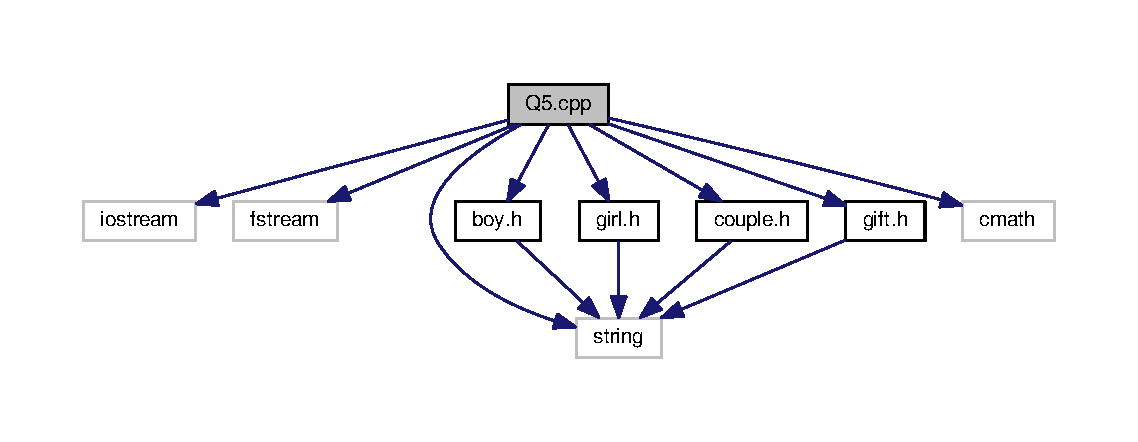
\includegraphics[width=350pt]{Q5_8cpp__incl}
\end{center}
\end{figure}
\subsection*{Functions}
\begin{DoxyCompactItemize}
\item 
void \hyperlink{Q5_8cpp_afe82d5f9e60375f604b0e204e6110d70}{swap\+Boys} (\hyperlink{classBoy}{Boy} \&a, \hyperlink{classBoy}{Boy} \&b)
\item 
void \hyperlink{Q5_8cpp_a19020e77c0c6aa7d46b702d74abb6a89}{swap\+Girls} (\hyperlink{classGirl}{Girl} \&a, \hyperlink{classGirl}{Girl} \&b)
\item 
void \hyperlink{Q5_8cpp_a5a408068bacb1c7add72673eb9d96bbc}{swap\+Couple} (\hyperlink{classcouple}{couple} \&a, \hyperlink{classcouple}{couple} \&b)
\item 
void \hyperlink{Q5_8cpp_ac5c65f5b5ec33f7b8ab8012de336fdb7}{swapC} (\hyperlink{classcouple}{couple} \&a, \hyperlink{classcouple}{couple} \&b)
\item 
int \hyperlink{Q5_8cpp_ae66f6b31b5ad750f1fe042a706a4e3d4}{main} ()
\end{DoxyCompactItemize}


\subsection{Function Documentation}
\index{Q5.\+cpp@{Q5.\+cpp}!main@{main}}
\index{main@{main}!Q5.\+cpp@{Q5.\+cpp}}
\subsubsection[{\texorpdfstring{main()}{main()}}]{\setlength{\rightskip}{0pt plus 5cm}int main (
\begin{DoxyParamCaption}
{}
\end{DoxyParamCaption}
)}\hypertarget{Q5_8cpp_ae66f6b31b5ad750f1fe042a706a4e3d4}{}\label{Q5_8cpp_ae66f6b31b5ad750f1fe042a706a4e3d4}
$<$ Read boys data

$<$ Read the gifts 
\begin{DoxyCode}
41 \{
42     ifstream boyPtr(\textcolor{stringliteral}{"boyrec.txt"}, ios::in);
43     ifstream girlPtr(\textcolor{stringliteral}{"girlrec.txt"}, ios::in);
44     ofstream opPtr(\textcolor{stringliteral}{"output.txt"}, ios::out);
45     ifstream giftPtr(\textcolor{stringliteral}{"gifts.txt"}, ios::in);
46     ofstream giftout(\textcolor{stringliteral}{"giftslog.txt"}, ios::out);
47     ofstream happiness(\textcolor{stringliteral}{"sortedHappiness.txt"}, ios::out);
48     ofstream compatibility(\textcolor{stringliteral}{"sortedComaptibility.txt"}, ios::out);
49     ofstream breakup(\textcolor{stringliteral}{"breakup.txt"}, ios::out);
50     ofstream newCouples(\textcolor{stringliteral}{"couples.txt"}, ios::out);
51 
52     \textcolor{keywordtype}{int} \hyperlink{lib7_8h_aeee5e31bf47987f4c471a1649ec9e43f}{noBoys} = 9,\hyperlink{lib7_8h_afbf77341ebcfec44fd5ed146e13668bf}{noGirls} = 6,max,ind,j;
53     \hyperlink{classBoy}{Boy} boy[\hyperlink{lib7_8h_aeee5e31bf47987f4c471a1649ec9e43f}{noBoys}];
54     \hyperlink{classGirl}{Girl} girl[\hyperlink{lib7_8h_afbf77341ebcfec44fd5ed146e13668bf}{noGirls}];
55     \hyperlink{classcouple}{couple} \hyperlink{classcouple}{couple}[\hyperlink{lib7_8h_afbf77341ebcfec44fd5ed146e13668bf}{noGirls}];
56     \hyperlink{classGift}{Gift} gift[4*\hyperlink{lib7_8h_afbf77341ebcfec44fd5ed146e13668bf}{noGirls}];
57     \textcolor{keywordtype}{int} maint, budget,intelli,attr,i;
58     \textcolor{keywordtype}{string} name,girlName,boyName,type;
59     
61     \textcolor{keywordflow}{for}( i = 0; i < \hyperlink{lib7_8h_aeee5e31bf47987f4c471a1649ec9e43f}{noBoys}; i++) \{
62         boyPtr >> name >> type >>attr >> intelli >> budget ;
63         boy[i].\hyperlink{classBoy_aa6d16a472a01b4e7da0817fe94d9a2bd}{init}(name,type,attr,intelli,budget);
64     \}
65 
67     \textcolor{keywordflow}{for}( i = 0; i < \hyperlink{lib7_8h_afbf77341ebcfec44fd5ed146e13668bf}{noGirls}; i++) \{
68         girlPtr >> name >> type >> attr >> intelli >> maint ;
69         girl[i].\hyperlink{classGirl_aba849734c908a23bde2e5bd9c335c450}{init}(name,type,attr,intelli,budget);
70     \}
71 
72     \textcolor{keywordtype}{int} val,pr;
73     std:: string ty;
75     \textcolor{keywordflow}{for}(i = 0; i < 4*\hyperlink{lib7_8h_afbf77341ebcfec44fd5ed146e13668bf}{noGirls}; i++) \{
76         giftPtr >> val >> pr >> ty;
77         gift[i].\hyperlink{classGift_aee7c5672f4d1ee738a7dbeb6f952fe1f}{init}(val,pr,ty);
78     \}
79     
81     \textcolor{keywordflow}{for}( i = 0; i< \hyperlink{lib7_8h_aeee5e31bf47987f4c471a1649ec9e43f}{noBoys}; i++) \{
82         \textcolor{keywordflow}{for}( j = 0; j < \hyperlink{lib7_8h_aeee5e31bf47987f4c471a1649ec9e43f}{noBoys}; j++) \{
83             \textcolor{keywordflow}{if}( boy[i].getAttr() > boy[j].getAttr()) \{
84                 \hyperlink{Q5_8cpp_afe82d5f9e60375f604b0e204e6110d70}{swapBoys}(boy[i],boy[j]);
85             \}
86         \}
87     \}
88 
90     \textcolor{keywordflow}{for}( i = 0; i< \hyperlink{lib7_8h_afbf77341ebcfec44fd5ed146e13668bf}{noGirls}; i++) \{
91         \textcolor{keywordflow}{for}( j = 0; j < \hyperlink{lib7_8h_afbf77341ebcfec44fd5ed146e13668bf}{noGirls}; j++) \{
92             \textcolor{keywordflow}{if}( girl[i].getMaint() > girl[j].getMaint()) \{
93                 \hyperlink{Q5_8cpp_a19020e77c0c6aa7d46b702d74abb6a89}{swapGirls}(girl[i],girl[j]);
94             \}
95         \}
96     \}
97 
98     \textcolor{keywordtype}{int} p;
99     \textcolor{keywordflow}{for}(i = 0; i < \hyperlink{lib7_8h_afbf77341ebcfec44fd5ed146e13668bf}{noGirls}; i++) \{
100         \textcolor{keywordflow}{if}( (i % 2) == 0) \{
101             p = i;
102             \textcolor{keywordflow}{while}( girl[p].getStatus() && p < noGirls) \{
103                 p++;
104             \}
105 
106             \textcolor{keywordflow}{if}( p == noGirls) \textcolor{keywordflow}{break};
107             max = 0;
108             \textcolor{keywordflow}{for}(j = 0; j < \hyperlink{lib7_8h_aeee5e31bf47987f4c471a1649ec9e43f}{noBoys}; j++) \{
109                 \textcolor{keywordflow}{if}( !(boy[j].getStatus()) && boy[j].getBudget() > max) \{
110                     max = boy[j].\hyperlink{classBoy_a05c48b12091ebcad44ba86ba88514ac5}{getBudget}();
111                     ind = j;
112                 \}
113             \}
114 
115             couple[i].\hyperlink{classcouple_a3ee36a530603865ff58470bae84da220}{init}(boy[ind].getName(),boy[ind].getType(), girl[p].getName(),boy[ind].getBudget(
      ),girl[p].getMaint(),boy[ind].getAttr(),girl[p].getAttr(),boy[ind].getIntelli(),girl[p].getIntelli());
116             girl[p].\hyperlink{classGirl_ac4e040efdf40d12044bda1b647e0d2da}{changeStatus}();
117             boy[ind].\hyperlink{classBoy_a2a8cc82d9332c07eb475198e46028d52}{changeStatus}();
118         \} \textcolor{keywordflow}{else} \{
119             p = i;
120             \textcolor{keywordflow}{while}( boy[p].getStatus() && p < noBoys) \{
121                 p++;
122             \}
123             max = 0;
124             \textcolor{keywordflow}{for}(j = 0; j < \hyperlink{lib7_8h_afbf77341ebcfec44fd5ed146e13668bf}{noGirls}; j++)\{
125                 \textcolor{keywordflow}{if}( !(girl[j].getStatus()) && girl[j].getAttr() > max) \{
126                     max = girl[j].\hyperlink{classGirl_aa86bcd99f1fbcd2359a12b9a94e32486}{getAttr}();
127                     ind = j;
128                 \}
129             \}
130 
131             couple[i].\hyperlink{classcouple_a3ee36a530603865ff58470bae84da220}{init}(boy[p].getName(),boy[p].getType(), girl[ind].getName(),boy[p].getBudget(),
      girl[ind].getMaint(),boy[p].getAttr(),girl[ind].getAttr(),boy[p].getIntelli(),girl[ind].getIntelli());
132             girl[ind].\hyperlink{classGirl_ac4e040efdf40d12044bda1b647e0d2da}{changeStatus}();
133             boy[p].\hyperlink{classBoy_a2a8cc82d9332c07eb475198e46028d52}{changeStatus}();
134         \}
135     \}
136 
137     \textcolor{keywordflow}{for}(i = 0; i < \hyperlink{lib7_8h_afbf77341ebcfec44fd5ed146e13668bf}{noGirls}; i++) \{
138         newCouples << couple[i].\hyperlink{classcouple_afe07f86e775d20508e6cd139488af366}{getBoyname}() << \textcolor{stringliteral}{"   "} << couple[i].
      \hyperlink{classcouple_a7897320b780dbeaa85380c71803de9c2}{getGirlname}() << endl;
139     \}
140 \}
\end{DoxyCode}
\index{Q5.\+cpp@{Q5.\+cpp}!swap\+Boys@{swap\+Boys}}
\index{swap\+Boys@{swap\+Boys}!Q5.\+cpp@{Q5.\+cpp}}
\subsubsection[{\texorpdfstring{swap\+Boys(\+Boy \&a, Boy \&b)}{swapBoys(Boy &a, Boy &b)}}]{\setlength{\rightskip}{0pt plus 5cm}void swap\+Boys (
\begin{DoxyParamCaption}
\item[{{\bf Boy} \&}]{a, }
\item[{{\bf Boy} \&}]{b}
\end{DoxyParamCaption}
)}\hypertarget{Q5_8cpp_afe82d5f9e60375f604b0e204e6110d70}{}\label{Q5_8cpp_afe82d5f9e60375f604b0e204e6110d70}

\begin{DoxyCode}
13 \{
14     \hyperlink{classBoy}{Boy} temp = a;
15     a = b;
16     b = temp;
17 \}
\end{DoxyCode}
\index{Q5.\+cpp@{Q5.\+cpp}!swapC@{swapC}}
\index{swapC@{swapC}!Q5.\+cpp@{Q5.\+cpp}}
\subsubsection[{\texorpdfstring{swap\+C(couple \&a, couple \&b)}{swapC(couple &a, couple &b)}}]{\setlength{\rightskip}{0pt plus 5cm}void swapC (
\begin{DoxyParamCaption}
\item[{{\bf couple} \&}]{a, }
\item[{{\bf couple} \&}]{b}
\end{DoxyParamCaption}
)}\hypertarget{Q5_8cpp_ac5c65f5b5ec33f7b8ab8012de336fdb7}{}\label{Q5_8cpp_ac5c65f5b5ec33f7b8ab8012de336fdb7}

\begin{DoxyCode}
34 \{
35     \hyperlink{classcouple}{couple} temp = a;
36     a = b;
37     b = temp;
38 \}
\end{DoxyCode}
\index{Q5.\+cpp@{Q5.\+cpp}!swap\+Couple@{swap\+Couple}}
\index{swap\+Couple@{swap\+Couple}!Q5.\+cpp@{Q5.\+cpp}}
\subsubsection[{\texorpdfstring{swap\+Couple(couple \&a, couple \&b)}{swapCouple(couple &a, couple &b)}}]{\setlength{\rightskip}{0pt plus 5cm}void swap\+Couple (
\begin{DoxyParamCaption}
\item[{{\bf couple} \&}]{a, }
\item[{{\bf couple} \&}]{b}
\end{DoxyParamCaption}
)}\hypertarget{Q5_8cpp_a5a408068bacb1c7add72673eb9d96bbc}{}\label{Q5_8cpp_a5a408068bacb1c7add72673eb9d96bbc}

\begin{DoxyCode}
27 \{
28     \hyperlink{classcouple}{couple} temp = a;
29     a = b;
30     b = temp;
31 \}
\end{DoxyCode}
\index{Q5.\+cpp@{Q5.\+cpp}!swap\+Girls@{swap\+Girls}}
\index{swap\+Girls@{swap\+Girls}!Q5.\+cpp@{Q5.\+cpp}}
\subsubsection[{\texorpdfstring{swap\+Girls(\+Girl \&a, Girl \&b)}{swapGirls(Girl &a, Girl &b)}}]{\setlength{\rightskip}{0pt plus 5cm}void swap\+Girls (
\begin{DoxyParamCaption}
\item[{{\bf Girl} \&}]{a, }
\item[{{\bf Girl} \&}]{b}
\end{DoxyParamCaption}
)}\hypertarget{Q5_8cpp_a19020e77c0c6aa7d46b702d74abb6a89}{}\label{Q5_8cpp_a19020e77c0c6aa7d46b702d74abb6a89}

\begin{DoxyCode}
20 \{
21     \hyperlink{classGirl}{Girl} temp = a;
22     a = b;
23     b = temp;
24 \}
\end{DoxyCode}

\hypertarget{Q6_8cpp}{}\section{Q6.\+cpp File Reference}
\label{Q6_8cpp}\index{Q6.\+cpp@{Q6.\+cpp}}
{\ttfamily \#include $<$iostream$>$}\\*
{\ttfamily \#include $<$fstream$>$}\\*
{\ttfamily \#include $<$string$>$}\\*
{\ttfamily \#include \char`\"{}boy.\+h\char`\"{}}\\*
{\ttfamily \#include \char`\"{}girl.\+h\char`\"{}}\\*
{\ttfamily \#include \char`\"{}couple.\+h\char`\"{}}\\*
{\ttfamily \#include \char`\"{}gift.\+h\char`\"{}}\\*
{\ttfamily \#include $<$cmath$>$}\\*
Include dependency graph for Q6.\+cpp\+:
\nopagebreak
\begin{figure}[H]
\begin{center}
\leavevmode
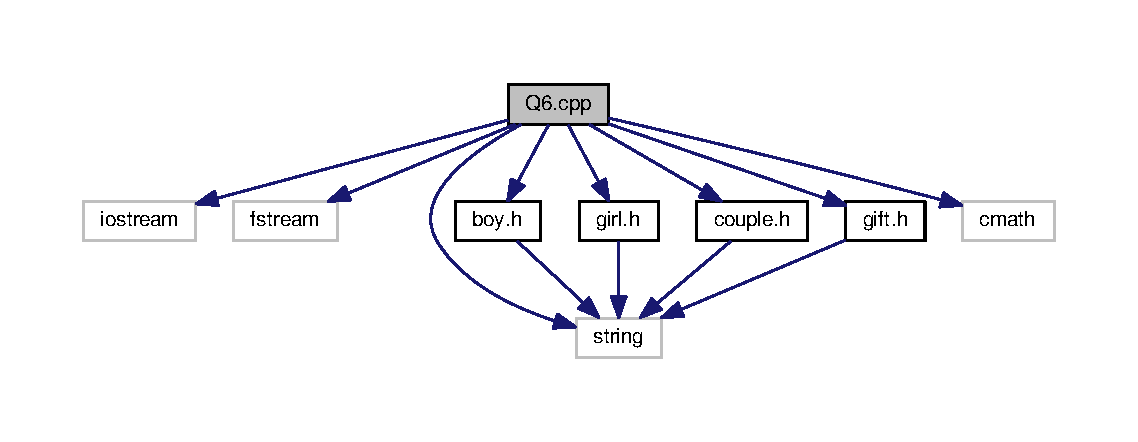
\includegraphics[width=350pt]{Q6_8cpp__incl}
\end{center}
\end{figure}
\subsection*{Macros}
\begin{DoxyCompactItemize}
\item 
\#define \hyperlink{Q6_8cpp_a0acb682b8260ab1c60b918599864e2e5}{T}~5
\end{DoxyCompactItemize}
\subsection*{Functions}
\begin{DoxyCompactItemize}
\item 
void \hyperlink{Q6_8cpp_a5a408068bacb1c7add72673eb9d96bbc}{swap\+Couple} (\hyperlink{classcouple}{couple} \&a, \hyperlink{classcouple}{couple} \&b)
\item 
void \hyperlink{Q6_8cpp_ac5c65f5b5ec33f7b8ab8012de336fdb7}{swapC} (\hyperlink{classcouple}{couple} \&a, \hyperlink{classcouple}{couple} \&b)
\item 
int \hyperlink{Q6_8cpp_ae66f6b31b5ad750f1fe042a706a4e3d4}{main} ()
\end{DoxyCompactItemize}


\subsection{Macro Definition Documentation}
\index{Q6.\+cpp@{Q6.\+cpp}!T@{T}}
\index{T@{T}!Q6.\+cpp@{Q6.\+cpp}}
\subsubsection[{\texorpdfstring{T}{T}}]{\setlength{\rightskip}{0pt plus 5cm}\#define T~5}\hypertarget{Q6_8cpp_a0acb682b8260ab1c60b918599864e2e5}{}\label{Q6_8cpp_a0acb682b8260ab1c60b918599864e2e5}


\subsection{Function Documentation}
\index{Q6.\+cpp@{Q6.\+cpp}!main@{main}}
\index{main@{main}!Q6.\+cpp@{Q6.\+cpp}}
\subsubsection[{\texorpdfstring{main()}{main()}}]{\setlength{\rightskip}{0pt plus 5cm}int main (
\begin{DoxyParamCaption}
{}
\end{DoxyParamCaption}
)}\hypertarget{Q6_8cpp_ae66f6b31b5ad750f1fe042a706a4e3d4}{}\label{Q6_8cpp_ae66f6b31b5ad750f1fe042a706a4e3d4}
$<$ Read boys data

$<$ Read the gifts

$<$ Allocate Gifts

$<$ Sort couples according to their happiness

$<$ Make Couples 
\begin{DoxyCode}
29 \{
30     ifstream boyPtr(\textcolor{stringliteral}{"boyrec.txt"}, ios::in);
31     ifstream girlPtr(\textcolor{stringliteral}{"girlrec.txt"}, ios::in);
32     ofstream opPtr(\textcolor{stringliteral}{"output.txt"}, ios::out);
33     ifstream giftPtr(\textcolor{stringliteral}{"gifts.txt"}, ios::in);
34     ofstream giftout(\textcolor{stringliteral}{"giftslog.txt"}, ios::out);
35     ofstream newCouples(\textcolor{stringliteral}{"couples.txt"}, ios::out);
36 
37     \textcolor{keywordtype}{int} \hyperlink{lib7_8h_aeee5e31bf47987f4c471a1649ec9e43f}{noBoys} = 9,\hyperlink{lib7_8h_afbf77341ebcfec44fd5ed146e13668bf}{noGirls} = 6;
38     \hyperlink{classBoy}{Boy} boy[\hyperlink{lib7_8h_aeee5e31bf47987f4c471a1649ec9e43f}{noBoys}];
39     \hyperlink{classGirl}{Girl} girl[\hyperlink{lib7_8h_afbf77341ebcfec44fd5ed146e13668bf}{noGirls}];
40     \hyperlink{classcouple}{couple} \hyperlink{classcouple}{couple}[\hyperlink{lib7_8h_afbf77341ebcfec44fd5ed146e13668bf}{noGirls}];
41     \hyperlink{classGift}{Gift} gift[4*\hyperlink{lib7_8h_afbf77341ebcfec44fd5ed146e13668bf}{noGirls}];
42     \textcolor{keywordtype}{int} maint, budget,intelli,attr,i;
43     \textcolor{keywordtype}{string} name,girlName,boyName,type;
44     
46     \textcolor{keywordflow}{for}( i = 0; i < \hyperlink{lib7_8h_aeee5e31bf47987f4c471a1649ec9e43f}{noBoys}; i++) \{
47         boyPtr >> name >> type >>attr >> intelli >> budget ;
48         boy[i].\hyperlink{classBoy_aa6d16a472a01b4e7da0817fe94d9a2bd}{init}(name,type,attr,intelli,budget);
49     \}
50 
52     \textcolor{keywordflow}{for}( i = 0; i < \hyperlink{lib7_8h_afbf77341ebcfec44fd5ed146e13668bf}{noGirls}; i++) \{
53         girlPtr >> name >> type >> attr >> intelli >> maint ;
54         girl[i].\hyperlink{classGirl_aba849734c908a23bde2e5bd9c335c450}{init}(name,type,attr,intelli,budget);
55     \}
56 
57     \textcolor{keywordtype}{int} val,pr;
58     std:: string ty;
60     \textcolor{keywordflow}{for}(i = 0; i < 14; i++) \{
61         giftPtr >> val >> pr >> ty;
62         gift[i].\hyperlink{classGift_aee7c5672f4d1ee738a7dbeb6f952fe1f}{init}(val,pr,ty);
63     \}
64 
66     \textcolor{keywordtype}{int} j = 0,k = 0,ind = 0;
67     \textcolor{keywordflow}{for}( i = 0; i < \hyperlink{lib7_8h_afbf77341ebcfec44fd5ed146e13668bf}{noGirls}; i++) \{
68         maint = girl[i].\hyperlink{classGirl_ac23543169a5e339a3c93fbd8aeb977ca}{getMaint}();
69         girlName = girl[i].\hyperlink{classGirl_a27a705fb94b92dfd6929d0bf4bcaf5e1}{getName}();
70         \textcolor{keywordflow}{for}( j = k; j < \hyperlink{lib7_8h_aeee5e31bf47987f4c471a1649ec9e43f}{noBoys}; j++) \{
71             budget = boy[j].\hyperlink{classBoy_a05c48b12091ebcad44ba86ba88514ac5}{getBudget}();
72             boyName = boy[j].\hyperlink{classBoy_acf59fd0074a6ea3413751a95b2970303}{getName}();
73             \textcolor{keywordflow}{if}(maint < budget && !(girl[i].getStatus() ) && !(boy[j].getStatus() ) ) \{
74                     opPtr << girlName << \textcolor{stringliteral}{"        "} << boyName << endl;
75                     couple[i].\hyperlink{classcouple_a3ee36a530603865ff58470bae84da220}{init}(boyName,boy[j].getType(), girlName,boy[j].getBudget(),girl[i].
      getMaint(),boy[j].getAttr(),girl[i].getAttr(),boy[j].getIntelli(),girl[i].getIntelli());
76                     girl[i].\hyperlink{classGirl_ac4e040efdf40d12044bda1b647e0d2da}{changeStatus}();
77                     boy[j].\hyperlink{classBoy_a2a8cc82d9332c07eb475198e46028d52}{changeStatus}();
78                     k++;
79                     \textcolor{keywordflow}{break};
80             \} \textcolor{keywordflow}{else} \{
81                 j--;
82             \}
83         \}
84     \}
85 
86     \textcolor{keywordtype}{int} counter;
87     \textcolor{keywordflow}{for}( counter = 0; counter < \hyperlink{Q6_8cpp_a0acb682b8260ab1c60b918599864e2e5}{T}; counter++) \{
89         \textcolor{keywordtype}{int} currbud;
90         j = 0;
91         \textcolor{keywordflow}{for}(i = 0; i < \hyperlink{lib7_8h_afbf77341ebcfec44fd5ed146e13668bf}{noGirls}; i++) \{
92             currbud = couple[i].\hyperlink{classcouple_af4b090a72111d7ba566747e4e305a6ec}{getCurrBudget}() ;
93             \textcolor{keywordflow}{while}(currbud > gift[j].getPrice() && j < 14) \{
94                 pr = gift[j].\hyperlink{classGift_aa114ca9629b5f02e4df6731d33c69373}{getPrice}();
95                 giftout << couple[i].\hyperlink{classcouple_afe07f86e775d20508e6cd139488af366}{getBoyname}() << \textcolor{stringliteral}{"  "} << couple[i].
      \hyperlink{classcouple_a7897320b780dbeaa85380c71803de9c2}{getGirlname}() << \textcolor{stringliteral}{"  "} <<  pr << endl;
96                 couple[i].\hyperlink{classcouple_afa9889ca750dd53ffd06daf78cbee326}{changeCurrBudget}(pr);
97                 j++;
98                 currbud = couple[i].\hyperlink{classcouple_af4b090a72111d7ba566747e4e305a6ec}{getCurrBudget}() ;
99             \}
100         \}
101 
102             \textcolor{comment}{/*}
103 \textcolor{comment}{        * Calculate Happiness of Girls}
104 \textcolor{comment}{        */}
105         \textcolor{keywordtype}{int} bh,gh,cost;
106         \textcolor{keywordflow}{for}( i = 0; i< \hyperlink{lib7_8h_afbf77341ebcfec44fd5ed146e13668bf}{noGirls}; i++) \{
107             type = girl[i].\hyperlink{classGirl_a2b5bbd35287b7aa074f39702b564bc97}{getType}();
108             cost = couple[i].\hyperlink{classcouple_a5f31ac8019f5db29694dc36cdba958b8}{getCost}();
109             \textcolor{keywordflow}{if}(type == \textcolor{stringliteral}{"Choosy"}) \{
110                 gh = log10(cost / girl[i].getMaint());
111             \} \textcolor{keywordflow}{else} \textcolor{keywordflow}{if}(type == \textcolor{stringliteral}{"Normal"}) \{
112                 gh = cost / girl[i].\hyperlink{classGirl_ac23543169a5e339a3c93fbd8aeb977ca}{getMaint}();
113             \} \textcolor{keywordflow}{else} \textcolor{keywordflow}{if}(type == \textcolor{stringliteral}{"Desperate"}) \{
114                 gh = exp(cost / girl[i].getMaint());
115             \}
116             couple[i].\hyperlink{classcouple_a526f48a752f261212d111a630f5730f4}{setGirlHappiness}(gh);
117         \}
118 
120         \textcolor{keywordflow}{for}(i = 0; i < \hyperlink{lib7_8h_afbf77341ebcfec44fd5ed146e13668bf}{noGirls}; i++) \{
121             type = couple[i].\hyperlink{classcouple_a687986a266cc984fa5d2114c888f52cf}{getBoyType}();
122             cost = couple[i].\hyperlink{classcouple_a5f31ac8019f5db29694dc36cdba958b8}{getCost}();
123             \textcolor{keywordflow}{if}(type == \textcolor{stringliteral}{"Miser"}) \{
124                 bh = couple[i].\hyperlink{classcouple_a92496b42f9d1392013c4d7456318ad70}{getBudget}() - cost;
125             \} \textcolor{keywordflow}{else} \textcolor{keywordflow}{if}(type == \textcolor{stringliteral}{"Generous"}) \{
126                 bh = couple[i].\hyperlink{classcouple_ada2f9b79cede186a0e9bcd6b48bec804}{getGirlHappiness}();
127             \} \textcolor{keywordflow}{else} \{
128                 bh = girl[i].\hyperlink{classGirl_afe73c4c4f180aa8f5e0bc4f87455ec0b}{getIntelligence}();
129             \}
130             couple[i].\hyperlink{classcouple_a50a890cb7ffd3a44f0201b8e0d84f744}{setBoyHappiness}(bh);
131             couple[i].\hyperlink{classcouple_aaaadc39a9f265907581925ef579c7214}{setHappiness}();
132         \}
133 
134         \textcolor{keywordtype}{int} h1,h2,p;
135         k = 3;
137         \textcolor{keywordflow}{for}(i = 0; i < \hyperlink{lib7_8h_afbf77341ebcfec44fd5ed146e13668bf}{noGirls}; i++) \{
138             h1 = couple[i].\hyperlink{classcouple_a31d0a1c8acff06a64ebc2e2f6d9a68b1}{getHappiness}();
139             \textcolor{keywordflow}{for}(j = i+1; j < \hyperlink{lib7_8h_afbf77341ebcfec44fd5ed146e13668bf}{noGirls}; j++) \{
140                 h2 = couple[j].\hyperlink{classcouple_a31d0a1c8acff06a64ebc2e2f6d9a68b1}{getHappiness}();
141                 \textcolor{keywordflow}{if}(h1 > h2) \{
142                     \hyperlink{Q6_8cpp_a5a408068bacb1c7add72673eb9d96bbc}{swapCouple}(couple[i], couple[j]);
143                 \}
144             \}
145         \}
146 
147         \textcolor{keywordflow}{for}( i = 0; i < \hyperlink{lib7_8h_afbf77341ebcfec44fd5ed146e13668bf}{noGirls} ;i++) \{
148             girl[i].\hyperlink{classGirl_ac4e040efdf40d12044bda1b647e0d2da}{changeStatus}();
149             boy[i].\hyperlink{classBoy_a2a8cc82d9332c07eb475198e46028d52}{changeStatus}();
150         \textcolor{comment}{//  cout << couple[i].getHappiness() << endl;}
151             \textcolor{keywordflow}{if}(couple[i].getHappiness() > T*10) \{
152                 p = i;
153                 \textcolor{keywordflow}{break};
154             \}   
155         \}
156 
157         cout << p <<endl; 
158 
160         \textcolor{keywordtype}{int} j = 0,k = 0;
161         \textcolor{keywordflow}{for}( i = 0; i < p; i++) \{
162             maint = girl[i].\hyperlink{classGirl_ac23543169a5e339a3c93fbd8aeb977ca}{getMaint}();
163             girlName = girl[i].\hyperlink{classGirl_a27a705fb94b92dfd6929d0bf4bcaf5e1}{getName}();
164             \textcolor{keywordflow}{for}( j = k; j < \hyperlink{lib7_8h_aeee5e31bf47987f4c471a1649ec9e43f}{noBoys}; j++) \{
165                 budget = boy[j].\hyperlink{classBoy_a05c48b12091ebcad44ba86ba88514ac5}{getBudget}();
166                 boyName = boy[j].\hyperlink{classBoy_acf59fd0074a6ea3413751a95b2970303}{getName}();
167                 cout << maint << \textcolor{stringliteral}{"   "} << budget << endl;
168                 \textcolor{keywordflow}{if}(maint < budget   ) \{
169                         cout << girlName << \textcolor{stringliteral}{"        "} << boyName << endl;
170                         newCouples << girlName << \textcolor{stringliteral}{"        "} << boyName << endl;
171                         couple[i].\hyperlink{classcouple_a3ee36a530603865ff58470bae84da220}{init}(boyName,boy[j].getType(), girlName,boy[j].getBudget(),girl[i].
      getMaint(),boy[j].getAttr(),girl[i].getAttr(),boy[j].getIntelli(),girl[i].getIntelli());
172                         girl[i].\hyperlink{classGirl_ac4e040efdf40d12044bda1b647e0d2da}{changeStatus}();
173                         boy[j].\hyperlink{classBoy_a2a8cc82d9332c07eb475198e46028d52}{changeStatus}();
174                         k++;
175                         \textcolor{keywordflow}{break};
176                 \}
177             \}
178         \}
179 
180         newCouples << endl;
181 
182 
183     \}
184 
185     
186 
187     
188 
189 \}
\end{DoxyCode}
\index{Q6.\+cpp@{Q6.\+cpp}!swapC@{swapC}}
\index{swapC@{swapC}!Q6.\+cpp@{Q6.\+cpp}}
\subsubsection[{\texorpdfstring{swap\+C(couple \&a, couple \&b)}{swapC(couple &a, couple &b)}}]{\setlength{\rightskip}{0pt plus 5cm}void swapC (
\begin{DoxyParamCaption}
\item[{{\bf couple} \&}]{a, }
\item[{{\bf couple} \&}]{b}
\end{DoxyParamCaption}
)}\hypertarget{Q6_8cpp_ac5c65f5b5ec33f7b8ab8012de336fdb7}{}\label{Q6_8cpp_ac5c65f5b5ec33f7b8ab8012de336fdb7}

\begin{DoxyCode}
22 \{
23     \hyperlink{classcouple}{couple} temp = a;
24     a = b;
25     b = temp;
26 \}
\end{DoxyCode}
\index{Q6.\+cpp@{Q6.\+cpp}!swap\+Couple@{swap\+Couple}}
\index{swap\+Couple@{swap\+Couple}!Q6.\+cpp@{Q6.\+cpp}}
\subsubsection[{\texorpdfstring{swap\+Couple(couple \&a, couple \&b)}{swapCouple(couple &a, couple &b)}}]{\setlength{\rightskip}{0pt plus 5cm}void swap\+Couple (
\begin{DoxyParamCaption}
\item[{{\bf couple} \&}]{a, }
\item[{{\bf couple} \&}]{b}
\end{DoxyParamCaption}
)}\hypertarget{Q6_8cpp_a5a408068bacb1c7add72673eb9d96bbc}{}\label{Q6_8cpp_a5a408068bacb1c7add72673eb9d96bbc}

\begin{DoxyCode}
15 \{
16     \hyperlink{classcouple}{couple} temp = a;
17     a = b;
18     b = temp;
19 \}
\end{DoxyCode}

\hypertarget{Q7_8cpp}{}\section{Q7.\+cpp File Reference}
\label{Q7_8cpp}\index{Q7.\+cpp@{Q7.\+cpp}}
{\ttfamily \#include $<$iostream$>$}\\*
{\ttfamily \#include $<$fstream$>$}\\*
{\ttfamily \#include $<$sstream$>$}\\*
{\ttfamily \#include $<$string$>$}\\*
{\ttfamily \#include \char`\"{}boy.\+h\char`\"{}}\\*
{\ttfamily \#include \char`\"{}girl.\+h\char`\"{}}\\*
{\ttfamily \#include \char`\"{}couple.\+h\char`\"{}}\\*
{\ttfamily \#include \char`\"{}lib7.\+h\char`\"{}}\\*
{\ttfamily \#include \char`\"{}gift.\+h\char`\"{}}\\*
{\ttfamily \#include $<$cmath$>$}\\*
Include dependency graph for Q7.\+cpp\+:
\nopagebreak
\begin{figure}[H]
\begin{center}
\leavevmode
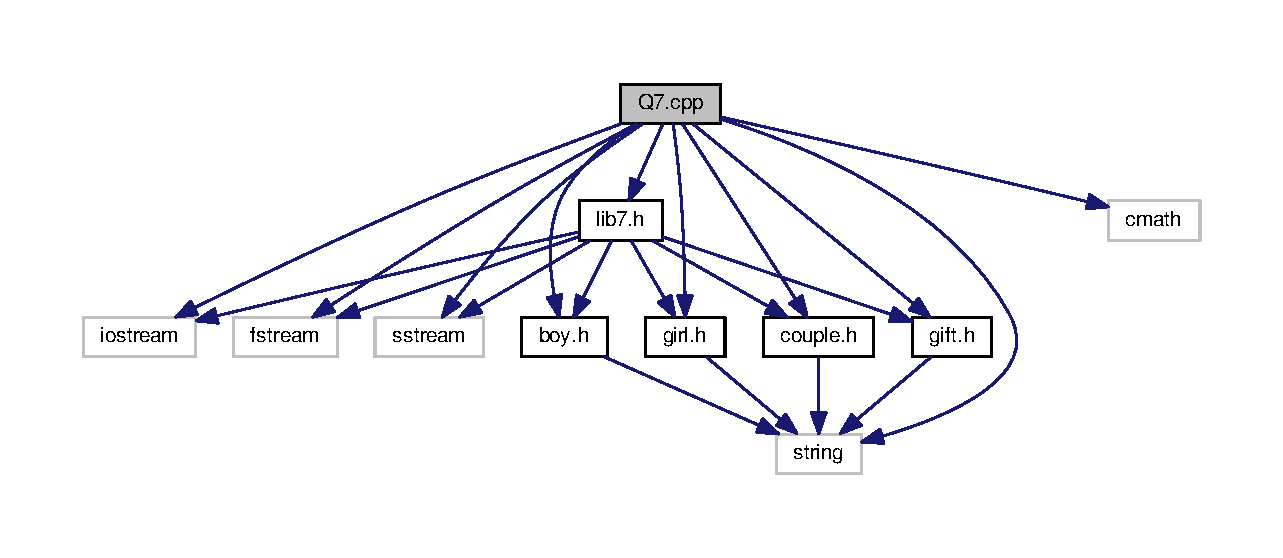
\includegraphics[width=350pt]{Q7_8cpp__incl}
\end{center}
\end{figure}
\subsection*{Macros}
\begin{DoxyCompactItemize}
\item 
\#define \hyperlink{Q7_8cpp_a22995efd1bf00d607d61f25430f44db2}{C\+H\+O\+I\+CE}~2
\end{DoxyCompactItemize}
\subsection*{Functions}
\begin{DoxyCompactItemize}
\item 
void \hyperlink{Q7_8cpp_ac5c65f5b5ec33f7b8ab8012de336fdb7}{swapC} (\hyperlink{classcouple}{couple} \&a, \hyperlink{classcouple}{couple} \&b)
\item 
int \hyperlink{Q7_8cpp_ae66f6b31b5ad750f1fe042a706a4e3d4}{main} ()
\end{DoxyCompactItemize}


\subsection{Macro Definition Documentation}
\index{Q7.\+cpp@{Q7.\+cpp}!C\+H\+O\+I\+CE@{C\+H\+O\+I\+CE}}
\index{C\+H\+O\+I\+CE@{C\+H\+O\+I\+CE}!Q7.\+cpp@{Q7.\+cpp}}
\subsubsection[{\texorpdfstring{C\+H\+O\+I\+CE}{CHOICE}}]{\setlength{\rightskip}{0pt plus 5cm}\#define C\+H\+O\+I\+CE~2}\hypertarget{Q7_8cpp_a22995efd1bf00d607d61f25430f44db2}{}\label{Q7_8cpp_a22995efd1bf00d607d61f25430f44db2}


\subsection{Function Documentation}
\index{Q7.\+cpp@{Q7.\+cpp}!main@{main}}
\index{main@{main}!Q7.\+cpp@{Q7.\+cpp}}
\subsubsection[{\texorpdfstring{main()}{main()}}]{\setlength{\rightskip}{0pt plus 5cm}int main (
\begin{DoxyParamCaption}
{}
\end{DoxyParamCaption}
)}\hypertarget{Q7_8cpp_ae66f6b31b5ad750f1fe042a706a4e3d4}{}\label{Q7_8cpp_ae66f6b31b5ad750f1fe042a706a4e3d4}
$<$ Read boys data

$<$ Read the gifts

$<$ Create Hashtable

$<$ Copying list of boys 
\begin{DoxyCode}
24 \{
25     ifstream boyPtr(\textcolor{stringliteral}{"boyrec.txt"}, ios::in);
26     ifstream girlPtr(\textcolor{stringliteral}{"girlrec.txt"}, ios::in);
27     ofstream opPtr(\textcolor{stringliteral}{"output.txt"}, ios::out);
28     ifstream giftPtr(\textcolor{stringliteral}{"gifts.txt"}, ios::in);
29     ofstream giftout(\textcolor{stringliteral}{"giftslog.txt"}, ios::out);
30     ofstream logfile(\textcolor{stringliteral}{"logfile7.txt"}, ios::out);
31 
32     \textcolor{keywordtype}{int} \hyperlink{lib7_8h_aeee5e31bf47987f4c471a1649ec9e43f}{noBoys} = 9,\hyperlink{lib7_8h_afbf77341ebcfec44fd5ed146e13668bf}{noGirls} = 6;
33     \hyperlink{classBoy}{Boy} boy[\hyperlink{lib7_8h_aeee5e31bf47987f4c471a1649ec9e43f}{noBoys}];
34     \hyperlink{classGirl}{Girl} girl[\hyperlink{lib7_8h_afbf77341ebcfec44fd5ed146e13668bf}{noGirls}];
35     \hyperlink{classcouple}{couple} \hyperlink{classcouple}{couple}[\hyperlink{lib7_8h_afbf77341ebcfec44fd5ed146e13668bf}{noGirls}];
36     \hyperlink{classLibrary}{Library} ob;
37     \hyperlink{classGift}{Gift} gift[4*\hyperlink{lib7_8h_afbf77341ebcfec44fd5ed146e13668bf}{noGirls}];
38     \textcolor{keywordtype}{int} maint, budget,intelli,attr,i;
39     \textcolor{keywordtype}{string} name,girlName,boyName,type;
40     
42     \textcolor{keywordflow}{for}( i = 0; i < \hyperlink{lib7_8h_aeee5e31bf47987f4c471a1649ec9e43f}{noBoys}; i++) \{
43         boyPtr >> name >> type >>attr >> intelli >> budget ;
44         boy[i].\hyperlink{classBoy_aa6d16a472a01b4e7da0817fe94d9a2bd}{init}(name,type,attr,intelli,budget);
45     \}
46 
48     \textcolor{keywordflow}{for}( i = 0; i < \hyperlink{lib7_8h_afbf77341ebcfec44fd5ed146e13668bf}{noGirls}; i++) \{
49         girlPtr >> name >> type >> attr >> intelli >> maint ;
50         girl[i].\hyperlink{classGirl_aba849734c908a23bde2e5bd9c335c450}{init}(name,type,attr,intelli,budget);
51     \}
52 
54     \textcolor{keywordtype}{int} j = 0,k = 0,ind = 0;
55     \textcolor{keywordflow}{for}( i = 0; i < \hyperlink{lib7_8h_afbf77341ebcfec44fd5ed146e13668bf}{noGirls}; i++) \{
56         maint = girl[i].\hyperlink{classGirl_ac23543169a5e339a3c93fbd8aeb977ca}{getMaint}();
57         girlName = girl[i].\hyperlink{classGirl_a27a705fb94b92dfd6929d0bf4bcaf5e1}{getName}();
58         \textcolor{keywordflow}{for}( j = k; j < \hyperlink{lib7_8h_aeee5e31bf47987f4c471a1649ec9e43f}{noBoys}; j++) \{
59             budget = boy[j].\hyperlink{classBoy_a05c48b12091ebcad44ba86ba88514ac5}{getBudget}();
60             boyName = boy[j].\hyperlink{classBoy_acf59fd0074a6ea3413751a95b2970303}{getName}();
61             \textcolor{keywordflow}{if}(maint < budget && !(girl[i].getStatus() ) && !(boy[j].getStatus() ) ) \{
62                     opPtr << girlName << \textcolor{stringliteral}{"        "} << boyName << endl;
63                     couple[i].\hyperlink{classcouple_a3ee36a530603865ff58470bae84da220}{init}(boyName,boy[j].getType(), girlName,boy[j].getBudget(),girl[i].
      getMaint(),boy[j].getAttr(),girl[i].getAttr(),boy[j].getIntelli(),girl[i].getIntelli());
64                     girl[i].\hyperlink{classGirl_ac4e040efdf40d12044bda1b647e0d2da}{changeStatus}();
65                     boy[j].\hyperlink{classBoy_a2a8cc82d9332c07eb475198e46028d52}{changeStatus}();
66                     k++;
67                     \textcolor{keywordflow}{break};
68             \} \textcolor{keywordflow}{else} \{
69                 j--;
70             \}
71         \}
72     \}
73 
74     \textcolor{keywordtype}{int} val,pr;
75     std:: string ty;
77     \textcolor{keywordflow}{for}(i = 0; i < 14; i++) \{
78         giftPtr >> val >> pr >> ty;
79         gift[i].\hyperlink{classGift_aee7c5672f4d1ee738a7dbeb6f952fe1f}{init}(val,pr,ty);
80     \}
81     
83     ob.\hyperlink{classLibrary_a6c32f4296982c3281d61d12b1add0ede}{couples} = couple;
84 
86     \textcolor{keywordflow}{for}(i = 0; i < \hyperlink{lib7_8h_afbf77341ebcfec44fd5ed146e13668bf}{noGirls}; i++) \{
87         ob.\hyperlink{classLibrary_ac6f3af3c59edb37adb8d0becda498b42}{hashCouples}[i].\hyperlink{classcouple_a3ee36a530603865ff58470bae84da220}{init}(\textcolor{stringliteral}{""},boy[j].getType(), \textcolor{stringliteral}{""},boy[j].getBudget(),girl[i].getMaint()
      ,boy[j].getAttr(),girl[i].getAttr(),boy[j].getIntelli(),girl[i].getIntelli())
88     \}
89     \textcolor{keywordflow}{for}(i = 0; i < \hyperlink{lib7_8h_afbf77341ebcfec44fd5ed146e13668bf}{noGirls}; i++) \{
90         \textcolor{keywordtype}{int} ind = (couple[i].\hyperlink{classcouple_afe07f86e775d20508e6cd139488af366}{getBoyname}()[0] + 7)%noGirls;
91         \textcolor{keywordflow}{while}( couple[ind].getBoyname() != \textcolor{stringliteral}{""}) ind = (ind + 1) % \hyperlink{lib7_8h_afbf77341ebcfec44fd5ed146e13668bf}{noGirls};
92         ob.\hyperlink{classLibrary_ac6f3af3c59edb37adb8d0becda498b42}{hashCouples}[ind] = couple[i];
93     \}
94 
96     \textcolor{keywordflow}{for}(i = 0; i < \hyperlink{lib7_8h_afbf77341ebcfec44fd5ed146e13668bf}{noGirls}; i++) \{
97         \textcolor{keywordflow}{for}( j = i+1; j< \hyperlink{lib7_8h_afbf77341ebcfec44fd5ed146e13668bf}{noGirls}; j++) \{
98             \textcolor{keywordflow}{if}( couple[i].getBoyname()[0] > couple[j].\hyperlink{classcouple_afe07f86e775d20508e6cd139488af366}{getBoyname}()[0]) \{
99                 \hyperlink{Q7_8cpp_ac5c65f5b5ec33f7b8ab8012de336fdb7}{swapC}(couple[i],couple[j]);
100             \}
101         \}
102     \}
103 
104     ob.sortedcouples = couple;
105 
106     logFile<<\textcolor{stringliteral}{"\(\backslash\)n-----------List of Boys----------\(\backslash\)n\(\backslash\)n"};
108     \textcolor{keywordflow}{for}(i = 0; i< \hyperlink{lib7_8h_aeee5e31bf47987f4c471a1649ec9e43f}{noBoys}; i++) \{
109         ob.\hyperlink{classLibrary_a0da9d216b9e07af39f5f0f3241a0a45c}{boysList}[i] = boy[i];
110         logFile<<\textcolor{stringliteral}{"b"}<<ob.\hyperlink{classLibrary_a0da9d216b9e07af39f5f0f3241a0a45c}{boysList}[i].getBoyname()<<\textcolor{stringliteral}{" "};
111     \}   
112 
114     \textcolor{keywordtype}{int} choice = \hyperlink{Q7_8cpp_a22995efd1bf00d607d61f25430f44db2}{CHOICE};
115     \textcolor{keywordflow}{switch}(choice) \{
116         \textcolor{keywordflow}{case} 1: 
117             ob.\hyperlink{classLibrary_af9853cceb7af37b77091c3330b532b2f}{searchArr}();
118             \textcolor{keywordflow}{break};
119         \textcolor{keywordflow}{case} 2:     \textcolor{comment}{//for binary search}
120             ob.\hyperlink{classLibrary_a835ea2c0b31c569aac4a406843c55254}{searchSortedArr}();
121             \textcolor{keywordflow}{break};
122         \textcolor{keywordflow}{case} 3:     \textcolor{comment}{//for using hashtable}
123             cout<<choice<<endl;
124             ob.\hyperlink{classLibrary_ad14b4301aa6279c13408ff948ca4fd6a}{searchHash}();
125             \textcolor{keywordflow}{break};
126     \}
127 
128 \}
\end{DoxyCode}
\index{Q7.\+cpp@{Q7.\+cpp}!swapC@{swapC}}
\index{swapC@{swapC}!Q7.\+cpp@{Q7.\+cpp}}
\subsubsection[{\texorpdfstring{swap\+C(couple \&a, couple \&b)}{swapC(couple &a, couple &b)}}]{\setlength{\rightskip}{0pt plus 5cm}void swapC (
\begin{DoxyParamCaption}
\item[{{\bf couple} \&}]{a, }
\item[{{\bf couple} \&}]{b}
\end{DoxyParamCaption}
)}\hypertarget{Q7_8cpp_ac5c65f5b5ec33f7b8ab8012de336fdb7}{}\label{Q7_8cpp_ac5c65f5b5ec33f7b8ab8012de336fdb7}

\begin{DoxyCode}
17 \{
18     \hyperlink{classcouple}{couple} temp = a;
19     a = b;
20     b = temp;
21 \}
\end{DoxyCode}

\hypertarget{Q8_8cpp}{}\section{Q8.\+cpp File Reference}
\label{Q8_8cpp}\index{Q8.\+cpp@{Q8.\+cpp}}
{\ttfamily \#include \char`\"{}lib8.\+h\char`\"{}}\\*
Include dependency graph for Q8.\+cpp\+:
\nopagebreak
\begin{figure}[H]
\begin{center}
\leavevmode
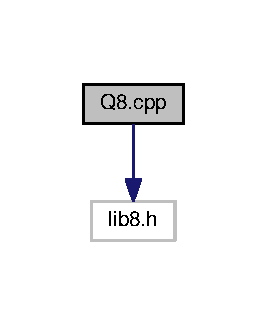
\includegraphics[width=128pt]{Q8_8cpp__incl}
\end{center}
\end{figure}

\hypertarget{Q9_8cpp}{}\section{Q9.\+cpp File Reference}
\label{Q9_8cpp}\index{Q9.\+cpp@{Q9.\+cpp}}
{\ttfamily \#include $<$iostream$>$}\\*
{\ttfamily \#include $<$fstream$>$}\\*
{\ttfamily \#include $<$sstream$>$}\\*
{\ttfamily \#include $<$cmath$>$}\\*
{\ttfamily \#include \char`\"{}boy.\+h\char`\"{}}\\*
{\ttfamily \#include \char`\"{}girl.\+h\char`\"{}}\\*
{\ttfamily \#include \char`\"{}couple.\+h\char`\"{}}\\*
{\ttfamily \#include \char`\"{}gift.\+h\char`\"{}}\\*
Include dependency graph for Q9.\+cpp\+:
\nopagebreak
\begin{figure}[H]
\begin{center}
\leavevmode
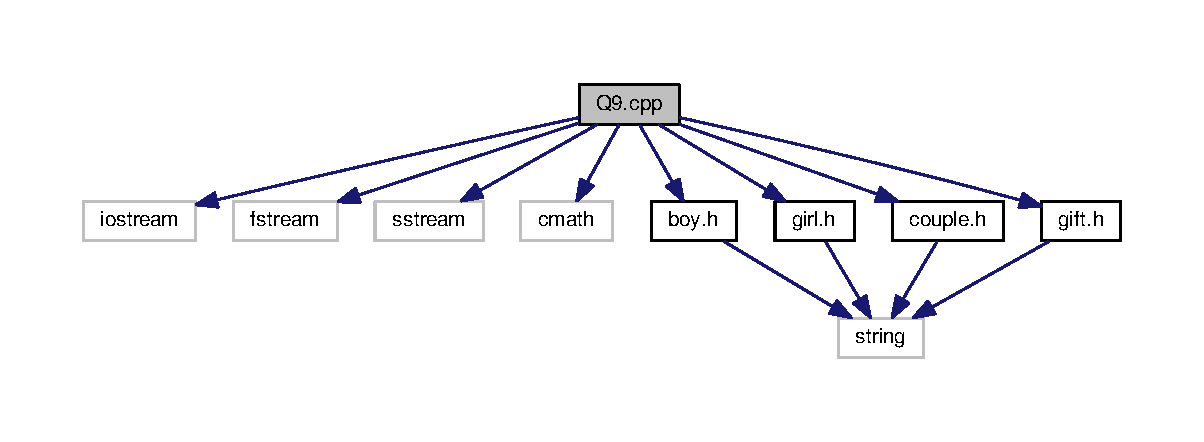
\includegraphics[width=350pt]{Q9_8cpp__incl}
\end{center}
\end{figure}
\subsection*{Macros}
\begin{DoxyCompactItemize}
\item 
\#define \hyperlink{Q9_8cpp_a111da81ae5883147168bbb8366377b10}{B}~9
\item 
\#define \hyperlink{Q9_8cpp_aed9ea78689ecce0b7264c02c7f8a9a54}{G}~5
\item 
\#define \hyperlink{Q9_8cpp_ac4cf4b2ab929bd23951a8676eeac086b}{C}~5
\item 
\#define \hyperlink{Q9_8cpp_a5e0c07e523d4e77a2cafca06feb836f6}{Gf}~15
\item 
\#define \hyperlink{Q9_8cpp_a97d832ae23af4f215e801e37e4f94254}{K}~2
\end{DoxyCompactItemize}
\subsection*{Functions}
\begin{DoxyCompactItemize}
\item 
void \hyperlink{Q9_8cpp_ac70f752855ee1cf9ceaa2d749bbad17d}{swap} (\hyperlink{classGift}{Gift} \&a, \hyperlink{classGift}{Gift} \&b)
\item 
void \hyperlink{Q9_8cpp_a9ed5e5ebda90f206f83cd424ebebe79d}{swapC} (Couple \&a, Couple \&b)
\item 
{\footnotesize template$<$class T $>$ }\\void \hyperlink{Q9_8cpp_afb2bbadfe7cfd2620d67ca6d0ccb2411}{sorting\+Datastructure} (\hyperlink{Q6_8cpp_a0acb682b8260ab1c60b918599864e2e5}{T} $\ast$arr, int n, int k, string s)
\item 
int \hyperlink{Q9_8cpp_ae66f6b31b5ad750f1fe042a706a4e3d4}{main} ()
\end{DoxyCompactItemize}


\subsection{Macro Definition Documentation}
\index{Q9.\+cpp@{Q9.\+cpp}!B@{B}}
\index{B@{B}!Q9.\+cpp@{Q9.\+cpp}}
\subsubsection[{\texorpdfstring{B}{B}}]{\setlength{\rightskip}{0pt plus 5cm}\#define B~9}\hypertarget{Q9_8cpp_a111da81ae5883147168bbb8366377b10}{}\label{Q9_8cpp_a111da81ae5883147168bbb8366377b10}
\index{Q9.\+cpp@{Q9.\+cpp}!C@{C}}
\index{C@{C}!Q9.\+cpp@{Q9.\+cpp}}
\subsubsection[{\texorpdfstring{C}{C}}]{\setlength{\rightskip}{0pt plus 5cm}\#define C~5}\hypertarget{Q9_8cpp_ac4cf4b2ab929bd23951a8676eeac086b}{}\label{Q9_8cpp_ac4cf4b2ab929bd23951a8676eeac086b}
\index{Q9.\+cpp@{Q9.\+cpp}!G@{G}}
\index{G@{G}!Q9.\+cpp@{Q9.\+cpp}}
\subsubsection[{\texorpdfstring{G}{G}}]{\setlength{\rightskip}{0pt plus 5cm}\#define G~5}\hypertarget{Q9_8cpp_aed9ea78689ecce0b7264c02c7f8a9a54}{}\label{Q9_8cpp_aed9ea78689ecce0b7264c02c7f8a9a54}
\index{Q9.\+cpp@{Q9.\+cpp}!Gf@{Gf}}
\index{Gf@{Gf}!Q9.\+cpp@{Q9.\+cpp}}
\subsubsection[{\texorpdfstring{Gf}{Gf}}]{\setlength{\rightskip}{0pt plus 5cm}\#define Gf~15}\hypertarget{Q9_8cpp_a5e0c07e523d4e77a2cafca06feb836f6}{}\label{Q9_8cpp_a5e0c07e523d4e77a2cafca06feb836f6}
\index{Q9.\+cpp@{Q9.\+cpp}!K@{K}}
\index{K@{K}!Q9.\+cpp@{Q9.\+cpp}}
\subsubsection[{\texorpdfstring{K}{K}}]{\setlength{\rightskip}{0pt plus 5cm}\#define K~2}\hypertarget{Q9_8cpp_a97d832ae23af4f215e801e37e4f94254}{}\label{Q9_8cpp_a97d832ae23af4f215e801e37e4f94254}


\subsection{Function Documentation}
\index{Q9.\+cpp@{Q9.\+cpp}!main@{main}}
\index{main@{main}!Q9.\+cpp@{Q9.\+cpp}}
\subsubsection[{\texorpdfstring{main()}{main()}}]{\setlength{\rightskip}{0pt plus 5cm}int main (
\begin{DoxyParamCaption}
{}
\end{DoxyParamCaption}
)}\hypertarget{Q9_8cpp_ae66f6b31b5ad750f1fe042a706a4e3d4}{}\label{Q9_8cpp_ae66f6b31b5ad750f1fe042a706a4e3d4}
$<$ Read boys data

$<$ Read the gifts

$<$ Sort couples according to their happiness

$<$ Print sorted couple in a file 
\begin{DoxyCode}
51 \{
52     ifstream boyPtr(\textcolor{stringliteral}{"boyrec.txt"}, ios::in);
53     ifstream girlPtr(\textcolor{stringliteral}{"girlrec.txt"}, ios::in);
54     ofstream opPtr(\textcolor{stringliteral}{"output.txt"}, ios::out);
55     ifstream giftPtr(\textcolor{stringliteral}{"gifts.txt"}, ios::in);
56     ofstream giftout(\textcolor{stringliteral}{"giftslog.txt"}, ios::out);
57 
58     \textcolor{keywordtype}{int} \hyperlink{lib7_8h_aeee5e31bf47987f4c471a1649ec9e43f}{noBoys} = 9,\hyperlink{lib7_8h_afbf77341ebcfec44fd5ed146e13668bf}{noGirls} = 6;
59     \hyperlink{classBoy}{Boy} boy[\hyperlink{lib7_8h_aeee5e31bf47987f4c471a1649ec9e43f}{noBoys}];
60     \hyperlink{classGirl}{Girl} girl[\hyperlink{lib7_8h_afbf77341ebcfec44fd5ed146e13668bf}{noGirls}];
61     \hyperlink{classcouple}{couple} \hyperlink{classcouple}{couple}[\hyperlink{lib7_8h_afbf77341ebcfec44fd5ed146e13668bf}{noGirls}];
62     \hyperlink{classGift}{Gift} gift[4*\hyperlink{lib7_8h_afbf77341ebcfec44fd5ed146e13668bf}{noGirls}];
63     \textcolor{keywordtype}{int} maint, budget,intelli,attr,i;
64     \textcolor{keywordtype}{string} name,girlName,boyName,type;
65     
67     \textcolor{keywordflow}{for}( i = 0; i < \hyperlink{lib7_8h_aeee5e31bf47987f4c471a1649ec9e43f}{noBoys}; i++) \{
68         boyPtr >> name >> type >>attr >> intelli >> budget ;
69         boy[i].\hyperlink{classBoy_aa6d16a472a01b4e7da0817fe94d9a2bd}{init}(name,type,attr,intelli,budget);
70     \}
71 
73     \textcolor{keywordflow}{for}( i = 0; i < \hyperlink{lib7_8h_afbf77341ebcfec44fd5ed146e13668bf}{noGirls}; i++) \{
74         girlPtr >> name >> type >> attr >> intelli >> maint ;
75         girl[i].\hyperlink{classGirl_aba849734c908a23bde2e5bd9c335c450}{init}(name,type,attr,intelli,budget);
76     \}
77 
79     \textcolor{keywordtype}{int} j = 0,k = 0,ind = 0;
80     \textcolor{keywordflow}{for}( i = 0; i < \hyperlink{lib7_8h_afbf77341ebcfec44fd5ed146e13668bf}{noGirls}; i++) \{
81         maint = girl[i].\hyperlink{classGirl_ac23543169a5e339a3c93fbd8aeb977ca}{getMaint}();
82         girlName = girl[i].\hyperlink{classGirl_a27a705fb94b92dfd6929d0bf4bcaf5e1}{getName}();
83         \textcolor{keywordflow}{for}( j = k; j < \hyperlink{lib7_8h_aeee5e31bf47987f4c471a1649ec9e43f}{noBoys}; j++) \{
84             budget = boy[j].\hyperlink{classBoy_a05c48b12091ebcad44ba86ba88514ac5}{getBudget}();
85             boyName = boy[j].\hyperlink{classBoy_acf59fd0074a6ea3413751a95b2970303}{getName}();
86             \textcolor{keywordflow}{if}(maint < budget && !(girl[i].getStatus() ) && !(boy[j].getStatus() ) ) \{
87                     opPtr << girlName << \textcolor{stringliteral}{"        "} << boyName << endl;
88                     couple[i].\hyperlink{classcouple_a3ee36a530603865ff58470bae84da220}{init}(boyName,boy[j].getType(), girlName,boy[j].getBudget(),girl[i].
      getMaint(),boy[j].getAttr(),girl[i].getAttr(),boy[j].getIntelli(),girl[i].getIntelli());
89                     girl[i].\hyperlink{classGirl_ac4e040efdf40d12044bda1b647e0d2da}{changeStatus}();
90                     boy[j].\hyperlink{classBoy_a2a8cc82d9332c07eb475198e46028d52}{changeStatus}();
91                     k++;
92                     \textcolor{keywordflow}{break};
93             \} \textcolor{keywordflow}{else} \{
94                 j--;
95             \}
96         \}
97     \}
98 
99     \textcolor{keywordtype}{int} val,pr;
100     std:: string ty;
102     \textcolor{keywordflow}{for}(i = 0; i < 14; i++) \{
103         giftPtr >> val >> pr >> ty;
104         gift[i].\hyperlink{classGift_aee7c5672f4d1ee738a7dbeb6f952fe1f}{init}(val,pr,ty);
105     \}
107     \textcolor{keywordtype}{int} currbud;
108     j = 0;
109     \textcolor{keywordflow}{for}(i = 0; i < \hyperlink{lib7_8h_afbf77341ebcfec44fd5ed146e13668bf}{noGirls}; i++) \{
110         currbud = couple[i].\hyperlink{classcouple_af4b090a72111d7ba566747e4e305a6ec}{getCurrBudget}() ;
111         \textcolor{keywordflow}{while}(currbud > gift[j].getPrice() && j < 14) \{
112             pr = gift[j].\hyperlink{classGift_aa114ca9629b5f02e4df6731d33c69373}{getPrice}();
113             giftout << couple[i].\hyperlink{classcouple_afe07f86e775d20508e6cd139488af366}{getBoyname}() << \textcolor{stringliteral}{"  "} << couple[i].
      \hyperlink{classcouple_a7897320b780dbeaa85380c71803de9c2}{getGirlname}() << \textcolor{stringliteral}{"  "} <<  pr << endl;
114             couple[i].\hyperlink{classcouple_afa9889ca750dd53ffd06daf78cbee326}{changeCurrBudget}(pr);
115             j++;
116             currbud = couple[i].\hyperlink{classcouple_af4b090a72111d7ba566747e4e305a6ec}{getCurrBudget}() ;
117         \}
118     \}
119     \textcolor{comment}{/*}
120 \textcolor{comment}{    * Calculate Happiness of Girls
}
121 \textcolor{comment}{    */}
122     \textcolor{keywordtype}{int} bh,gh,cost;
123     \textcolor{keywordflow}{for}( i = 0; i< \hyperlink{lib7_8h_afbf77341ebcfec44fd5ed146e13668bf}{noGirls}; i++) \{
124         type = girl[i].\hyperlink{classGirl_a2b5bbd35287b7aa074f39702b564bc97}{getType}();
125         cost = couple[i].\hyperlink{classcouple_a5f31ac8019f5db29694dc36cdba958b8}{getCost}();
126         \textcolor{keywordflow}{if}(type == \textcolor{stringliteral}{"Choosy"}) \{
127             gh = log10(cost / girl[i].getMaint());
128         \} \textcolor{keywordflow}{else} \textcolor{keywordflow}{if}(type == \textcolor{stringliteral}{"Normal"}) \{
129             gh = cost / girl[i].\hyperlink{classGirl_ac23543169a5e339a3c93fbd8aeb977ca}{getMaint}();
130         \} \textcolor{keywordflow}{else} \textcolor{keywordflow}{if}(type == \textcolor{stringliteral}{"Desperate"}) \{
131             gh = exp(cost / girl[i].getMaint());
132         \}
133         couple[i].\hyperlink{classcouple_a526f48a752f261212d111a630f5730f4}{setGirlHappiness}(gh);
134     \}
135  
137     \textcolor{keywordflow}{for}(i = 0; i < \hyperlink{lib7_8h_afbf77341ebcfec44fd5ed146e13668bf}{noGirls}; i++) \{
138         type = couple[i].\hyperlink{classcouple_a687986a266cc984fa5d2114c888f52cf}{getBoyType}();
139         cost = couple[i].\hyperlink{classcouple_a5f31ac8019f5db29694dc36cdba958b8}{getCost}();
140         \textcolor{keywordflow}{if}(type == \textcolor{stringliteral}{"Miser"}) \{
141             bh = couple[i].\hyperlink{classcouple_a92496b42f9d1392013c4d7456318ad70}{getBudget}() - cost;
142         \} \textcolor{keywordflow}{else} \textcolor{keywordflow}{if}(type == \textcolor{stringliteral}{"Generous"}) \{
143             bh = couple[i].\hyperlink{classcouple_ada2f9b79cede186a0e9bcd6b48bec804}{getGirlHappiness}();
144         \} \textcolor{keywordflow}{else} \{
145             bh = girl[i].\hyperlink{classGirl_afe73c4c4f180aa8f5e0bc4f87455ec0b}{getIntelligence}();
146         \}
147         couple[i].\hyperlink{classcouple_a50a890cb7ffd3a44f0201b8e0d84f744}{setBoyHappiness}(bh);
148         couple[i].\hyperlink{classcouple_aaaadc39a9f265907581925ef579c7214}{setHappiness}();
149     \}
150 
151     \textcolor{keywordtype}{int} h1,h2;
152 
153     k = 3;
155     \textcolor{keywordflow}{for}(i = 0; i < \hyperlink{lib7_8h_afbf77341ebcfec44fd5ed146e13668bf}{noGirls}; i++) \{
156         h1 = couple[i].\hyperlink{classcouple_a31d0a1c8acff06a64ebc2e2f6d9a68b1}{getHappiness}();
157         \textcolor{keywordflow}{for}(j = i+1; j < \hyperlink{lib7_8h_afbf77341ebcfec44fd5ed146e13668bf}{noGirls}; j++) \{
158             h2 = couple[j].\hyperlink{classcouple_a31d0a1c8acff06a64ebc2e2f6d9a68b1}{getHappiness}();
159             \textcolor{keywordflow}{if}(h1 > h2) \{
160                 \hyperlink{Q2_8cpp_a5a408068bacb1c7add72673eb9d96bbc}{swapCouple}(couple[i], couple[j]);
161             \}
162         \}
163     \}
164 
165     ofstream happiness(\textcolor{stringliteral}{"sortedHappiness.txt"}, ios::out);
166     ofstream compatibility(\textcolor{stringliteral}{"sortedComaptibility.txt"}, ios::out);
167 
169     \textcolor{keywordflow}{for}(i = 0; i< k; i++) \{
170         happiness << couple[i].\hyperlink{classcouple_afe07f86e775d20508e6cd139488af366}{getBoyname}() << \textcolor{stringliteral}{"  "} << couple[i].
      \hyperlink{classcouple_a7897320b780dbeaa85380c71803de9c2}{getGirlname}() <<  \textcolor{stringliteral}{"   "} << couple[i].\hyperlink{classcouple_a31d0a1c8acff06a64ebc2e2f6d9a68b1}{getHappiness}() << endl;
171     \}
172 
174     \textcolor{keywordflow}{for}( i = 0; i < \hyperlink{lib7_8h_afbf77341ebcfec44fd5ed146e13668bf}{noGirls}; i++) \{
175         couple[i].\hyperlink{classcouple_a91bc77488fe8b5d30643b9ff0a56d359}{setCompatibility}();
176     \}
177 
179     \textcolor{keywordflow}{for}(i = 0; i < \hyperlink{lib7_8h_afbf77341ebcfec44fd5ed146e13668bf}{noGirls}; i++) \{
180         h1 = couple[i].\hyperlink{classcouple_a43d2852ce692307280ba9ab2366c16eb}{getCompatibility}();
181         \textcolor{keywordflow}{for}(j = i+1; j < \hyperlink{lib7_8h_afbf77341ebcfec44fd5ed146e13668bf}{noGirls}; j++) \{
182             h2 = couple[j].\hyperlink{classcouple_a43d2852ce692307280ba9ab2366c16eb}{getCompatibility}();
183             \textcolor{keywordflow}{if}(h1 > h2) \{
184                 \hyperlink{Q9_8cpp_a9ed5e5ebda90f206f83cd424ebebe79d}{swapC}(couple[i],couple[j]);
185             \}
186         \}
187     \}
188 
190     \textcolor{keywordflow}{for}(i = 0; i< k; i++) \{
191         compatibility << couple[i].\hyperlink{classcouple_afe07f86e775d20508e6cd139488af366}{getBoyname}() << \textcolor{stringliteral}{"  "} << couple[i].
      \hyperlink{classcouple_a7897320b780dbeaa85380c71803de9c2}{getGirlname}() << endl;
192     \}
193 
194 \}
\end{DoxyCode}
\index{Q9.\+cpp@{Q9.\+cpp}!sorting\+Datastructure@{sorting\+Datastructure}}
\index{sorting\+Datastructure@{sorting\+Datastructure}!Q9.\+cpp@{Q9.\+cpp}}
\subsubsection[{\texorpdfstring{sorting\+Datastructure(\+T $\ast$arr, int n, int k, string s)}{sortingDatastructure(T *arr, int n, int k, string s)}}]{\setlength{\rightskip}{0pt plus 5cm}template$<$class T $>$ void sorting\+Datastructure (
\begin{DoxyParamCaption}
\item[{{\bf T} $\ast$}]{arr, }
\item[{int}]{n, }
\item[{int}]{k, }
\item[{string}]{s}
\end{DoxyParamCaption}
)}\hypertarget{Q9_8cpp_afb2bbadfe7cfd2620d67ca6d0ccb2411}{}\label{Q9_8cpp_afb2bbadfe7cfd2620d67ca6d0ccb2411}

\begin{DoxyCode}
37 \{
38     \textcolor{keywordflow}{for}(\textcolor{keywordtype}{int} i = 0  ; i< n-1; i++) \{
39         \textcolor{keywordflow}{for}(\textcolor{keywordtype}{int} j = i+1; j < n; j++) \{
40              \textcolor{keywordflow}{if}(s == \textcolor{stringliteral}{"attractiveness"}) \{
41                 \textcolor{keywordflow}{if}(arr[j].getAttractiveness() < arr[i].getAttractiveness()) \{
42                     \hyperlink{Q9_8cpp_ac70f752855ee1cf9ceaa2d749bbad17d}{swap}(arr[j],arr[i]);
43                 \}
44             \}
45         \}
46     \}
47 \}
\end{DoxyCode}
\index{Q9.\+cpp@{Q9.\+cpp}!swap@{swap}}
\index{swap@{swap}!Q9.\+cpp@{Q9.\+cpp}}
\subsubsection[{\texorpdfstring{swap(\+Gift \&a, Gift \&b)}{swap(Gift &a, Gift &b)}}]{\setlength{\rightskip}{0pt plus 5cm}void swap (
\begin{DoxyParamCaption}
\item[{{\bf Gift} \&}]{a, }
\item[{{\bf Gift} \&}]{b}
\end{DoxyParamCaption}
)}\hypertarget{Q9_8cpp_ac70f752855ee1cf9ceaa2d749bbad17d}{}\label{Q9_8cpp_ac70f752855ee1cf9ceaa2d749bbad17d}

\begin{DoxyCode}
21 \{
22     \hyperlink{classGift}{Gift} temp = a;
23     a = b;
24     b = temp;
25 \}
\end{DoxyCode}
\index{Q9.\+cpp@{Q9.\+cpp}!swapC@{swapC}}
\index{swapC@{swapC}!Q9.\+cpp@{Q9.\+cpp}}
\subsubsection[{\texorpdfstring{swap\+C(\+Couple \&a, Couple \&b)}{swapC(Couple &a, Couple &b)}}]{\setlength{\rightskip}{0pt plus 5cm}void swapC (
\begin{DoxyParamCaption}
\item[{Couple \&}]{a, }
\item[{Couple \&}]{b}
\end{DoxyParamCaption}
)}\hypertarget{Q9_8cpp_a9ed5e5ebda90f206f83cd424ebebe79d}{}\label{Q9_8cpp_a9ed5e5ebda90f206f83cd424ebebe79d}

\begin{DoxyCode}
28 \{
29     Couple temp = a;
30     a = b;
31     b = temp;
32 \}
\end{DoxyCode}

\hypertarget{README_8md}{}\section{R\+E\+A\+D\+M\+E.\+md File Reference}
\label{README_8md}\index{R\+E\+A\+D\+M\+E.\+md@{R\+E\+A\+D\+M\+E.\+md}}

\hypertarget{sortedComaptibility_8txt}{}\section{sorted\+Comaptibility.\+txt File Reference}
\label{sortedComaptibility_8txt}\index{sorted\+Comaptibility.\+txt@{sorted\+Comaptibility.\+txt}}

\hypertarget{sortedCompatibility_8txt}{}\section{sorted\+Compatibility.\+txt File Reference}
\label{sortedCompatibility_8txt}\index{sorted\+Compatibility.\+txt@{sorted\+Compatibility.\+txt}}

\hypertarget{sortedHappiness_8txt}{}\section{sorted\+Happiness.\+txt File Reference}
\label{sortedHappiness_8txt}\index{sorted\+Happiness.\+txt@{sorted\+Happiness.\+txt}}

%--- End generated contents ---

% Index
\backmatter
\newpage
\phantomsection
\clearemptydoublepage
\addcontentsline{toc}{chapter}{Index}
\printindex

\end{document}
